\chapter{Модификация двойного каскада для обогащения регенерированного урана в условиях многократного рецикла}\label{ch:ch3}

\section{Разработка каскадной схемы для обогащения регенерированного урана с одновременным выполнением условия на отношение используемого регенерата по отношению к производимому продукту, а также ограничений на концентрации четных изотопов}
\subsection{Описание предлагаемой схемы}\label{triple_descr}

Основной проблемой, подлежащей решению в настоящей работе, является поиск варианта каскадной схемы, позволяющей одновременно выполнить условия по четным изотопам и задействовать в обогащении весь поступивший регенерат при различных внешних условиях и различных исходных составах регенерата.

Невозможность возврата регенерата в производство топлива с использованием многочисленных модификаций каскада для обогащения многократно облученного регенерата, во многом, связана с ростом величин относительных концентраций «легких» изотопов (в первую очередь $^{232}$U) по отношению к $^{235}$U в поступающем в обогащении регенерате. Далее, в процессе обогащения относительные концентрации легких изотопов по отношению к $^{235}$U также возрастают. Это связано с тем, что при обогащении $^{235}$U более легкие изотопы концентрируются вместе с ним. При использовании схем на основе одиночного ординарного каскада единственным способом понизить относительную концентрацию изотопов  $^{232}$U и $^{235}$U является разбавление смеси обогащаемого регенерата материалом, не содержащим $^{232}$U, например на входе в каскад \cite{smirnovKaskadnyeShemyZadachah2012}. Однако, результаты вычислительных экспериментов, проведенных для различных разбавителей показывают, что для составов с высоким исходным содержанием $^{232}$U (выше предельных значений для товарного НОУ) невозможно подобрать разбавитель такой, чтобы удовлетворить одновременно условия полного возврата регенерата в цикл и заданные ограничения на концентрации четных изотопов в товарном продукте (см. Главу \ref{ch:ch2}). 

Решение данной проблемы может быть основано на использовании двойных каскадов, позволяющих частично отделить друг от друга изотопы $^{232}$U и $^{235}$U, что позволяет выполнить ограничения на концентрации четных изотопов в товарном НОУ без разбавления регенерата сырьем, не содержащим $^{232}$U и $^{236}$U. Однако, как показано в Главе 3, простой вариант двойного каскада имеет определенные недостатки, стимулирующие поиск более эффективных способов решения задачи. 

Предлагаемый вариант каскадной схемы состоит из двух подсистем (рис. \ref{p2left}): первая представляет собой двойной каскад (каскады I и II на рис. \ref{p2left}), вторая представляет собой ординарный каскад для обогащения природного урана (каскад III на рис. \ref{p2left}). В первом каскаде подсистемы I обогащают исходный регенерат изотопами $^{232,233,234,235,236}$U. В каскаде II смесь делится на две фракции, так, чтобы в потоке тяжелой фракции ($W_2$) было понижено содержание $^{232,233,234}$U по отношению к питающей второй каскад смеси -- потоку $P_1$. 

\begin{figure}[ht]
    \centerfloat{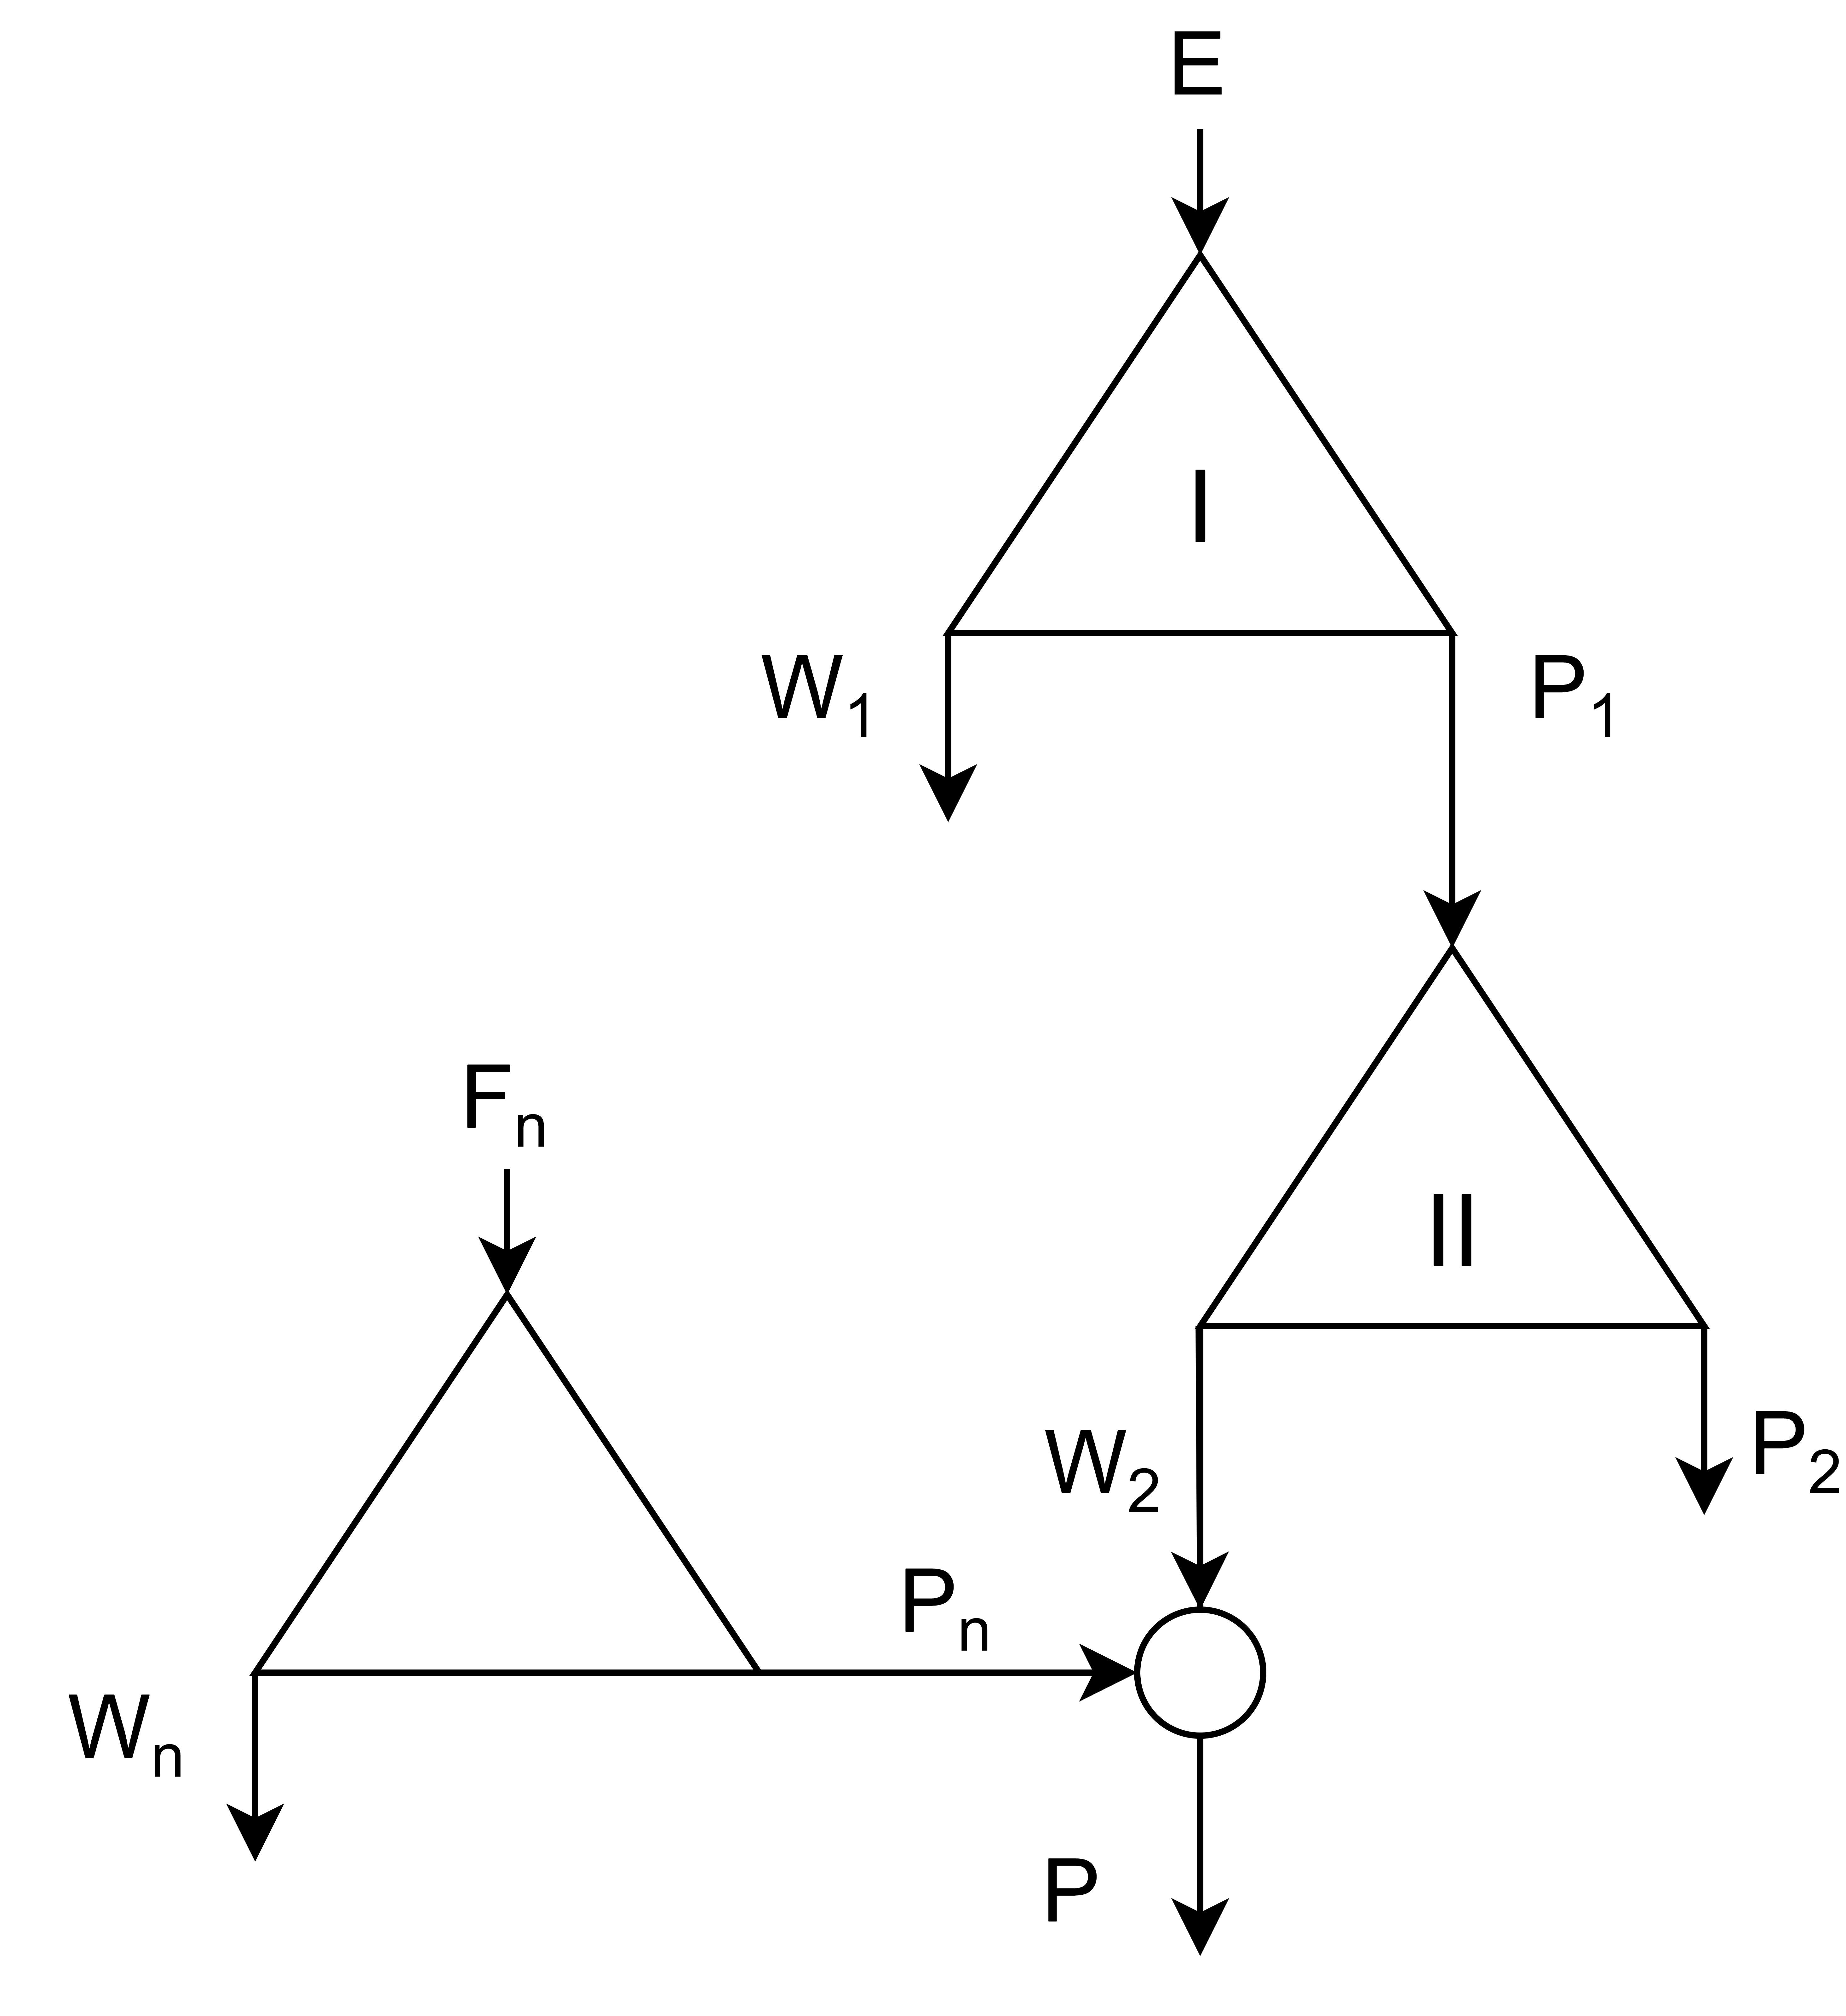
\includegraphics[scale=0.05]{cascades/DoubleModified}}
    \caption{Схема модифицированного двойного каскада для обогащения регенерированного урана. Обозначения: $E$ -- поток регенерированного урана; $P_1$ -- поток отбора первого каскада, выступающий питанием второго каскада; $P_2$ -- поток отбора второго каскада; $W_1$ -- поток отвала первого каскада; $W_2$ -- поток тяжелой фракции (условный «отвал») второго каскада; $P_n$ -- поток НОУ-разбавителя; $P$ -- финальный продукт (товарный низкообогащенный уран (НОУ))}\label{p2left}
\end{figure}

Концентрация $^{235}$U в потоке $P_1$ должна быть больше концентрации $^{235}$U в конечном продукте, ввиду того, что во втором каскаде получаемый продукт будет обедняться по $^{235}$U. Что касается верхней границы концентрации ${C}_{235,{P_1}}$, то она с физической точки зрения может быть ограничена только предельно достижимой концентрацией $^{235}$U в этом потоке, определяемой по известным соотношениям \cite{sulaberidzeOsobennostiObogashcheniyaKomponentov2006}, \cite{minenkoPredelnoeObogashcheniePromezhutochnyh1972}. С другой стороны при задании параметров каскадов подсистемы I необходимо согласовывать значения концентраций ${C}_{235,{P_1}}$ и ${C}_{235,{P_2}}$, поскольку должно выполняться очевидное соотношение ${C}_{235,{P_2}}{>}{C}_{235,{P_1}}$.
% Далее, полученный в первом каскаде обогащенный уран направляется на вход второго каскада, где он разделяется на 2 группы: в первой концентрируются легкие изотопы и $^{235}$U, во второй легкие изотопы обедняются, параллельно с относительно небольшим снижением концентрации $^{235}$U.
Выбор $C_{235,{P_2}}$ может определяться не только физическими соображениями, но и формальными. Учитывая, что поток $P_2$ является одним из внешних, выходящих из схемы рис. \ref{p2left} потоков, то на него могут распространяться, например, требования о непревышение порога обогащения в 20\%. Такое ограничение обусловлено тем, что уран, обогащенный до 20\% и выше, по критериям МАГАТЭ считают материалом прямого использования, т.е. пригодным для создания ядерно-взрывных устройств \cite{brownOriginsSignificanceLimit2016}, \cite{pshakinYadernoeNerasprostranenie2006}. Превышение данного порога может оказаться критичным с формальной с точки зрения нормативных документов, однако данное ограничение не является физическим, что позволяет потенциально рассматривать и значения концентраций  $C_{235,{P_2}}$ выше этой величины. 

Финальным шагом к получению конечного НОУ-продукта является разбавление потока $W_2$ второго каскада сырьем, не содержащим искусственных изотопов урана для выполнения ограничений по $^{232}$U и $^{236}$U.
Для этого используют вторую подсистему (каскад III), предназначенную для наработки разбавителя заданной массы и заданного обогащения по $^{235}$U.
Необходимо учесть то, что при заданных концентрациях $^{235}$U в потоках ${P_1}, {W_1}, {P_2}, {W_2}$ и отношении потоков $E/P$, отношение потоков ${W_2}{/P}$ также будет заданным, что подтверждает приведенное ниже выражение:

\begin{equation}
    \label{dc1}
    \frac{W_{2}}{P}=\frac{P_{1}}{E}\cdot\frac{W_{2}}{P_{1}}\cdot\frac{E}{P}
\end{equation}

, где $E$ -- поток исходного регенерата, а $P$ -- поток конечного продукта НОУ-продукта.

В дополнение к \ref{dc1} запишем очевидное равенство:

\begin{equation}
    \label{dc2}
    \frac{P_{0}}{P} = 1 - \frac{W_{2}}{P}
\end{equation}

Из \ref{dc1} и \ref{dc2} следует, что отношение потоков ${W_2}{/}{P_0}$ также будет заданным. Иными словами, соотношение между потоками $W_2$ и $P_0$ при их смешивании зависит от выбора параметров каскадов подсистемы I. В этом случае единственным параметром, влияющим на концентрацию $^{235}$U в товарном НОУ является концентрация данного изотопа в разбавителе (поток $P_0$ на схеме рис. \ref{p2left}), которая связана с остальными параметрами соотношением, выражающим закон сохранения вещества для узла смешивания потоков $W_2$ и $P_0$: 

\begin{equation}
    \label{dc3}
    C_{235,P_{0}}=C_{235,P}({1 + \frac{W_{2}}{P_{0}}}) - \frac{W_{2}}{P_{0}}\cdot C_{235,W_{2}}
\end{equation}


Фактически подмешивание НОУ-разбавителя призвано добиться выполнения требуемых условий на концентрации четных изотопов, а также достижения заданного отношения $E{/}P$.

Принимая во внимание очевидные неравенства для потоков в каскадах I и II каскадной схемы:

\begin{equation}
    \label{dc3a}
    W_{2} < P_{1} <  E
\end{equation}

а также характерный диапазон изменения величины потока $E$ в сравнении с потоком $P$:
\begin{equation}
    \label{dc3b}
    E = {(}0,90-0,97{)}P
\end{equation}

можно легко увидеть, что величина потока $W_{2}$ будет в несколько раз меньше, чем величина потока E, и, соответственно, конечного продукта в виде потока P. Следовательно, поток разбавителя $P_{0}$ должен в несколько раз превосходить по величине поток $W_{2}$. 

Таким образом, при заданных концентрациях $^{235}$U в выходящих потоках каскадов I и II, для рассматриваемой схемы единственным параметром, позволяющим корректировать концентрацию в $^{235}$U в потоке $P$ является концентрация данного изотопа в $P_{0}$. Однако, если в качестве разбавителя использовать, например, природный уран, может оказаться невозможным достижение требуемой концентрации $^{235}$U в потоке P. Причиной этому является фиксированность концентрации $^{235}$U таком разбавителе. В этой связи целесообразно, в качестве разбавителя использовать низкообогащенный уран, величина конкретного обогащения которого должна быть определена на основе расчета для каждого входящего состава регенерата и для каждого набора параметров каскадов I и II. В качестве сырья $F_0$ для наработки такого разбавителя, наряду с природным ураном, может быть использован и складской обедненный уран, нарабатывавшийся в ходе производства обогащенного урана из природного урана. При этом такой разбавитель получают обогащением выбранного сырья в отдельном каскаде (каскад III).
% Выбор ОГФУ в качестве сырья НОУ-разбавителя позволяет не расходовать природный уран в процессе рециклирования топлива, ценой дополнительных затрат разделительной работы, что может оказаться привлекательной возможностью в некоторых случаях, особенно при росте цены на природный уран.

Подытоживая выше сказанное, отметим, что каскады I и II в данной схеме работают только с регенерированным ураном, позволяя частично отделить $^{235}$U от более легких $^{232}$U и $^{234}$U. Роль каскада III состоит в наработке разбавителя $P_{0}$, необходимого для формирования требуемой массы конечного продукта с одновременным выполнением условий по четным изотопам в этом продукте. Заметим также, что каскад, нарабатывающий НОУ-разбавитель $P_{0}$, вообще говоря, не является неотъемлемой частью каскадной схемы. При практической реализации подобного подхода каскад для наработки разбавителя может быть обособленным и физически не связанным с каскадами, обогащающими регенерированный уран. Это означает, что разделительные мощности, связанные с обогащением регенерата в такой схеме полностью отделены от разделительных мощностей, работающих с природным ураном. В этом случае исключено загрязнение чётными изотопами разделительного оборудования, работающего с природным ураном. Кроме того, с технической точки зрения обособленность каскадов для обогащения регенерата позволяет при необходимости реализовать на таком производстве дополнительные меры радиационной и физической защиты, учитывая необходимость получать относительно высокие концентрации изотопа $^{235}$U и чётных изотопов, не затрагивая штатное производство по обогащению природного урана.

% Величина потока разбавителя $P_0$, как показывают предварительные оценки параметров каскадной схемы необходимых для получения НОУ-продукта требуемых качеств,  должна в несколько раз превосходить по величине поток тяжелой фракции второго каскада $W_2$. Если бы в качестве разбавителя использовали природный уран, это бы привело к снижению концентрации $^{235}$U в результирующей смеси ниже требуемой величины. Именно поэтому в схеме предусмотрен дополнительный каскад, нарабатывающий низкообогащенный уран в потоке $P_0$ из смесей природного (нереакторного) происхождения -- природного или обедненного урана.

\subsection{Анализ постановок задач и методика расчета каскадной схемы}\label{statement}

В настоящем подразделе описана предложенная в работе методика расчёта предлагаемой схемы обогащения регенерированного урана в условиях его многократного рецикла. В качестве модели для описания массопереноса в каскаде для разделения многокомпонентных смесей использован <<квазиидеальный>> каскад \cite{sazykinKvaziidealnyeKaskadyDlya2000}. 

Задача моделирования обогащения регенерированного урана в каскадной схеме рис. \ref{p2left} может быть сформулирована следующим образом.

Задано:

\begin{itemize}
    \item концентрации компонентов в обогащаемом регенерированном уране -- $C_{i,{E}}$; 
    \item отношение потоков $E/P$ -- (исходный регенерат)/(финальный продукт);
    \item величина концентрации $^{235}$U в потоке $W_{1}$ -- $C_{i,{W_1}}$;
    \item параметры одиночного разделительного элемента (центрифуги) - величины потока питания центрифуги ($l_{ГЦ}$) и коэффициента разделения, приходящегося на единичную разность массовых чисел ($q_{0}$);
    \item в случае использование моделей квазиидеального каскада или $R$-каскада необходимо либо непосредственное задание величины параметра $g_i$ (см. формулу \ref{GrindEQ__1_13_}, либо выбор пары компонентов, по которым должно быть выполнено условие несмешивания их относительных концентраций (подробнее см. Главу \ref{ch2_theory}).
\end{itemize}

Параметры каскадной схемы должны соответствовать требованиям, предъявляемым к получаемому товарному НОУ:

\begin{itemize}
    \item величина концентрации $^{235}$U в продукте (товарном НОУ, поток $P$ на схеме рис. \ref{p2left}) -- $C_{235,{P}}$;
    \item величины предельных концентраций изотопов $^{232}$U и $^{234}$U в конечном продукте $P$ -- $(C_{232,{P}})_{lim}$;
    \item величины предельно допустимого отношения концентраций изотопа $^{234}$U и $^{235}$U в конечном продукте $P$ -- ${C_{234,{P}}}/{C_{235,{P}}}$;
    \item величина концентрации $^{235}$U в отвальных потоках каскадной схемы -- $C_{235,{W_1}}$, $C_{235,{W_0}}$;
    \item вид функции $f(C_{236,P})$, в соответствии с которой рассчитывают конечную (эквивалентную) величину обогащения по $^{235}$U в продукте, с учётом компенсации присутствия $^{236}$U:
    $(C_{235,P})_\textit{экв.}=(C_{235,P})_\textit{прир.}+f(C_{236,P})$.    
\end{itemize}

Очевидно, что для определения интегральных характеристик всей каскадной схемы необходим последовательный расчёт каждого из каскадов схемы. При рассмотрении каждого из каскадов решали задачу проектировочного расчёта его параметров (см. Главу \ref{ch2_theory}), т.е. расчёта на заданные концентрации. Это означало, что задаваемыми параметрами для каждого из каскадов в схеме были концентрации одного из изотопов в выходящих потоках этого каскада. Целесообразнее всего для всех каскадов выбирать в качестве такого компонента $^{235}$U.

Анализируя приведенную выше постановку задачи, набор заданных величин и учитывая использование модели <<квазиидеального>> каскада для расчёта параметров каждого из каскадов, отметим следующее. Для каждого из каскадов при заданных концентрациях в потоках питания, величине одного из внешних потоков ($F$, $P$ или $W$), параметрах одиночного разделительного элемента, для расчёта их параметров необходимо задать ещё 2 величины. Это могут быть полное число ступеней $N$ и номер ступени подачи внешнего питания -- $f$. Другим вариантом такой пары параметров могут выступать концентрации целевого компонента в потоках отбора и отвала каскада. Задание этих величин позволяет далее по соотношениям (\ref{GrindEQ__1_55_})-(\ref{GrindEQ__1_62_}) для квазиидеального каскада и (\ref{GrindEQ__1_70_})-(\ref{GrindEQ__1_77_}) для $R$-каскада рассчитать все их внешние и внутренние параметры. Тем самым имеем ситуацию, при которой для последовательного расчёта параметров каждого из каскадов схемы необходимо задать в совокупности 6 величин, например: 1) $N_1$, $f_1$, $N_2$, $f_2$, $N_3$, $f_3$ (индексы соответствуют номеру каскада на рис. \ref{p2left}) или 2) $C_{235,{W_1}}$, $C_{235,{P_1}}$, $C_{235,{W_2}}$, $C_{235,{P_2}}$, $C_{235,{W_0}}$, $C_{235,{P_0}}$. Перечисленные переменные однозначно связаны друг с другом через соотношения (\ref{GrindEQ__1_57_})-(\ref{GrindEQ__1_58_}), поэтому могут заменять друг друга. 

Как следует из постановки задачи, по условию заданы только 2 из перечисленных выше величин: $C_{235,{W_1}}$, $C_{235,{W_0}}$. Оставшиеся 4 переменные подлежат определению в процессе расчёта, например: концентрации $C_{235,{P_1}}$, $C_{235,{P_2}}$, $C_{235,{W_2}}$, $C_{235,{P_0}}$. Однако для их нахождения можно записать только 2 независимых уравнения:  

\begin{equation}
    \label{dis_235_6}
    \Delta_{236}=C_{235,P\textit{экв.}}-(C_{235,{P_{NU}}}+\Delta C_{235})
\end{equation}

, где $\Delta_{236}$ -- невязка по концентрации $^{235}$U в конечном НОУ-продукте, с учетом поправки на присутствие изотопа $^{236}$U. $C_{235,P\textit{экв.}}$ -- эквивалентная концентрация $^{235}$U в потоке товарного НОУ, $C_{235,{P_{NU}}}$ -- требуемая концентрация $^{235}$U в товарном НОУ без учёта компенсации влияния $^{236}$U, $\Delta C_{235}$ -- величина добавочного обогащения изотопа $^{235}$U для компенсации влияния $^{236}$U. 

\begin{equation}
\label{dis_232}
\Delta_{232}=\left|C_{232,P\textit{calc}}-C_{232,P\textit{given}}\right|
\end{equation}

, где $\Delta_{232}$ -- разница (по абсолютной величине) между рассчитанным значением концентрации $^{232}$U в конечном НОУ-продукте ($C_{232,P\textit{calc}}$) и заданной предельной величиной для концентрации этого изотопа ($C_{232,P\textit{given}}$).

Величины $\Delta_{232}$ и $\Delta_{236}$ определяют выполнение условия компенсации $^{236}$U и требований к максимально допустимой концентрации изотопа $^{232}$U в продукте. Отметим, что условие (\ref{dis_232_ch3}) представляет собой частный случай более общего условия $C_{232,P\textit{calc}}-C_{232,P\textit{given}\leq 0$, которое более корректно отражает суть требования о непревышении концентрацией $^{232}$U заданного предела. Однако для решения задачи более удобно строго задать ограничение в виде равенства. Подчеркнем, что уравнения системы (\ref{dis_235_6})-(\ref{dis_232}) отражают неявные зависимости величин концентраций изотопов $^{232}$U и $^{235}$U в потоке $P$ от искомых концентраций $C_{235,{W_2}}$, $C_{235,{P_0}}$. Это означает, что для расчёта величин $\Delta_{232}$ и $\Delta_{236}$ необходимо предварительно рассчитывать параметры каскадов II и III на основе некоторых начальных приближений для искомых концентраций $C_{235,{W_2}}$, $C_{235,{P_0}}$. Поэтому возможно только численное решение системы уравнений (\ref{dis_235_6})-(\ref{dis_232}) с расчётом параметров каскадов II и III на каждой итерации процедуры решения. Причём для расчета параметров каскадов I-III для каждой итерации решения системы (\ref{dis_235_6})-(\ref{dis_232}) необходимо отдельно численно решать системы уравнений вида (\ref{dis_235P})-(\ref{dis_235W}) для каждого из каскадов схемы. Решение систем уравнений обоих видов возможно осуществить одним из известных численных методов решения систем нелинейных уравнений. 

В рамках работы для решения возникающих в процессе расчёта параметров каскада СНАУ использован метод Trust-region, ранее уже описанный в разделе \ref{sec:ch2/dvoynoy}.

Таким образом, для нахождения четырех неизвестных концентраций $^{235}$U в потоках $P_1$, $P_2$, $W_2$ и $P_0$ имеем 2 уравнения -- (\ref{dis_235_6})-(\ref{dis_232}). Это означает, что две из четырех переменных задачи можно рассматривать в качестве варьируемых параметров, которые должны быть заданы из каких-либо соображений, о чём ещё будет дано пояснение ниже. Например, в процессе решения системы (\ref{dis_235_6})-(\ref{dis_232}) можно найти концентрации $C_{235,{W_2}}$ и $C_{235,{P_0}}$, а концентрации $C_{235,{P_1}}$, $C_{235,{P_2}}$ рассматривать в качестве свободных параметров, задание которых замыкает указанную систему уравнений и позволяет провести расчёт всех параметров каскадной схемы. 

Как следует из привиденных выше рассуждений, достижение требуемых внешних условий возможно при формально бесконечном множестве комбинаций концентраций $C_{235,{P_1}}$, $C_{235,{P_2}}$. Для того, чтобы выбрать из этого набора определенный вариант, необходимо проведение оптимизационного расчёта с использованием некоторого критерия эффективности. 

Цель решения оптимизационной задачи: при заданных внешних условиях и выполнении заданных ограничений на концентрации чётных изотопов в потоке продукта, а также выполнении условия полного использования регенерата состоит в поиске набора параметров каскадной схемы, обеспечивающего достижение минимального (максимального) значения критерия эффективности (целевой функции) в зависимости, например, от концентраций $C_{235,{P_1}}$, $C_{235,{P_2}}$.
% Следует сделать оговорку, что в рамках модели <<квазиидеального>> каскада возможно использование и дополнительных параметров оптимизации. Например, величин $g_{i}$ для каждого из каскадов. 

С математической точки зрения подобная оптимизационная задача является задачей оптимизации с ограничениями для целевой функции, определенной на многомерном пространстве переменных, что требует использования соответствующих численных методов оптимизации. В работе предложена оригинальная методика расчёта и оптимизации разработана оригинальная методика параметров каскадной схемы рис. \ref{p2left} при заданных внешних условиях, состоящая из следующих шагов в случае использования модели $R$-каскада:

\begin{enumerate}
    \item задание исходных параметров задачи: $C_{i,E}$, $E/P$, $q_0$, $C_{235,{W_0}}$, $C_{235,{W_1}}$, и требований к товарному НОУ;
    \item задание концентраций $C_{235,{P_1}}$, $C_{235,{P_2}}$;
    \item выбор пары компонентов, для относительных концентраций которых выполнено условие несмешивания (\ref{GrindEQ__1_68_}) и расчёт величины $M^{*}$ (см. формулу (\ref{GrindEQ__1_76_}));
    \item решение системы уравнений (\ref{dis_235P})-(\ref{dis_235W}) для каскада I и последующий расчёт внешних и внутренних параметров каскада I, включая набор концентраций $C_{i,{P_1}}$, которые выступают в качестве концентраций в потоке питания каскада II;
    \item расчёт отношения ${P_0}/P$ на основе данных п. 2 и 3 с использованием соотношений (\ref{dc1})-(\ref{dc2});
    \item решение системы уравнений (\ref{dis_235_6})-(\ref{dis_232}) для нахождения концентраций $C_{235,{W_2}}$, $C_{235,{P_0}}$ с одновременным численным расчётом параметров каскадов II и III, в процессе которых определяют также отношение ${P_0}/P$ с использованием (\ref{dc1})-(\ref{dc2}). В случае невозможности найти решение, задание новых значений для концентраций $^{235}$U в потоках $P_1$ и $P_2$ и повтор п. 3-5. 
    \item расчёт концентраций всех компонентов в потоке $P$ -- $C_{i, P}$ и проверка выполнения требуемого ограничения на концентрацию $^{234}$U в товарном НОУ;
    \item расчёт величины выбранного критерия эффективности и проверка условий выхода из оптимизационной процедуры (определяется выбором метода оптимизации и заданной точностью решения задачи). В случае выполнения условия выхода завершение процедура расчёта, в противном случае выбор новых значений для концентраций $C_{235,{P_1}}$, $C_{235,{P_2}}$ и повтор п. 3-7.
    \item завершение процедуры расчёта в случае выполнения всех требования, предъявляемых к конечному продукту. В противном случае повтор п. 3-7 для других значений концентраций $^{235}$U в потоках $P_1$ и $P_2$
\end{enumerate}

Предложенная методика оптимизации основана на использовании метода последовательного квадратичного программирования (Sequential quadratic programming (SQP)) и реализованная в виде программного кода на основе алгоритма <<SLSQP>>, представленного в библиотеке нелинейной оптимизации NLopt (с помощью интерфейса для языка программирования Julia NLopt.jl) \cite{NLopt}. Выбор алгоритма оптимизации сделан в пользу SQP, предназначенного для оптимизации на основе градиента с нелинейными ограничениями (поддерживающий как ограничения неравенства, так и ограничения равенства), ввиду двух причин: 1) возможности задать как интервалы, в которых будет осуществляться поиск переменных, так и ограничения на диапазоны изменения переменных; 2) использование градиента позволяет увеличить скорость сходимости метода \cite{NumericalOptimization2006}. Что касается первого пункта, возможность введения ограничений представляется актуальной для рассматриваемой расчетной оптимизационной задачи, так как для оптимизационных переменных должно быть выполнено условие: ${C_{235,{P_2}}}>{C_{235,{P_1}}}$. 

Для проверки корректности полученных результатов для некоторых рассчитанных вариантов оптимальной каскадной схемы проводили выборочное сравнение результатов, полученных с использованием других оптимизационных алгоритмов, в частности алгоритмов глобальной оптимизации, позволяющих вводить ограничения на области значений переменных. Среди таких алгоритмов использовали следующие: simplicial homology global optimization (shgo из пакета алгоритмов SciPy для научных вычислений на языке программирования Python), а также алгоритм дифференциальной эволюции, представленный в пакете BlackBoxOptim.jl для языка программирования Julia \cite{пантелеевМетаэвристическиеАлгоритмыПоиска2009,virtanenSciPyFundamentalAlgorithms2020,endresSimplicialHomologyAlgorithm2018,mogensenOptimMathematicalOptimization2018,storn1997differential,Price-et-al-differential-evolution-2005,Feldt2018}.

Предложенная процедура расчёта и оптимизации каскадной схемы рис. \ref{p2left} может быть реализована безотносительно выбранного критерия эффективности, что открывает возможность проведения оптимизационных расчётов с использованием различных критериев эффективности. В рамках работы рассматривали возможность оптимизации предложенной каскадной схемы по таким критериям эффективности как: минимум затрат работы разделения схемы $\frac{\Delta A}{P}$ (\ref{GrindEQ__1_73_}), (\ref{DeltaA}), минимум величины удельного расхода природного урана (\ref{DeltaFnu}), максимум суммарной степени извлечения $^{235}$U для всей схемы (\ref{Rec2}) и максимум степени извлечения $^{235}$U  только из потока поступающего в обогащение регенерата (\ref{RecR2}):

\begin{equation} \label{DeltaA} 
    \delta(\frac{\Delta A}{P})=1-\frac{\Delta A}{P}/(\frac{\Delta A}{P})_{ord.}
\end{equation}

, где $(\frac{\Delta A}{P})_{ord.}$ -- удельная величина работы разделения для ординарного каскада, обогащающего природный уран в открытом топливном цикле при идентичных внешних условиях. Величина $\frac{\Delta A}{P}$ пропорциональна суммарного потоку всей каскадной схемы и может быть рассчитана по формуле, учитывая, что ${P_1}={F_2}$:

$\frac{\Delta A}{P} = \frac{A_n}{P_n} \frac{P_n}{P}+\left(\frac{A_I}{P_1} \frac{F_2}{W_2}+\frac{A_{II}}{W_2}\right) \frac{W_2}{P}$

, где индексы при $A$ в правой части уравнения соответствуют индексам составляющих схему каскадов.

\begin{equation} \label{DeltaFnu} 
\delta(\frac{F_{NU}}{P})=1-\frac{F_{NU}}{P}/(\frac{F_{NU}}{P})_{ord.}
\end{equation} 

, где $(\frac{F_{NU}}{P})_{ord.}$ -- величина удельного расхода природного урана для референтного ординарного каскада, вычисляемая с помощью уравнения \ref{GrindEQ__1_70_}, см. \ref{acronims}.

\begin{equation} \label{Rec2} 
    Y_f = \frac{P \cdot C_{235,P}}{F_0 \cdot C_{235,NU} + E \cdot C_{235,E}}, 
\end{equation} 

\begin{equation} \label{RecR2} 
    Y_{E} = \frac{W_2\cdot C_{235,W_2}}{E \cdot C_{235,E}}        
\end{equation} 

Величины $Y_f$ и $Y_{E}$ в качестве критериев эффективности по следующим соображениям. Фактически они характеризуют эффективность использования как всех сырьевых материалов каскадной схемы (потоки $E$ и $F_0$), так и отдельно из обогащаемого регенерированного урана с точки зрения извлечения $^{235}$U.

Необходимо отметить, что к указанным выше переменным оптимизации $C_{235,{P_1}}$ и $C_{235,{P_2}}$ можно добавить также и величины параметров $g_{i}$  \ref{GrindEQ__1_13_} для каждого из каскадов в схеме. Если использовать $R$-каскад (см. Главу 2), то варьирование величин $g_{i}$ можно организовать перебором возможных опорных компонент $M_{k1}$ и $M_{k2}$ для каскадов I и II, входящих в схему. Фактически это будет означать перебор величин $M^{*}$ для каждого из каскадов. Подобный подход используют при оптимизации параметров $R$-каскадов с заданными концентрациями целевого компонента в выходящих потоках \cite{songComparativeStudyModel2010, sulaberidzeSravnenieOptimalnyhModelnyh2008}. Это позволяет найти наилучший набор параметров каскада с точки зрения выбранного критерия эффективности. В самом простейшем варианте речь идёт о переборе массовых чисел <<реальных>> компонентов разделяемой смеси, поэтому возможный набор таких комбинаций, при которых в принципе будет возможно найти решение будет ограничен относительно небольшой величиной, не более 3-5 вариантов для каждого каскада. В этом случае включение $M_{k1}$ и $M_{k2}$ в общую оптимизационную процедуру нецелесообразно, поскольку задачу поиска оптимальных значений массовых чисел опорных компонентов можно легко решить методом полного перебора. Тоже самое справедливо и для третьего каскада.
Однако в его случае (использование в качестве сырья природного урана) вариант должен соответствовать выбору в качестве опорного компонента $^{238}$U. Отметим, что для каждого набора значений опорных компонентов в каждом из каскадов схемы необходимо осуществить оптимизацию по свободным переменным ($C_{235,P_0}$ и $C_{235,W_2}$ в случае выбора в качестве оптимизационных переменных концентраций $^{235}$U в потоках $P_1$ и $P_2$) в соответствии с описанным выше алгоритмом. 
Предложенная методика оптимизации была опробована на примере обогащения изотопных составов регенерированного урана, представленных в таблице \ref{is_compositions_2_5}.

\subsection{Пример использования схемы для обогащения регенерированного урана с повышенным содержанием четных изотопов}\label{example_trip}

Рассмотрим пример, иллюстрирующий решение задачи обогащения регенерированного урана на основе описанной в разделе \ref{triple_descr} каскадной схемы. В качестве разделяемой смеси выбран регенерированный уран, испытавший несколько циклов облучения, а именно состав 2 таблицы \ref{is_compositions_2_5} \cite{smirnovObogashchenieRegenerirovannogoUrana2018}. Расчётное исследование проведено для следующих внешних условий:

\begin{itemize}
    \item концентрация $C_{235,{P}} = {4,95\%}$; 
    \item функция для расчёта компенсирующего $^{236}$U добавочного обогащения изотопа $^{235}$U приняли линейной $f(C_{236,P}) = {K_{236}\cdot{C_{236,{P}}}}$, где $K_{236}$ -- коэффициент компенсации реактивности, принятый равным 0,29 \cite{smirnovEvolutionIsotopicComposition2012};
    \item концентрации $C_{235,{W_1}} = 0,1\%$ и $C_{235,{W_0}} = 0,1\%$;
    \item коэффициент разделения на единичную разность массовых чисел $q_{0} = \sqrt[3]{1,2}$ \cite{smirnovEvolutionIsotopicComposition2012};
    \item предельно допустимое значение концентрации $C_{232,{P}}$ задано равным $5\cdot10^{-7} \%$;
    \item отношение потоков $E/P = 0,93$ \cite{smirnovObogashchenieRegenerirovannogoUrana2018};
    \item предельно допустимое отношение $\frac{C_{234,{P}}}{C_{235,{P}}} = 0,02$ \cite{smirnovObogashchenieRegenerirovannogoUrana2018}. 
\end{itemize}

В процессе оптимизации критерием эффективности выбран минимум работы разделения каскадной схемы. Параметры оптимизации: концентрации $C_{235,{P_1}}$ и $C_{235,{P_2}}$, а также величины массовых чисел опорных компонентов для каскадов I и II -- $M_{k1}$ и $M_{k2}$. 

В таблицах \ref{MDKcas1params}-\ref{MDKparams} представлены результаты расчета изотопных составов в выходящих потоках каскадов и интегральных параметров моделируемой каскадной схемы. Анализ данных таблиц \ref{MDKcas1params}-\ref{MDKcas2params} показывает, что предложенный вариант двойного каскада принципиально позволяет решить поставленную задачу -- получить товарный НОУ требуемого качества с одновременным удовлетворением всех ограничений на концентрации чётных изотопов в нём, а также обеспечением заданной величины $E/P$. При этом из решения системы (\ref{dis_235_6})-(\ref{dis_232}) получено, что требуемая концентрация $^{235}$U в разбавителе для оптимального варианта схемы составила 5,18\%. Это означает, что для оптимальной каскадной схемы может потребоваться обогащение разбавителя выше уровня НОУ, что может вызвать сложности с формальным соблюдением нормативных документов, регламентирующих допустимый уровень обогащения на разделительных производствах по обогащения урана для использования в реакторах на тепловых нейтронах. Однако отметим, что решения задачи удалось найти и для концентраций $C_{235,{P_0}}$, меньших 5\%. Следовательно, в случае введения дополнительного условия в виде ограничения $C_{235,{P_0}} < 5\%$ предложенная каскадная схема также способна решить задачу. 

    \begin{table}[ht]
\begin{tabular}{|c|c|c|c|}
    \hline Массовое число & $C_{i}^{P_{1}}, \%$ & $C_{i}^{W_{1}}, \%$ & $C_{i}^{E}, \%$\\\hline 
    232 & $6,42\cdot10^{-6}$ & $9,4\cdot10^{-10}$ & $1,0258\cdot10^{-6}$\\
    233 & $8,12\cdot10^{-6}$ & $5,8\cdot10^{-9}$ & $1,3017\cdot10^{-6}$\\
    234 & $2,4\cdot10^{-2}$ & $8,3\cdot10^{-4}$ & $3,9\cdot10^{-3}$\\
    235 & $6,16$ & $1,0\cdot10^{-1}$ & $1,0675$\\
    236 & $6,56$ & $4,74\cdot10^{-1}$ & $1,4458$\\
    238 & Остальное & Остальное & Остальное\\
    \hline
\end{tabular}
\caption{Концентрации изотопов в потоках первого каскада в схеме}\label{MDKcas1params}
\end{table}

\begin{table}[ht]
    \begin{tabular}{|c|c|c|c|c|}
        \hline Массовое число & $C_{i}^{P_{2}}, \%$ & $C_{i}^{W_{2}}, \%$ & $C_{i}^{P_{0}}, \%$ & $C_{i}^{P}, \%$\\
        \hline 232 & $4,9\cdot10^{-5}$ & $3,59\cdot10^{-6}$ & -- & $5,0\cdot10^{-7}$\\
        233 & $4,9\cdot10^{-5}$ & $5,38\cdot10^{-6}$ & -- & $7,49\cdot10^{-7}$\\
        234 & $1,1$ & $1,83\cdot10^{-1}$ & $4,33\cdot10^{-2}$ & $6,2\cdot10^{-2}$\\
        235 & $19,76$ & $5,26$ & $5,18$  & $5,19$\\
        236 & $13,75$ & $6,08$ & --  & $8,47\cdot10^{-1}$\\
        238 & Остальное & Остальное & Остальное  & Остальное\\
        \hline
\end{tabular}
\caption{Концентрации изотопов в НОУ-разбавителе (поток $P_{0}$), товарном НОУ (поток $P$)и выходящих потоках каскада II (поток $P_{2}$, $W_{2}$)}\label{MDKcas2params}
\end{table}

В таблице \ref{MDKparams} приведены интегральные параметры рассматриваемой схемы: величины удельных затрат работы разделения $\frac{\Delta A}{P}$ и расхода природного урана $\frac{F_{NU}}{P}$, а также их относительное изменение по сравнению с аналогичными характеристиками ординарного каскада для обогащения природного урана в открытом топливном цикле с теми же внешними условиями. Относительные изменения величин $\frac{F_{NU}}{P}$ и $\frac{\Delta A}{P}$ рассчитаны с использованием соотношений (\ref{DeltaA}) и (\ref{DeltaFnu}).

\begin{table}[ht]
\centering
\normalsize\begin{tabulary}{1.0\textwidth}{|c|c||c|c||c|c|}
    \hline $\frac{F_{NU}}{P}$ & $\delta(\frac{F_{NU}}{P}), \%$ & $\frac{\Delta A}{P}$ & $\delta(\frac{\Delta A}{P}), \%$ & $M_{k1}$ & $M_{k2}$ \\
    \hline $7,157$ & $9,76$ & $12,47$ & $-5,48$ & $238$ & $234$ \\\hline
\end{tabulary}
\caption{Параметры схемы двойного каскада}\label{MDKparams}
\end{table}


Как видно из данных таблиц \ref{MDKcas1params}-\ref{MDKparams}, предложенный подход к обогащению регенерата позволяет полностью решить такую задачу. При этом расход природного урана примерно на 10\% ниже, чем для штатного каскада для обогащения урана до концентрации 4,95\% с отвалом 0,1\% при затратах работы разделения, превышающих затраты для штатного каскада на природном уране на 5,5\%. Учитывая исходное высокое содержание четных изотопов в рассмотренном составе регенерата урана, можно констатировать, что рассмотренный пример является консервативным вариантом. При этом, полученные результаты показывают, что каскадная схема позволяет обогатить регенерат практически любого исходного состава одновременно с полным возвратом всего материала в цикл, а полученные величины экономии природного урана и затрат работы разделения можно считать, соответственно, оценками <<снизу>> и <<сверху>> для соответствующих характеристик.

В последующих разделах настоящей главы приведены результаты серии вычислительных экспериментов, направленных на выявление ключевых закономерностей массопереноса компонентов в предложенном варианте каскадной схемы, изменения её интегральных характеристик, а также оценку эффективности применения схемы в условиях меняющихся внешних условий. Кроме того, проанализированы возможные пути утилизации возникающей фракции отхода (поток $P_2$ на схеме рис. \ref{p2left}). 


\section{Оценка эффективности модифицированного двойного каскада по различным критериям}\label{MDKefficiency}

В данном разделе приведены результаты оптимизации параметров предложенной каскадной схемы по различным критериям эффективности (\ref{DeltaA})-(\ref{RecR2}). Рассмотренные примеры отвечают приведенной в разделе \ref{statement} постановке задачи. Расчёты проведены на примере двух изотопных составов регенерата (табл. \ref{is_compositions_2_5}), характеризующихся различным исходным содержанием четных изотопов и $^{235}$U. Внешние условия приняты теми же, что и в рассмотренном выше примере. 

Основные параметры каскадной схемы, оптимизированной по одному из критериев эффективности представлены в таблице \ref{2opt1_int}.
Набор оптимальных параметров каскадной схемы для каждого из критериев соответствует отдельной колонке в указанных таблицах. 

В табл. \ref{2opt1_int}--\ref{2opt1}, представлены результаты для двух различных ограничений на максимально возможную концентрацию $^{235}$U в потоке $P_2$: (1) $C_{235,{P_2}} \leq 20\%$, (2) $C_{235,{P_2}} \leq 90\%$. Ниже представлены результаты для состава 1 табл. \ref{is_compositions_2_5}. При этом все массовые расходы в представленных ниже результатах рассчитаны на 1 тонну товарного НОУ (в виде металлического урана).

\begin{table}[ht]
    \centering
    \begin{tabular}{|r|r||c|c|c|c|}
        \Xhline{2\arrayrulewidth}
            \diagbox{П}{К} & $({C_{235,{P_2}}})_{lim}, \%$
            & $(Y_f)_\text{max}$ & $(Y_{E})_\text{max}$ & $(\delta(\frac{\Delta A}{P}))_\text{min}$ & $(\delta(\frac{F_{NU}}{P}))_\text{min}$ \\ \Xhline{2\arrayrulewidth}
        \multirow{2}{*}{$Y_f, \%$}
            & 20 &  87.6 & 87.6 & 87.59 & 87.17 \\\cline{2-6} 
            & 90 & 89.33 & 89.33 & 88.48 & 89.33 \\\Xhline{2\arrayrulewidth}
        \multirow{2}{*}{$Y_{E}, \%$}
            & 20 &  87.57 & 87.59 &  87.56 & 84.71 \\\cline{2-6} 
            & 90 &  92.87 & 92.87 & 90.43 & 92.87 \\
        \Xhline{2\arrayrulewidth}
        \multirow{2}{*}{$\delta(\frac{\Delta A}{P}), \%$}
            & 20 & 1.504 & 4.773 & 4.773 & -0.683 \\\cline{2-6} 
            & 90 & -6.042 & -6.042 & 5.645 & -6.042 \\
        \Xhline{2\arrayrulewidth}
        \multirow{2}{*}{$\delta(\frac{F_{NU}}{P}), \%$}
            & 20 & 19.67 & 19.25 & 19.25 & 19.8 \\\cline{2-6} 
            & 90 & 23.84 & 23.84 & 20.44 & 23.84\\
\Xhline{2\arrayrulewidth}
        \end{tabular}
    \caption{Интегральные параметры модифицированного двойного каскада, оптимизированного по различных критериям эффективности при обогащении регенерата состава 1. Сокращения: П -- параметр; К -- критерий.{\label{2opt1_int}}}
\end{table}

\begin{table}[ht]
    \centering
    \begin{tabular}{|r|r||c|c|c|c|}
        \Xhline{2\arrayrulewidth}
            \diagbox{П}{К} & $({C_{235,{P_2}}})_{lim}, \%$
            & $(Y_f)_\text{max}$ & $(Y_{E})_\text{max}$ & $(\delta(\frac{\Delta A}{P}))_\text{min}$ & $(\delta(\frac{F_{NU}}{P}))_\text{min}$ \\ \Xhline{2\arrayrulewidth}
        \multirow{2}{*}{$C_{232,P}, \%$}
            & 20 & $4,939\cdot10^{-7}$ & $4,938\cdot10^{-7}$ & $4,938\cdot10^{-7}$ & $4,992\cdot10^{-7}$ \\\cline{2-6} 
            & 90 & $1,882\cdot10^{-10}$ & $1,882\cdot10^{-10}$  & $4,979\cdot10^{-7}$ & $1,882\cdot10^{-10}$  \\\Xhline{2\arrayrulewidth}
        \multirow{2}{*}{$C_{235,P}, \%$}
            & 20 &  5,134 & 5,155 &  5,154 & 5,102 \\\cline{2-6} 
            & 90 &  5,025 & 5,025 & 5,147 & 5,025 \\
        \Xhline{2\arrayrulewidth}
        \multirow{2}{*}{$C_{236,P}, \%$}
            & 20 & 0,6351 & 0,7056 & 0,7049 & 0,5257 \\\cline{2-6} 
            & 90 & 0,26 & 0,26 & 0,68 & 0,26 \\
        \Xhline{2\arrayrulewidth}
        \multirow{2}{*}{$M_{k1}, M_{k2}$}
            & 20 & 6  6 & 8  6 & 8  6 & 6  4 \\\cline{2-6} 
            & 90 & 6   2 & 6   2 & 8   6 & 6   2\\
        \Xhline{2\arrayrulewidth}
        \multirow{2}{*}{$C_{232,P_{1}}, \%$}
            & 20 & $2,444\cdot10^{-6}$ & $2,443\cdot10^{-6}$ & $2,459\cdot10^{-6}$ & $4,813\cdot10^{-6}$ \\\cline{2-6} 
            & 90 & $3,51\cdot10^{-5}$ & $3,51\cdot10^{-5}$ & $4,938\cdot10^{-6}$ & $3,51\cdot10^{-5}$\\
        \Xhline{2\arrayrulewidth}
        \multirow{2}{*}{$C_{232,P_{2}}, \%$}
            & 20 & $2,478\cdot10^{-5}$ & $2,483\cdot10^{-5}$ & $2,477\cdot10^{-5}$ & $1,88\cdot10^{-5}$ \\\cline{2-6}
            & 90 & 0,008287 & 0,008287 & $2,15\cdot10^{-4}$ & 0,008287\\
        \Xhline{2\arrayrulewidth}
        \multirow{2}{*}{$C_{235,P_{1}}, \%$}
            & 20 & 5,0 & 5,0 & 5,032 & 9,75 \\\cline{2-6} 
            & 90 & 70,49 & 70,49 & 10,04 & 70,49\\
        \Xhline{2\arrayrulewidth}
        \multirow{2}{*}{$C_{235,W_{2}}, \%$}
            & 20 & 4,706 & 4,707 & 4,737 & 9,24 \\\cline{2-6} 
            & 90 & 70,59 & 70,59 & 9,673 & 70,59\\
    \Xhline{2\arrayrulewidth}
        \multirow{2}{*}{$C_{235,P_{2}}, \%$}
            & 20 & 19,76 & 19,76 & 19,76 & 19,76 \\\cline{2-6} 
            & 90 & 45,7 & 45,7 & 84,76 & 45,7\\
        \Xhline{2\arrayrulewidth}
        \multirow{2}{*}{$C_{235,P_{n}}, \%$}
            & 20 & 5,275 & 5,302 & 5,29 & 4,529 \\\cline{2-6} 
            & 90 & 3,859 & 3,859 & 4,506 & 3,859\\
        \Xhline{2\arrayrulewidth}           
        \multirow{2}{*}{$P_2$, кг}
        & 20 & 7,278 & 7,259 & 7,278 & 9,192 \\\cline{2-6} 
        & 90 & 0,11 & 0,11 & 0,811 & 0,11\\
\Xhline{2\arrayrulewidth}
        \end{tabular}
        \caption{Параметры модифицированного двойного каскада, оптимизированного по различных критериям эффективности при обогащении регенерата состава 1. Сокращения: П -- параметр; К -- критерий.{\label{2opt1}}}
\end{table}


Из анализа данных таблиц \ref{2opt1_int}--\ref{2opt1} видно, что для случая с ограничением $C_{235,{P_2}} \leq 90\%$, возможно найти более предпочтительные решения для каждого из представленных критериев эффективности, по сравнению с решениями, для которых введено ограничение $C_{235,{P_2}} \leq 20\%$. Например, для степеней извлечения $Y_E$ и $Y_f$ удается найти значения на $\approx$2-5\% выше. При увеличении допустимой концентрации $C_{235,{P_2}}$ возрастает также и экономия природного урана ($\approx$2-4\%), однако возрастают и затраты работы разделения.

Отдельно отметим, то, что при различных условиях либо совпадают, либо оказываются близки друг другу интегральные характеристики каскадной схемы, оптимизированной по различным критериям. Например, при ограничении $C_{235,{P_2}} \leq 20\%$ фактически совпали параметры каскадной схемы, оптимизированной на минимум затрат работы разделения и на максимум степени извлечения $^{235}$U из регенерата ($Y_E$). По-видимому это можно объяснить тем, что максимальное извлечение $^{235}$U из регенерата сэкономить разбавитель, тем самым уменьшив затраты работы разделения в каскаде III, который даёт основной вклад в затраты работы разделения схемы. Отметим, что набор параметров для указанных двух критериев в целом можно рассмотреть, как наиболее <<выгодный>>, поскольку для этого варианта каскадной схемы при незначительно (на $\approx$0,5\%) более низкой экономии природного урана обеспечивается гораздо более значительная экономия затраты работы разделения (до 5\%). 

В случае ограничения $C_{235,{P_2}} \leq 90\%$ близкими оказываются оптимальные параметры каскадной схемы сразу для трёх критериев эффективности -- максимум $Y_E$, максимум $Y_f$, минимум расхода природного урана. Это можно объяснить тем, что эти 3 критерия по своей сути близки. Поскольку каждый из них по своему смыслу подразумевает наиболее эффективное использование $^{235}$U. При этом и в этом случае, сравнение всех вариантов наборов оптимальных параметров показывает, что случай оптимизации по критерию минимума работы разделения оказывается предпочтительным. Поскольку, как видно из данных табл. \ref{2opt1_int} в этом случае при относительно небольшом проигрыше $\approx$3\% в величине экономии природного урана, данный вариант обеспечивает выигрыш более 5\% в величине работы разделения по отношению к открытому топливному циклу и более 11\% по отношению к остальным вариантам.

С другой стороны, анализ остальных параметров каскадной схемы (табл. \ref{2opt1}) показывает, что отдельного рассмотрения также заслуживает состав и масса получаемого отхода каскадной схемы в виде потока $P_2$. Как следует из представленных данных, концентрации как $^{235}$U, так и чётных изотопов в этом потоке могут сильно разниться, также, как и сама величина этого потока. Например, случая критерия $(\delta(\frac{\Delta A}{P}))_\text{min}$ и ограничения $C_{235,{P_2}} \leq 90\%$, несмотря на большую массу <<отхода>> $P_{2}$ (в $\approx$7 раз), содержание $^{232}$U в нем в $\approx$40 раз раз ниже ($^{234}$U в $\approx$12 раз ниже, в табл. не приведены), чем для результатов оптимизации по остальным критериям. Это означает, что такой <<отход>>, по-видимому, может обладать меньшей удельной активностью, которую также необходимо учитывать при оценке издержек при обращении с образовавшимся нештатным отходом, хотя этот вопрос выходит за рамки диссертации. 

Обобщая анализ данных таблиц \ref{2opt1_int}--\ref{2opt1} отметим, что в обоих случаях наиболее перспективным выглядит набор параметров, соответствующий оптимизации по величине затрат работы разделения в схеме. Однако нужно отметить, что ввиду того, что все рассчитанные варианты в целом оказались достаточно близки, а в некоторых случаях и совпали, то, данный вывод может оказаться лишь частным и справедливым только для рассмотренного состава регенерата. Рассмотрение других составов требует проведения аналогичной серии расчётов с целью определения оптимальных параметров для различных выбранных критериев эффективности. Помимо этого, заметим, что для окончательного выбора наилучшего набора параметров предложенной каскадной схемы целесообразно рассмотреть возможность введение некоторого обобщающего критерия эффективности, который мог бы включить в себя в качестве составных частей величины $\frac{A}{P}$, $\frac{F_{NU}}{P}$, $Y_E$ и $Y_f$, но при этом учитывающий стоимость обращения с отходом в виде потока $P_2$ и т.д. В частности, в качестве такого критерия могут выступать удельные затраты на реализацию топливного цикла или на единицу массы загружаемого в реактор свежего топлива. Однако введение в рассмотрение подобного критерия эффективности требует проведения отдельного исследования, а возможность проведения расчётов оптимальных параметров каскада требует знания экономических характеристик разделительного производства, которые не находятся в открытом доступе. Исходя из выше сказанного, в рамках работы остановились на проведение оптимизационных расчётов только с использованием упомянутых выше четырёх критериев эффективности, затрагивающих только непосредственно процесс обогащения регенерата в каскадной схеме.

В приложении (\ref{dop2_2}) представлены результаты аналогичного исследования для состава 2, соответствующего пятому рециклу, приведенному в табл. \ref{is_compositions_2_5}) и, соответственно, имеющим более высокие концентрации чётных изотопов урана.


Из анализа результатов, представленных в таблицах \ref{2opt2_int}-\ref{2opt2} видно, что, как и для случая обогащения регенерата состава 1, наибольший интерес представляет решение для максимума экономии работы разделения $(\delta(\frac{Delta A}{P}))_\text{min}$ при $({C_{235,{P_2}}})_{lim}=90\%$, так как оно позволяет получить НОУ-продукт с на порядок меньшим содержанием $^{236}$U, а также с $\approx$3-кратно более низким содержанием $^{232}$U, по сравнению с решениями для остальных критериев. Однако в этом варианте образуется наименьшее количество побочного потока легкой фракции второго каскада, который требует особых условия хранения. 
Экономия работы разделения по сравнению с ординарным каскадом для обогащения природного урана, для всех остальных случаев принимает отрицательные значения, то есть необходим перерасход работы разделения.

При этом для такого варианта концентрация изотопа $^{235}$U в разбавителе ($C_{235,P_{n}}$) не превышает 5\%.

Решения для критериев $(Y_f)_\text{max}$ и $(Y_{E})_\text{max}$ тождественны. Решение для критерия $(\delta(\frac{F_{NU}}{P}))_\text{min}$, показывает пренебрежимо различные $Y_{E}$ и $Y_{E}$, но требующее больших, чем остальные, затрат работы разделения.

\subsection{Сравнение интегральных параметров модифицированного двойного каскада с аналогичными параметрами для других способов обогащения регенерата урана}

В данном разделе представлены результаты сравнения предложенной модификации двойного каскада с некоторыми типичными способами обогащения регенерата, рассмотренными ранее в литературе и патентах. В качестве сравниваемых вариантов каскадных схем рассмотрены следующие: 

\begin{enumerate}
    \item ординарный каскад с прямым обогащением регенерата с компенсацией $^{236}$U, изображенный на рис. \ref{ordinary} (далее - схема 1);
    \item каскад с разбавлением регенерата на входе с компенсацией $^{236}$U, изображенный на рис. \ref{fig:diagram1}.1 (далее - схема 2);
    \item каскад с разбавлением регенератом предварительно обогащенного природного урана с компенсацией $^{236}$U, изображенный на рис. \ref{fig:diagram1}.3 (далее - схема 3);
    \item каскад с двумя потоками питания ($R$-каскад) с компенсацией $^{236}$U, изображенный на рис. \ref{fig:2_inputs} (далее - схема 4);
    \item двойной каскад с компенсацией $^{236}$U, изображенный на рис. \ref{fig:double_ru} (далее - схема 5).
\end{enumerate}

Сам модифицированный каскад далее будем обозначать как <<схему 6>>. В расчётах полагали, что каждая из схем должна была решить сформулированную в разделе \ref{example_trip} задачу при тех же внешних условиях и обогащаемом регенерате состава 1 для случая с ограничением на обогащение $^{235}$U 20\%. Сравнение проводили по тем же четырем интегральным характеристикам: $\frac{\Delta A}{P}$, $\frac{F_{NU}}{P}$, $Y_f$ и $Y_E$. При этом для каждой схемы оценивали сам факт возможности решения задачи, анализируя значения концентраций чётных изотопов в получаемом товарном НОУ, а также значение величины $E/P$. 

Постановка задачи соответствует приведенной в \ref{example_trip}, с некоторыми дополнительными входными условиями для расчета исследуемых схем.
Для схемы с разбавлением регенерата на входе (схемы 2) в качестве разбавителя использовался природный уран, а переменной оптимизации являлось отношение потоков природного урана и регенерата, питающих каскад.

Для схемы 1, для нахождения параметров каскада численно решали СНАУ, составленную из второго уравнения системы (\ref{dpdw}) и уравнения (\ref{dis_235_6}). В качестве неизвестных переменных задачи выступали величины $f$ и $N$, соответствующие длинам обеднительной части и всего каскада, соответственно. В результате получали систему уравнений вида:

\begin{equation}\label{snau_sch1}
  \begin{cases}
  \Delta_{236}=C_{235,P\textit{экв.}}-(C_{235,{P_{NU}}}+\Delta C_{235})\\
  \Delta_{W} = {(C_{235, W})}_{calc}-{(C_{235, W})}_{given}
  \end{cases}\,
\end{equation}

Для схем 2-4 -- к системе, аналогичной (\ref{snau_sch1}), добавляли выражение (\ref{dis_232}) для невязки по концентрации $^{232}$U -- $\Delta_{232}$. В качестве дополнительной (третьей) переменной, помимо $f$ и $N$, использовались следующие переменные:
\begin{enumerate}
    \item отношение потоков $E/{F_n}$ для схем 2 и 4 (см. рис. \ref{fig:diagram1ch3});
    \item отношение потоков $E/{P_0}$ для схемы 3 (см. рис. \ref{fig:diagram1ch3}).
\end{enumerate}

Постановка задачи для схемы 5 описана в части \ref{sec:ch2/dvoynoy}, из которой взяты результаты для данного сравнительного анализа.

Для схемы 1-4 в качестве опорного компонента выбран $^{238}$U, для схемы 5, $M_{k1}$ и $M_{k2}$ приведены в табл. \ref{pure_double2and5}, а для схемы 6 -- в табл. \ref{2opt1} и \ref{2opt2}.

В табл. \ref{all2} и \ref{all5} представлены результаты сравнения интегральных показателей для перечисленных схем для питающих составов 1 и 2 регенерата, соответственно.

\begin{table}[ht]
    \begin{tabular}{|c|c|c|c|c|c|c|}
        \hline \diagbox{П}{Схема} & $\text{1}$ & $\text{2}$ & $\text{3}$ & $\text{4}$ & $\text{5}$ & $\text{6}$\\ \hline
        $\text{$Y_{f}$}$ & 78,9 & $5,3\cdot10^{-3}$ & 40,26 & 89,0 & 89,0 & 86,9\\ \hline
        $\text{$Y_{E}$}$ & 78,9 &  48,2 &              1,0 & --    & 89,0 & 86,9\\ \hline
        $\text{$\delta(\frac{\Delta A}{P}), \%$}$ & 1,6 & 11,0 & $29,12$ & $11,0$ & 4,17 & $11,0$\\ \hline
        $\text{$\delta(\frac{F_{NU}}{P}), \%$}$ & 21,1 & 15,2 & 12,86 & $17,0$ & 6,172 & $19,0$\\ \hline
        $\text{$\frac{P_{2}}{P}$}$ & $0$ & $0$ & $0$ & $0$ & $0$ & $0,0051$\\ \hline
        $\text{$\frac{E}{P}$}$ & $4,4$ & \hl{0,76} & \hl{0,6} & \hl{0,76} & 4,71 & $0,93$\\ \hline
        $\text{$C_{232,P}, \%$}$ & \hl{$2,9\cdot10^{-6}$} & $5,0\cdot10^{-7}$ & $3,97\cdot10^{-7}$ & $5,0\cdot10^{-7}$ & $5,0\cdot10^{-7}$ & $5,0\cdot10^{-7}$\\ \hline
        $\frac{C_{234,P}}{C_{235,P}}$ & \hl{0,024} & $0,011$ & 0,01085 & $0,011$ & 0,0195 & $0,012$\\ \hline
        $\text{$C_{235,P}, \%$}$ & $5,95$ & $5,10$ & $5,12$ & $5,12$ & $6,0$ & $5,1$\\ \hline
        $\text{$C_{236,P}, \%$}$ & $3,4$ & $0,51$ & 0,596 & $0,6$ & $3,6$ & $0,68$\\ \hline
        \end{tabular}   
\caption{Сравнение интегральных показателей (параметров П) схем для состава 1.{\label{all2}}}
\end{table}

% 1    0.93/4.4
% {F_{NU}}{P}1=0*(0.211)+7.69*(1-0.211)=6.067
% $\frac{\Delta A}{P}, \%$1=10.9*(0.211)+11.81*(1-0.211)=12,002


\begin{table}[ht]
    \begin{tabular}{|c|c|c|c|c|c|c|}
        \hline \diagbox{П}{Схема} & $\text{1}$ & $\text{2}$ & $\text{3}$ & $\text{4}$ & $\text{5}$ & $\text{6}$\\ \hline
        $\text{$Y_{f}$}$, \% & 64,1 & $4,6\cdot10^{-3}$ & 47,58 & 87,8 & 64,9 & 84,9\\ \hline
        $\text{$Y_{E}$}$, \% & 64,1 & 59,3 & 100 & -- & 64,9 & 74,0 \\ \hline
        $\text{$\delta(\frac{\Delta A}{P}), \%$}$ & 11,62 & 12,0 & $24,08$ & $12,0$ & -8,37 & $12,0$\\ \hline
        $\text{$\delta(\frac{F_{NU}}{P}), \%$}$ & 12,7 & 7,38 & $5,51$ & $6,6$ & 7,0517 & $9,9$\\ \hline
        $\text{$\frac{P_{2}}{P}$}$ & $0$ & $0$ & $0$ & $0$ & $0$ & $0,0088$\\ \hline
        $\text{$\frac{E}{P}$}$ & $7,3$ & \hl{0,49}& \hl{0,49} & \hl{0,49} & 11,2 & $0,93$\\ \hline
        $\text{$C_{232,P}, \%$}$ & \hl{$7,4\cdot10^{-6}$} & $5,0\cdot10^{-7}$ & $5,0\cdot10^{-7}$ & $5,0\cdot10^{-7}$ & $5,0\cdot10^{-7}$ & $5,0\cdot10^{-7}$ \\ \hline
        $\frac{C_{234,P}}{C_{235,P}}$ & \hl{0,039} & 0,011 & 0,011 & 0,011 & \hl{0,0246} & $0,012$\\ \hline
        $\text{$C_{235,P}, \%$}$ & 7,11 & $5,09$ & $5,15$ & $5,1$ & $7,72$ & $5,2$\\ \hline
        $\text{$C_{236,P}, \%$}$ & $7,5$ & $0,47$ & $0,7$ & $0,53$ & $9,54$ & $0,84$\\ \hline
        \end{tabular}     
\caption{Сравнение интегральных показателей (параметров П) схем для состава 2.{\label{all5}}}
\end{table}
% 1    0.93/7.3
% {F_{NU}}{P}1=0*(0.127)+7.69*(1-0.127)=6.71  --->  (1-6.71/7.69)
% $\frac{\Delta A}{P}, \%$1=10.3*(0.127)+11.81*(1-0.127)=11.61823

Как следует из анализа данных табл. \ref{all2} и \ref{all5} только две из сравниваемых схем смогли полностью решить задачу в части очистки от чётных изотопов -- это простой двойной каскад и предложенная схема. При этом простой двойной каскад проигрывает предложенной схеме как величинах экономии природного урана в цикле, так и в затратах работы разделения. Кроме того, следуюет отметить, что предложенная модификация двойного каскада позволяет получить товарный НОУ из регенерата, обеспечивая концентрацию $^{236}$U на уровне менее 1\%, в то время, как в простом двойном каскаде данного изотопа достигает нескольких процентов. 

Полученные результаты свидетельствует о том, что предложенная схема: (а) решает в полном объеме поставленную задачу; (б) оказывается более эффективной, чем простой вариант двойного каскада как с точки зрения интегральных показателей топливного цикла (расход природного урана, затраты работы разделения), так и с точки зрения качества получаемого товарного НОУ по содержанию $^{236}$U.

\subsection{Анализ закономерностей массопереноса изотопов урана в двойном модифицированном каскаде}


Из анализа данных таблицы \ref{2opt1_int}--\ref{2opt1} видно, что концентрация $^{235}$U в отборе каскада II ($C_{235,{W_2}}$) стремится приблизиться к концентрации этого же изотопа в потоке $P_1$. Для объяснения подобных закономерностей с позиций селективного массопереноса компонентов в модифицированном двойном каскаде (рис. \ref{p2left}) проведено следующее расчетное исследование.

В вычислительном эксперименте для регенерата состава 1 варьировали обогащение $^{235}$U в первом каскаде в диапазоне от 7 до 85\%. При этом концентрация $C_{235,{W_2}}$ во втором каскаде в отвале всегда была на 1\% ниже, чем $C_{235,{P_1}}$. Концентрация  $C_{235,{P_2}}$ была задана и соответствовала 90\%, а опорные компоненты выбраны, опираясь на результаты, представленные в табл. \ref{2opt1}, где для трех критериев оптимизации в случае ограничения на обогащение по $^{235}$U 90\%, пара $M_{k1}, M_{k1}$ соответствует $^{236}$U и $^{232}$U.  Остальные условия соответствовали описанным в предыдущих разделах примерах.  
Задание величин $C_{235,{P_1}}$, $C_{235,{W_2}}$ и $C_{235,{P_2}}$ уменьшило число неизвестных параметров схемы. В результате вместо системы (\ref{dis_235_6})-(\ref{dis_232}) при расчёте для каскадной схемы в целом, решали только одно уравнение (\ref{dis_235_6}). Это означало, что величину концентрации изотопа $^{232}$U в товарном НОУ рассчитывали, а не задавали.    


\begin{figure}[ht]
    \centering
    \begin{minipage}{.5\textwidth}
        \centering
        \begin{tikzpicture}[,
scale=0.55]
\begin{axis}[
  xlabel style = {{at={(axis description cs:.86,0)}}},
  ylabel = {$\frac{\Delta A}{P}, \textit{{\tiny ЕРР}}$},
  ylabel style = {{at={(axis description cs:-0.08,.925)},rotate=270,anchor=south}},
  xlabel = {$C_{235,P_1}, \%$},
  width=12cm, height=12cm, line width=2pt
]

\addplot+[
  mark = {none}
] coordinates {
  (7.249999999999999, 11.57016199305356)
  (7.5, 11.581333985493153)
  (7.75, 11.5923624618323)
  (9.0, 11.645076551907382)
  (9.25, 11.655113010929764)
  (9.5, 11.664980755021228)
  (9.75, 11.67468192897049)
  (10.0, 11.684220193254315)
  (10.25, 11.693595108739686)
  (10.5, 11.702813675400673)
  (10.75, 11.711878111515011)
  (11.0, 11.720792096202322)
  (11.25, 11.729559713820148)
  (11.5, 11.738184026287648)
  (11.75, 11.746669199646306)
  (12.0, 11.755019049705911)
  (12.25, 11.763237199781452)
  (12.5, 11.771327418821363)
  (12.75, 11.779292990773143)
  (13.0, 11.787137864717328)
  (13.25, 11.794865147011215)
  (13.5, 11.80247832100357)
  (13.750000000000002, 11.809980256739815)
  (14.000000000000002, 11.81737439599424)
  (14.249999999999998, 11.824665165205841)
  (14.499999999999998, 11.83185244189367)
  (14.75, 11.838940363533895)
  (15.0, 11.845931707597426)
  (15.25, 11.852829097710389)
  (15.5, 11.859635003360438)
  (15.75, 11.86635179051922)
  (16.0, 11.872981878523687)
  (16.25, 11.879527375924512)
  (16.5, 11.885990439603043)
  (16.75, 11.892373222439721)
  (17.0, 11.898677505171712)
  (17.25, 11.904905357460212)
  (17.5, 11.911058539185309)
  (17.75, 11.917138609583041)
  (18.0, 11.92314765038617)
  (18.25, 11.929087285280973)
  (18.5, 11.93495868550196)
  (18.75, 11.9407635348706)
  (19.0, 11.946503240394888)
  (19.25, 11.952179256707517)
  (19.5, 11.957792863791218)
  (19.75, 11.96334537066835)
  (20.0, 11.968837988152163)
  (20.25, 11.974271976388039)
  (20.5, 11.97964846033351)
  (20.75, 11.984968418308682)
  (21.0, 11.990233109745928)
  (21.25, 11.99544343057594)
  (21.5, 12.000600468416168)
  (21.75, 12.005705096860463)
  (22.0, 12.010758303368627)
  (22.25, 12.01576093702685)
  (22.5, 12.020713937245116)
  (22.75, 12.025618099494448)
  (23.0, 12.030474270763243)
  (23.25, 12.035283131538861)
  (23.5, 12.040045553414231)
  (23.75, 12.044762287625044)
  (24.0, 12.049434046783308)
  (24.25, 12.054061387902244)
  (24.5, 12.058645271412011)
  (24.75, 12.063186130532634)
  (25.0, 12.067684758436581)
  (25.25, 12.072141532993774)
  (25.5, 12.076557601070661)
  (25.75, 12.080932907270006)
  (26.0, 12.085268569844661)
  (26.25, 12.08956502828825)
  (26.5, 12.093822700774151)
  (26.75, 12.098042180001249)
  (27.0, 12.102224173960467)
  (27.250000000000004, 12.106369101387342)
  (27.500000000000004, 12.110477517788595)
  (27.750000000000004, 12.114549935065924)
  (28.000000000000004, 12.118586886069941)
  (28.249999999999996, 12.122588814671694)
  (28.499999999999996, 12.126556235109948)
  (28.749999999999996, 12.130489818312029)
  (28.999999999999996, 12.134389828060428)
  (29.25, 12.138256875573918)
  (29.5, 12.142091348996153)
  (29.75, 12.145893775358488)
  (30.0, 12.149664530057604)
  (30.25, 12.153404227580902)
  (30.5, 12.157113355116138)
  (30.75, 12.160792184394182)
  (31.0, 12.1644412868597)
  (31.25, 12.168061066388706)
  (31.5, 12.171651962850005)
  (31.75, 12.175214573861984)
  (32.0, 12.178749092660116)
  (32.25, 12.18225621566673)
  (32.5, 12.185736168915458)
  (32.75, 12.18918963929113)
  (33.0, 12.192616787977888)
  (33.25, 12.19601825568508)
  (33.5, 12.199394285052918)
  (33.75, 12.202745577435937)
  (34.0, 12.206072318318414)
  (34.25, 12.209375063512622)
  (34.5, 12.212654176517495)
  (34.75, 12.215910108099163)
  (35.0, 12.219143393721218)
  (35.25, 12.222354251544393)
  (35.5, 12.225543288336379)
  (35.75, 12.228710854763158)
  (36.0, 12.231857379947838)
  (36.25, 12.234983271055084)
  (36.5, 12.238089036862323)
  (36.75, 12.24117502817309)
  (37.0, 12.244241602080125)
  (37.25, 12.247289323369635)
  (37.5, 12.250318446313678)
  (37.75, 12.253329553559299)
  (38.0, 12.256322942362374)
  (38.25, 12.25929905984623)
  (38.5, 12.26225834263444)
  (38.75, 12.26520115606997)
  (39.0, 12.268127999008037)
  (39.25, 12.271039202526524)
  (39.5, 12.273935195619202)
  (39.75, 12.276816417249353)
  (40.0, 12.279683313847292)
  (40.25, 12.282536124443014)
  (40.5, 12.285375402613749)
  (40.75, 12.288201550823374)
  (41.0, 12.291014901850335)
  (41.25, 12.293815931279742)
  (41.5, 12.296604956374614)
  (41.75, 12.299382430795072)
  (42.0, 12.302148718206256)
  (42.25, 12.304904267008673)
  (42.5, 12.307649485879471)
  (42.75, 12.310384628026934)
  (43.0, 12.313110314699326)
  (43.25, 12.315826753647665)
  (43.5, 12.318534413147257)
  (43.75, 12.321233638649941)
  (44.0, 12.323924847713585)
  (44.25, 12.32660845434754)
  (44.5, 12.329284783373348)
  (44.75, 12.331954251301099)
  (45.0, 12.334617267905392)
  (45.25, 12.337274184360696)
  (45.5, 12.339925405969499)
  (45.75, 12.342571282119746)
  (46.0, 12.345212222169357)
  (46.25, 12.34784860838082)
  (46.5, 12.35048080192879)
  (46.75, 12.353109200094046)
  (47.0, 12.355734177689083)
  (47.25, 12.358356107025516)
  (47.5, 12.360975364387636)
  (47.75, 12.363592338306928)
  (48.0, 12.366207417548535)
  (48.25, 12.368820971995053)
  (48.5, 12.371433357301976)
  (48.75, 12.37404498001509)
  (49.0, 12.376656210069392)
  (49.25, 12.379267439477177)
  (49.5, 12.381879038936294)
  (49.75, 12.38449139655494)
  (50.0, 12.387104869538675)
  (50.24999999999999, 12.389719891475647)
  (50.5, 12.392336828369817)
  (50.74999999999999, 12.394956057133111)
  (51.0, 12.397577984540733)
  (51.24999999999999, 12.400202992145596)
  (51.5, 12.40283147041908)
  (51.74999999999999, 12.405463830234485)
  (52.0, 12.408100467875284)
  (52.25, 12.4107417854073)
  (52.5, 12.413388193176955)
  (52.75, 12.416040097210654)
  (53.0, 12.418697910982951)
  (53.25, 12.421362058919613)
  (53.5, 12.42403295893614)
  (53.75, 12.426711043403092)
  (54.0, 12.429396743695685)
  (54.25, 12.43158848947774)
  (54.50000000000001, 12.43320101094167)
  (54.75, 12.435352587558627)
  (55.00000000000001, 12.437660102320368)
  (55.25, 12.440058344732508)
  (55.50000000000001, 12.442521279005915)
  (55.75, 12.445035494450199)
  (56.00000000000001, 12.447593106790759)
  (56.25, 12.450189094107017)
  (56.49999999999999, 12.452820089643152)
  (56.75, 12.45548376223378)
  (56.99999999999999, 12.458178468646047)
  (57.25, 12.460903044922945)
  (57.49999999999999, 12.463656674389853)
  (57.75, 12.466438800561724)
  (57.99999999999999, 12.469249067665288)
  (58.25, 12.472087278849486)
  (58.5, 12.474953365585247)
  (58.75, 12.477847368034645)
  (59.0, 12.480769414432036)
  (59.25, 12.483719711970078)
  (59.5, 12.486698536285942)
  (59.75, 12.489706224204598)
  (60.0, 12.492743168142495)
  (60.25, 12.495809811794416)
  (60.5, 12.49890664682718)
  (60.75000000000001, 12.502034210375312)
  (61.0, 12.505193083184936)
  (61.25000000000001, 12.508383888289986)
  (61.5, 12.511607173953399)
  (61.75000000000001, 12.514863919019888)
  (62.0, 12.518154698507173)
  (62.25000000000001, 12.521480303586067)
  (62.5, 12.524841565366783)
  (62.74999999999999, 12.528239355812742)
  (63.0, 12.531674588784329)
  (63.24999999999999, 12.535148221218137)
  (63.5, 12.53866125444737)
  (63.74999999999999, 12.54221473566871)
  (64.0, 12.545809759561719)
  (64.25, 12.549447470066756)
  (64.5, 12.553129062328734)
  (64.75, 12.556855784813859)
  (65.0, 12.560628941608476)
  (65.25, 12.564449894908888)
  (65.5, 12.56832006771316)
  (65.75, 12.572240946726605)
  (66.0, 12.576214085493815)
  (66.25, 12.580241107771917)
  (66.5, 12.584323711161304)
  (66.75, 12.588463671011251)
  (67.0, 12.592662844620554)
  (67.25, 12.596923175754668)
  (67.5, 12.601246699503646)
  (67.75, 12.605635547507394)
  (68.0, 12.610091953577502)
  (68.25, 12.61461825974836)
  (68.5, 12.61921692279315)
  (68.75, 12.623890521244379)
  (69.0, 12.628641762962715)
  (69.25, 12.633473493302427)
  (69.5, 12.638388703926795)
  (69.75, 12.64339054233267)
  (70.0, 12.648482322149402)
  (70.25, 12.653667534284516)
  (70.5, 12.658949858995921)
  (70.75, 12.664333178979344)
  (71.0, 12.669821593568274)
  (71.25, 12.67541953669593)
  (71.5, 12.681131437820484)
  (71.75, 12.686962215183156)
  (72.0, 12.69291701096035)
  (72.25, 12.6990012783421)
  (72.5, 12.705220805832525)
  (72.75, 12.7115817439031)
  (73.0, 12.718090634270569)
  (73.25, 12.724754442107098)
  (73.5, 12.73158059153372)
  (73.75, 12.738577004795713)
  (74.0, 12.74575214557671)
  (74.25, 12.75311506697341)
  (74.5, 12.76067546473035)
  (74.75, 12.768443736424274)
  (75.0, 12.776431047392844)
};

\end{axis}
\end{tikzpicture}


  \caption{{Зависимость удельных затрат работы разделения в модифицированном двойном каскаде  от концентрации $^{235}$U в потоке легкой фракции каскада I ($P_1$){\label{SWP1}}}}
  \end{minipage}%
    \begin{minipage}{.5\textwidth}
      \centering
      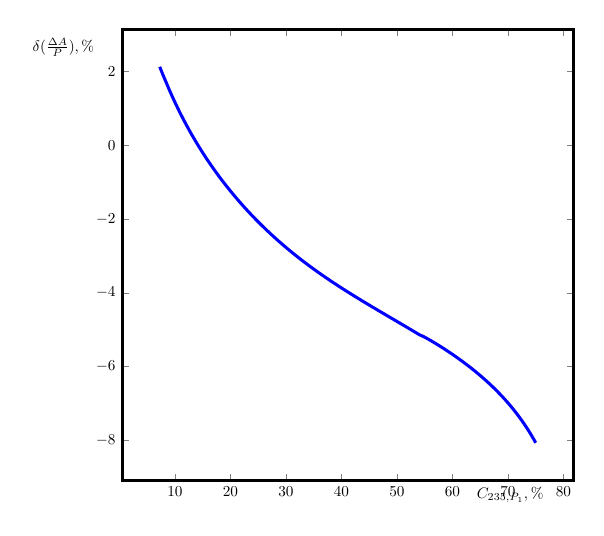
\begin{tikzpicture}[,
scale=0.55]
\begin{axis}[
  xlabel style = {{at={(axis description cs:.86,0)}}},
  ylabel = {$\delta(\frac{\Delta A}{P}), \%$},
  ylabel style = {{at={(axis description cs:-0.13,.925)},rotate=270,anchor=south}},
  xlabel = {$C_{235,P_1}, \%$},
  width=12cm, height=12cm, line width=2pt
]

\addplot+[
  mark = {none}
] coordinates {
  (7.249999999999999, 2.1301847994983807)
  (7.5, 2.0356830253537463)
  (7.75, 1.9423952267988522)
  (9.0, 1.4964966942451763)
  (9.25, 1.411600182824018)
  (9.5, 1.328130799140615)
  (9.75, 1.2460704008322467)
  (10.0, 1.1653880246172854)
  (10.25, 1.0860873850390034)
  (10.5, 1.0081092706387007)
  (10.75, 0.9314349174239751)
  (11.0, 0.8560332044167592)
  (11.25, 0.7818695828079755)
  (11.5, 0.7089181524016949)
  (11.75, 0.6371436734398068)
  (12.0, 0.5665138687079242)
  (12.25, 0.49699808926888195)
  (12.5, 0.4285644542996366)
  (12.75, 0.3611851855084861)
  (13.0, 0.2948268783690134)
  (13.25, 0.229463256791467)
  (13.5, 0.1650648557865053)
  (13.750000000000002, 0.1016073981819338)
  (14.000000000000002, 0.03906177065901577)
  (14.249999999999998, -0.022609469193761358)
  (14.499999999999998, -0.08340528533314681)
  (14.75, -0.1433606758886973)
  (15.0, -0.20249913496227764)
  (15.25, -0.26084285531180385)
  (15.5, -0.3184127258669716)
  (15.75, -0.3752287599350953)
  (16.0, -0.43131142223056346)
  (16.25, -0.48667854858529386)
  (16.5, -0.5413483836512691)
  (16.75, -0.5953391382375675)
  (17.0, -0.6486658752635573)
  (17.25, -0.7013461016024294)
  (17.5, -0.7533947037474772)
  (17.75, -0.8048248709819159)
  (18.0, -0.8556542122899644)
  (18.25, -0.9058964621272616)
  (18.5, -0.9555615277452705)
  (18.75, -1.0046636522718508)
  (19.0, -1.0532147373218788)
  (19.25, -1.1012270873585996)
  (19.5, -1.1487115295142003)
  (19.75, -1.1956791365615957)
  (20.0, -1.2421401505413958)
  (20.25, -1.2881052307853995)
  (20.5, -1.3335838930969208)
  (20.75, -1.3785844129009814)
  (21.0, -1.423117443498156)
  (21.25, -1.467190563396971)
  (21.5, -1.5108129725480375)
  (21.75, -1.5539920605167583)
  (22.0, -1.5967361800391118)
  (22.25, -1.6390525133748006)
  (22.5, -1.6809490068154944)
  (22.75, -1.7224323891003448)
  (23.0, -1.763509824744219)
  (23.25, -1.8041870698612077)
  (23.5, -1.8444714970912848)
  (23.75, -1.884369460995261)
  (24.0, -1.9238869894235648)
  (24.25, -1.963028794045824)
  (24.5, -2.001802998959367)
  (24.75, -2.0402132686905623)
  (25.0, -2.0782663125355434)
  (25.25, -2.1159653268245937)
  (25.5, -2.1533200126844134)
  (25.75, -2.1903299015202515)
  (26.0, -2.2270044524217805)
  (26.25, -2.2633473829825834)
  (26.5, -2.299362230452263)
  (26.75, -2.3350540083587665)
  (27.0, -2.3704287054636226)
  (27.250000000000004, -2.4054898637716353)
  (27.500000000000004, -2.4402421822092495)
  (27.750000000000004, -2.474689990856239)
  (28.000000000000004, -2.5088377969953264)
  (28.249999999999996, -2.5426893552478598)
  (28.499999999999996, -2.5762490154624507)
  (28.749999999999996, -2.609522452886624)
  (28.999999999999996, -2.6425118988066747)
  (29.25, -2.6752225234067515)
  (29.5, -2.707657609920724)
  (29.75, -2.7398216164072884)
  (30.0, -2.771717718276087)
  (30.25, -2.803351113359984)
  (30.5, -2.8347259226882007)
  (30.75, -2.8658444447808575)
  (31.0, -2.896711513380437)
  (31.25, -2.9273305447978895)
  (31.5, -2.9577052598003672)
  (31.75, -2.987840713528936)
  (32.0, -3.0177385405259556)
  (32.25, -3.0474046316963985)
  (32.5, -3.0768408990160787)
  (32.75, -3.1060531527140154)
  (33.0, -3.1350427562164627)
  (33.25, -3.163815129162785)
  (33.5, -3.1923723240006767)
  (33.75, -3.2207202733557394)
  (34.0, -3.2488605462044204)
  (34.25, -3.2767978440577745)
  (34.5, -3.3045352416846265)
  (34.75, -3.3320765520305584)
  (35.0, -3.3594263044809587)
  (35.25, -3.3865863444162545)
  (35.5, -3.413561804369768)
  (35.75, -3.4403556505588044)
  (36.0, -3.466971512854702)
  (36.25, -3.493412835386464)
  (36.5, -3.519683921806258)
  (36.75, -3.545787739494946)
  (37.0, -3.5717273090325388)
  (37.25, -3.59750740783894)
  (37.5, -3.6231301867534538)
  (37.75, -3.6486005742773853)
  (38.0, -3.67392108484207)
  (38.25, -3.6990955005792845)
  (38.5, -3.724127514805346)
  (38.75, -3.7490202178874577)
  (39.0, -3.7737778295476505)
  (39.25, -3.798403150311206)
  (39.5, -3.8228998089554467)
  (39.75, -3.847271518587854)
  (40.0, -3.8715220554781435)
  (40.25, -3.89565344153592)
  (40.5, -3.9196703593664117)
  (40.75, -3.9435762133355485)
  (41.0, -3.967373818353371)
  (41.25, -3.9910671973044862)
  (41.5, -4.014659033856855)
  (41.75, -4.038153165435792)
  (42.0, -4.061552668216013)
  (42.25, -4.0848613351327305)
  (42.5, -4.108082623108748)
  (42.75, -4.1312186739851455)
  (43.0, -4.154274742783619)
  (43.25, -4.177252586830833)
  (43.5, -4.20015616717915)
  (43.75, -4.22298840594045)
  (44.0, -4.245752835157836)
  (44.25, -4.268452956858278)
  (44.5, -4.29109151864581)
  (44.75, -4.313672043700648)
  (45.0, -4.3361979982287275)
  (45.25, -4.3586723527485605)
  (45.5, -4.381098535637343)
  (45.75, -4.403479502301739)
  (46.0, -4.4258187154230475)
  (46.25, -4.44811940848751)
  (46.5, -4.470384636603265)
  (46.75, -4.49261776029345)
  (47.0, -4.514821950026141)
  (47.25, -4.537000355114986)
  (47.5, -4.559156158477741)
  (47.75, -4.5812926466288415)
  (48.0, -4.6034131080592395)
  (48.25, -4.625520671535933)
  (48.5, -4.647618345481612)
  (48.75, -4.669709568790252)
  (49.0, -4.6917974706721965)
  (49.25, -4.713885367085347)
  (49.5, -4.735976393692837)
  (49.75, -4.758073833428612)
  (50.0, -4.780180707827004)
  (50.24999999999999, -4.80230068452831)
  (50.5, -4.8244368594909215)
  (50.74999999999999, -4.846592420941599)
  (51.0, -4.868770809714995)
  (51.24999999999999, -4.890975253295133)
  (51.5, -4.913209054605675)
  (51.74999999999999, -4.935475689146282)
  (52.0, -4.957778509003994)
  (52.25, -4.980120915177687)
  (52.5, -5.002506378710245)
  (52.75, -5.024938334102361)
  (53.0, -5.047420278857174)
  (53.25, -5.069955803112086)
  (53.5, -5.092548441935421)
  (53.75, -5.115201852668075)
  (54.0, -5.137919684231521)
  (54.25, -5.156459247876782)
  (54.50000000000001, -5.170099262405221)
  (54.75, -5.1882990426691284)
  (55.00000000000001, -5.207817874249847)
  (55.25, -5.2281041538907935)
  (55.50000000000001, -5.248937649768724)
  (55.75, -5.27020492338633)
  (56.00000000000001, -5.29183928315376)
  (56.25, -5.313798249593259)
  (56.49999999999999, -5.336053343953175)
  (56.75, -5.358584847345773)
  (56.99999999999999, -5.381378859974681)
  (57.25, -5.404425536147398)
  (57.49999999999999, -5.427717967767507)
  (57.75, -5.45125144763313)
  (57.99999999999999, -5.475022966325344)
  (58.25, -5.499030858718227)
  (58.5, -5.5232745451373075)
  (58.75, -5.547754365305986)
  (59.0, -5.5724714039344585)
  (59.25, -5.597427413626279)
  (59.5, -5.622624725944246)
  (59.75, -5.648066190027146)
  (60.0, -5.673755125251626)
  (60.25, -5.699695284748057)
  (60.5, -5.725890827433197)
  (60.75000000000001, -5.7523462968265555)
  (61.0, -5.7790666053499296)
  (61.25000000000001, -5.80605702312969)
  (61.5, -5.833322187818492)
  (61.75000000000001, -5.860870379278885)
  (62.0, -5.8887064614771765)
  (62.25000000000001, -5.916837126777856)
  (62.5, -5.945269405385256)
  (62.74999999999999, -5.974010673073261)
  (63.0, -6.0030686600143035)
  (63.24999999999999, -6.032451460754289)
  (63.5, -6.062167545381686)
  (63.74999999999999, -6.092225771935448)
  (64.0, -6.122635400103275)
  (64.25, -6.15340610626059)
  (64.5, -6.184547999912544)
  (64.75, -6.216071641598952)
  (65.0, -6.247988062339932)
  (65.25, -6.280308784696769)
  (65.5, -6.313045845541336)
  (65.75, -6.346211820633106)
  (66.0, -6.3798198511123925)
  (66.25, -6.413883672034067)
  (66.5, -6.448417643079258)
  (66.75, -6.4834367815921805)
  (67.0, -6.518956798112617)
  (67.25, -6.5549941345854315)
  (67.5, -6.591566005453064)
  (67.75, -6.628690441854883)
  (68.0, -6.66638633918127)
  (68.25, -6.704673508258825)
  (68.5, -6.743572730467931)
  (68.75, -6.783105817128049)
  (69.0, -6.823295673521218)
  (69.25, -6.864166367961815)
  (69.5, -6.905743206364523)
  (69.75, -6.948052812810802)
  (70.0, -6.991123216665509)
  (70.25, -7.034983946856116)
  (70.5, -7.07966613398926)
  (70.75, -7.1252026210547825)
  (71.0, -7.171628083540512)
  (71.25, -7.218980027250168)
  (71.5, -7.267295920133883)
  (71.75, -7.316617364665312)
  (72.0, -7.366987857543507)
  (72.25, -7.418453526273113)
  (72.5, -7.471063334717254)
  (72.75, -7.524869308552606)
  (73.0, -7.579926782925642)
  (73.25, -7.636294674912329)
  (73.5, -7.694035783750359)
  (73.75, -7.753217122216369)
  (74.0, -7.8139102830118174)
  (74.25, -7.8761918445719195)
  (74.5, -7.940143821368643)
  (74.75, -8.005854164539986)
  (75.0, -8.073417319568604)
};

\end{axis}
\end{tikzpicture}


\caption{{Зависимость экономии работы разделения в модифицированном двойном каскаде от концентрации $^{235}$U в потоке легкой фракции каскада I ($P_1$){\label{SW_lP1}}}}
    \end{minipage}
\end{figure}

\begin{figure}[ht]
    \centering
    \begin{minipage}{.5\textwidth}
        \centering
        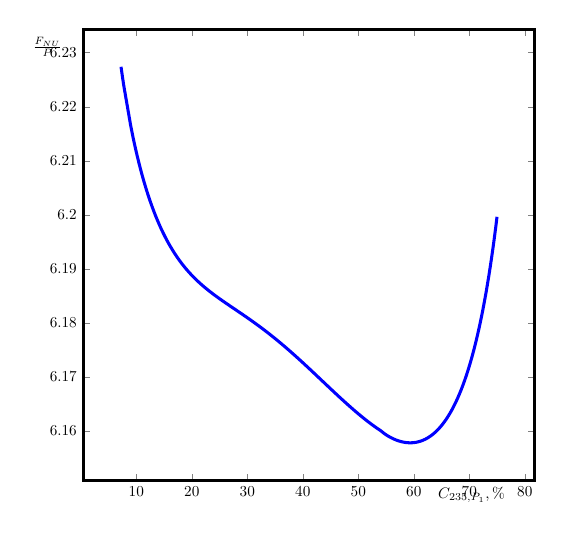
\begin{tikzpicture}[,
scale=0.55]
\begin{axis}[
  xlabel style = {{at={(axis description cs:.86,0)}}},
  ylabel = {$\frac{F_{NU}}{P}$},
  ylabel style = {{at={(axis description cs:-0.08,.925)},rotate=270,anchor=south}},
  xlabel = {$C_{235,P_1}, \%$},
  width=12cm, height=12cm, line width=2pt
]

\addplot+[
  mark = {none}
] coordinates {
  (7.249999999999999, 6.227377014019269)
  (7.5, 6.225574288089755)
  (7.75, 6.223861759784345)
  (9.0, 6.2164437851369865)
  (9.25, 6.215155377151255)
  (9.5, 6.213922740049087)
  (9.75, 6.212742643847732)
  (10.0, 6.211612001187144)
  (10.25, 6.210528387060725)
  (10.5, 6.209488912231413)
  (10.75, 6.208491358882763)
  (11.0, 6.207533563167729)
  (11.25, 6.206613463155888)
  (11.5, 6.20572926834755)
  (11.75, 6.204879205373501)
  (12.0, 6.204061666008173)
  (12.25, 6.203275092419443)
  (12.5, 6.202518099192422)
  (12.75, 6.201789235295246)
  (13.0, 6.201087410197339)
  (13.25, 6.200411324855954)
  (13.5, 6.199759924480936)
  (13.750000000000002, 6.199132021004566)
  (14.000000000000002, 6.198526738911426)
  (14.249999999999998, 6.197942913950563)
  (14.499999999999998, 6.197379984053495)
  (14.75, 6.196836858303185)
  (15.0, 6.196312745004527)
  (15.25, 6.195806870978311)
  (15.5, 6.195318474633009)
  (15.75, 6.194846822488212)
  (16.0, 6.194391268358382)
  (16.25, 6.193951106385381)
  (16.5, 6.193525708370521)
  (16.75, 6.19311450373791)
  (17.0, 6.192716827728326)
  (17.25, 6.192332180749601)
  (17.5, 6.191959992873057)
  (17.75, 6.191599747900141)
  (18.0, 6.191250921397608)
  (18.25, 6.190913003336374)
  (18.5, 6.190585562735798)
  (18.75, 6.190268115911817)
  (19.0, 6.189960203491246)
  (19.25, 6.189661419849706)
  (19.5, 6.189371323417035)
  (19.75, 6.189089518138411)
  (20.0, 6.1888155982901045)
  (20.25, 6.188549210396038)
  (20.5, 6.18828997271783)
  (20.75, 6.18803746988048)
  (21.0, 6.187791433961628)
  (21.25, 6.187551466011119)
  (21.5, 6.187317276163371)
  (21.75, 6.187088505078329)
  (22.0, 6.186864867245233)
  (22.25, 6.186646038114785)
  (22.5, 6.186431754359882)
  (22.75, 6.186221709413739)
  (23.0, 6.186015641436327)
  (23.25, 6.185813231164855)
  (23.5, 6.185614266284216)
  (23.75, 6.185418493153746)
  (24.0, 6.185225663271528)
  (24.25, 6.1850354723086145)
  (24.5, 6.184847812187333)
  (24.75, 6.18466235600372)
  (25.0, 6.184478950635638)
  (25.25, 6.184297272573964)
  (25.5, 6.184117354470624)
  (25.75, 6.18393870633129)
  (26.0, 6.183761376455242)
  (26.25, 6.183585115650957)
  (26.5, 6.183409684299104)
  (26.75, 6.183234954840314)
  (27.0, 6.1830607782895965)
  (27.250000000000004, 6.182886983991855)
  (27.500000000000004, 6.182713428725545)
  (27.750000000000004, 6.18253996996093)
  (28.000000000000004, 6.182366469888717)
  (28.249999999999996, 6.182192778097942)
  (28.499999999999996, 6.182018773824749)
  (28.749999999999996, 6.181844419098658)
  (28.999999999999996, 6.181669499803373)
  (29.25, 6.181493963074289)
  (29.5, 6.181317676559554)
  (29.75, 6.18114056396375)
  (30.0, 6.180962493842141)
  (30.25, 6.18078344854149)
  (30.5, 6.180603362214144)
  (30.75, 6.18042207616068)
  (31.0, 6.18023957507566)
  (31.25, 6.180055773753412)
  (31.5, 6.179870609574602)
  (31.75, 6.1796840986806965)
  (32.0, 6.179496076913787)
  (32.25, 6.179306618266495)
  (32.5, 6.179115583910541)
  (32.75, 6.178923054063513)
  (33.0, 6.17872887265614)
  (33.25, 6.178533107674346)
  (33.5, 6.178335650128213)
  (33.75, 6.178136607146121)
  (34.0, 6.177935851591383)
  (34.25, 6.177733433348179)
  (34.5, 6.177529315308404)
  (34.75, 6.177323509408283)
  (35.0, 6.177116065276798)
  (35.25, 6.17690689396963)
  (35.5, 6.1766960905810215)
  (35.75, 6.176483632144029)
  (36.0, 6.176269538038834)
  (36.25, 6.176053819751745)
  (36.5, 6.1758365430679305)
  (36.75, 6.175617698281583)
  (37.0, 6.175397285210312)
  (37.25, 6.175175404173838)
  (37.5, 6.174952011240878)
  (37.75, 6.174727220576204)
  (38.0, 6.174501016530132)
  (38.25, 6.174273454439577)
  (38.5, 6.174044590384136)
  (38.75, 6.173814445827527)
  (39.0, 6.173583110424997)
  (39.25, 6.173350596756331)
  (39.5, 6.173116966598365)
  (39.75, 6.172882287482483)
  (40.0, 6.172646632982597)
  (40.25, 6.172409981403761)
  (40.5, 6.172172463351168)
  (40.75, 6.171934137711886)
  (41.0, 6.1716950340774375)
  (41.25, 6.1714552494525154)
  (41.5, 6.171214809935404)
  (41.75, 6.170973808431834)
  (42.0, 6.1707322952533366)
  (42.25, 6.170490363571541)
  (42.5, 6.170248089766359)
  (42.75, 6.170005476408302)
  (43.0, 6.169762704615954)
  (43.25, 6.169519758904259)
  (43.5, 6.1692767499655305)
  (43.75, 6.1690337303599465)
  (44.0, 6.168790790272976)
  (44.25, 6.168548017894576)
  (44.5, 6.168305460973284)
  (44.75, 6.1680632121103915)
  (45.0, 6.167821359891942)
  (45.25, 6.167579970543602)
  (45.5, 6.167339132928801)
  (45.75, 6.167098911546122)
  (46.0, 6.16685940142854)
  (46.25, 6.166620684738383)
  (46.5, 6.1663828348847884)
  (46.75, 6.1661459422424745)
  (47.0, 6.165910089614895)
  (47.25, 6.165675356061189)
  (47.5, 6.165441826829726)
  (47.75, 6.165209591147368)
  (48.0, 6.164978740074744)
  (48.25, 6.164749355900007)
  (48.5, 6.1645215159278886)
  (48.75, 6.164295318848312)
  (49.0, 6.164070851398464)
  (49.25, 6.163848206277286)
  (49.5, 6.16362747116881)
  (49.75, 6.163408737437808)
  (50.0, 6.1631920873890325)
  (50.24999999999999, 6.16297763559227)
  (50.5, 6.162765466262529)
  (50.74999999999999, 6.162555670095732)
  (51.0, 6.1623483511216435)
  (51.24999999999999, 6.1621436022874025)
  (51.5, 6.161941519183411)
  (51.74999999999999, 6.161742209291162)
  (52.0, 6.16154577295669)
  (52.25, 6.161352311752986)
  (52.5, 6.161161932794009)
  (52.75, 6.16097474017067)
  (53.0, 6.160790841831792)
  (53.25, 6.160610351513262)
  (53.5, 6.160433378324685)
  (53.75, 6.160260039598731)
  (54.0, 6.160090450279548)
  (54.25, 6.159898234897805)
  (54.50000000000001, 6.159674341876738)
  (54.75, 6.159484660732906)
  (55.00000000000001, 6.159309726665361)
  (55.25, 6.159146291396782)
  (55.50000000000001, 6.158993118912496)
  (55.75, 6.1588496176370775)
  (56.00000000000001, 6.158715481018029)
  (56.25, 6.158590552287704)
  (56.49999999999999, 6.158474763282389)
  (56.75, 6.1583681031543795)
  (56.99999999999999, 6.158270600916357)
  (57.25, 6.158182315056757)
  (57.49999999999999, 6.158103327056908)
  (57.75, 6.158033737196367)
  (57.99999999999999, 6.157973661769213)
  (58.25, 6.157923231207986)
  (58.5, 6.157882588545942)
  (58.75, 6.157851889772119)
  (59.0, 6.157831301198988)
  (59.25, 6.157821000768727)
  (59.5, 6.157821177364845)
  (59.75, 6.157832030776999)
  (60.0, 6.157853771764251)
  (60.25, 6.157886622200484)
  (60.5, 6.157930815290082)
  (60.75000000000001, 6.157986595845348)
  (61.0, 6.158054220619495)
  (61.25000000000001, 6.158133958691122)
  (61.5, 6.158226031811696)
  (61.75000000000001, 6.158330876434335)
  (62.0, 6.158448713065213)
  (62.25000000000001, 6.1585798670675835)
  (62.5, 6.1587246781366165)
  (62.74999999999999, 6.158883501133261)
  (63.0, 6.159056706928311)
  (63.24999999999999, 6.159244683267737)
  (63.5, 6.1594478356689635)
  (63.74999999999999, 6.15966658835657)
  (64.0, 6.159901385245324)
  (64.25, 6.160152690977618)
  (64.5, 6.1604209920226225)
  (64.75, 6.160706797843675)
  (65.0, 6.161010642141147)
  (65.25, 6.161333084177535)
  (65.5, 6.161674710192321)
  (65.75, 6.162036134914214)
  (66.0, 6.162418003178991)
  (66.25, 6.1628209916616274)
  (66.5, 6.163245810732345)
  (66.75, 6.163693206446623)
  (67.0, 6.164163962680464)
  (67.25, 6.1646589034229695)
  (67.5, 6.165178895239631)
  (67.75, 6.165724849920823)
  (68.0, 6.166297727331531)
  (68.25, 6.16689853847998)
  (68.5, 6.167528348824437)
  (68.75, 6.168188281839634)
  (69.0, 6.168879522866356)
  (69.25, 6.169603323270165)
  (69.5, 6.17036100493807)
  (69.75, 6.171153965144866)
  (70.0, 6.171983681824327)
  (70.25, 6.172851719284132)
  (70.5, 6.173759734407551)
  (70.75, 6.174709483389582)
  (71.0, 6.175702829060102)
  (71.25, 6.1767418031952035)
  (71.5, 6.177828426904196)
  (71.75, 6.178964971159151)
  (72.0, 6.180153816804469)
  (72.25, 6.181397500356057)
  (72.5, 6.1826987266991384)
  (72.75, 6.184060383044718)
  (73.0, 6.185485554292268)
  (73.25, 6.186977539965906)
  (73.5, 6.188539872915019)
  (73.75, 6.190176339996345)
  (74.0, 6.191891004986476)
  (74.25, 6.193688234009228)
  (74.5, 6.1955727238049905)
  (74.75, 6.197549533218457)
  (75.0, 6.199624118338891)
};

\end{axis}
\end{tikzpicture}


  \caption{{Зависимость удельного расхода природного урана (безразмер.) от концентрации $^{235}$U в потоке легкой фракции первого каскада ($P_1$){\label{FnuP1}}}}
  \end{minipage}%
    \begin{minipage}{.5\textwidth}
      \centering
      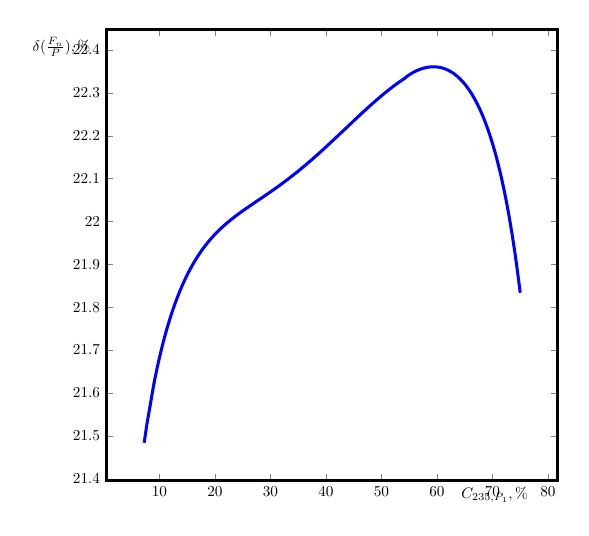
\begin{tikzpicture}[,
scale=0.55]
\begin{axis}[
  xlabel style = {{at={(axis description cs:.86,0)}}},
  ylabel = {$\delta(\frac{F_n}{P}), \%$},
  ylabel style = {{at={(axis description cs:-0.1,.925)},rotate=270,anchor=south}},
  xlabel = {$C_{235,P_1}, \%$},
  width=12cm, height=12cm, line width=2pt
]

\addplot+[
  mark = {none}
] coordinates {
  (7.249999999999999, 21.483689826405183)
  (7.5, 21.506419040955883)
  (7.75, 21.528011021545122)
  (9.0, 21.621538681258144)
  (9.25, 21.637783247920805)
  (9.5, 21.653324641484662)
  (9.75, 21.668203586371348)
  (10.0, 21.68245900878023)
  (10.25, 21.696121483794496)
  (10.5, 21.709227439629853)
  (10.75, 21.721804839064806)
  (11.0, 21.733880964418262)
  (11.25, 21.745481813019186)
  (11.5, 21.756629959930642)
  (11.75, 21.767347764230472)
  (12.0, 21.777655502824533)
  (12.25, 21.78757281724568)
  (12.5, 21.79711717514763)
  (12.75, 21.806306871499103)
  (13.0, 21.815155655979446)
  (13.25, 21.82367990724101)
  (13.5, 21.83189292433906)
  (13.750000000000002, 21.83980968672533)
  (14.000000000000002, 21.84744123311485)
  (14.249999999999998, 21.85480224267169)
  (14.499999999999998, 21.86189980209432)
  (14.75, 21.868747665934684)
  (15.0, 21.875355816080543)
  (15.25, 21.88173400096669)
  (15.5, 21.887891822927543)
  (15.75, 21.89383852986555)
  (16.0, 21.89958226904789)
  (16.25, 21.90513194010859)
  (16.5, 21.910495463532143)
  (16.75, 21.915680033280573)
  (17.0, 21.9206940308026)
  (17.25, 21.925543755079925)
  (17.5, 21.930236391914303)
  (17.75, 21.934778449664826)
  (18.0, 21.939176540515593)
  (18.25, 21.9434370950395)
  (18.5, 21.947565547147086)
  (18.75, 21.95156799524669)
  (19.0, 21.9554502312291)
  (19.25, 21.959217369306838)
  (19.5, 21.962874976905766)
  (19.75, 21.966428047583054)
  (20.0, 21.969881696803906)
  (20.25, 21.97324038128213)
  (20.5, 21.976508914069694)
  (20.75, 21.979692532317387)
  (21.0, 21.9827946140566)
  (21.25, 21.985820189349614)
  (21.5, 21.988772912893396)
  (21.75, 21.991657315336266)
  (22.0, 21.994476996468528)
  (22.25, 21.997236048288038)
  (22.5, 21.999937790888048)
  (22.75, 22.002586089538447)
  (23.0, 22.0051842455831)
  (23.25, 22.007736284366274)
  (23.5, 22.01024488280936)
  (23.75, 22.012713238876625)
  (24.0, 22.01514448574169)
  (24.25, 22.01754246045925)
  (24.5, 22.01990852569934)
  (24.75, 22.022246803147993)
  (25.0, 22.024559223407014)
  (25.25, 22.026849865359488)
  (25.5, 22.029118317321828)
  (25.75, 22.03137075726377)
  (26.0, 22.033606576216037)
  (26.25, 22.035828916046984)
  (26.5, 22.038040797936475)
  (26.75, 22.040243830184547)
  (27.0, 22.04243989123085)
  (27.250000000000004, 22.044631132737045)
  (27.500000000000004, 22.046819360475812)
  (27.750000000000004, 22.04900637149735)
  (28.000000000000004, 22.051193903335275)
  (28.249999999999996, 22.05338385240828)
  (28.499999999999996, 22.05557774133692)
  (28.749999999999996, 22.057776048862422)
  (28.999999999999996, 22.059981474615988)
  (29.25, 22.06219468512767)
  (29.5, 22.064417349122355)
  (29.75, 22.066650428551547)
  (30.0, 22.068895580702996)
  (30.25, 22.071153028153077)
  (30.5, 22.07342360112531)
  (30.75, 22.07570930054128)
  (31.0, 22.078010319375707)
  (31.25, 22.080327731922832)
  (31.5, 22.082662327702696)
  (31.75, 22.08501390319967)
  (32.0, 22.087384528157315)
  (32.25, 22.08977326965832)
  (32.5, 22.092181878084016)
  (32.75, 22.09460934203118)
  (33.0, 22.097057629259798)
  (33.25, 22.099525882586533)
  (33.5, 22.102015476183222)
  (33.75, 22.104525059348756)
  (34.0, 22.107056235053935)
  (34.25, 22.109608374346678)
  (34.5, 22.112181945095156)
  (34.75, 22.11477679680448)
  (35.0, 22.11739230374018)
  (35.25, 22.120029587334223)
  (35.5, 22.122687448614887)
  (35.75, 22.12536617715506)
  (36.0, 22.128065528604623)
  (36.25, 22.13078535814138)
  (36.5, 22.13352483632962)
  (36.75, 22.13628408554259)
  (37.0, 22.139063108079892)
  (37.25, 22.141860639085674)
  (37.5, 22.144677232456424)
  (37.75, 22.14751144877445)
  (38.0, 22.150363485354852)
  (38.25, 22.1532326444961)
  (38.5, 22.15611821913277)
  (38.75, 22.159019938644974)
  (39.0, 22.161936672637196)
  (39.25, 22.16486826250039)
  (39.5, 22.167813929336923)
  (39.75, 22.170772821694396)
  (40.0, 22.173744011934705)
  (40.25, 22.17672777359313)
  (40.5, 22.179722459967067)
  (40.75, 22.18272732859379)
  (41.0, 22.185742006376053)
  (41.25, 22.188765270254706)
  (41.5, 22.19179679117612)
  (41.75, 22.194835397761835)
  (42.0, 22.19788045567166)
  (42.25, 22.2009307901746)
  (42.5, 22.20398543825385)
  (42.75, 22.20704436749975)
  (43.0, 22.21010529432439)
  (43.25, 22.2131684139672)
  (43.5, 22.216232330792085)
  (43.75, 22.219296382107323)
  (44.0, 22.222359430832206)
  (44.25, 22.225420365045945)
  (44.5, 22.228478582723156)
  (44.75, 22.231532916323836)
  (45.0, 22.234582248933254)
  (45.25, 22.237625745561807)
  (45.5, 22.240662285797374)
  (45.75, 22.243691056425885)
  (46.0, 22.246710859248086)
  (46.25, 22.249720658340987)
  (46.5, 22.25271952814405)
  (46.75, 22.25570632919044)
  (47.0, 22.25868001747373)
  (47.25, 22.26163959619677)
  (47.5, 22.264583990526976)
  (47.75, 22.26751207547001)
  (48.0, 22.270422702910942)
  (48.25, 22.273314835340386)
  (48.5, 22.276187498081136)
  (48.75, 22.279039446826232)
  (49.0, 22.28186958797177)
  (49.25, 22.284676752746556)
  (49.5, 22.287459835608615)
  (49.75, 22.290217684608304)
  (50.0, 22.29294926202693)
  (50.24999999999999, 22.295653123340287)
  (50.5, 22.2983282067447)
  (50.74999999999999, 22.300973368723554)
  (51.0, 22.303587297643833)
  (51.24999999999999, 22.30616882160501)
  (51.5, 22.30871673537964)
  (51.74999999999999, 22.31122968381447)
  (52.0, 22.313706401721866)
  (52.25, 22.316145608444437)
  (52.5, 22.318545953462888)
  (52.75, 22.32090612437324)
  (53.0, 22.323224760130035)
  (53.25, 22.325500426723067)
  (53.5, 22.327731748471447)
  (53.75, 22.32991724601584)
  (54.0, 22.332055470111968)
  (54.25, 22.33447896920301)
  (54.50000000000001, 22.337301867808346)
  (54.75, 22.33969341460079)
  (55.00000000000001, 22.341899026606672)
  (55.25, 22.343959658910162)
  (55.50000000000001, 22.34589089549006)
  (55.75, 22.347700195075692)
  (56.00000000000001, 22.349391422756803)
  (56.25, 22.350966555098672)
  (56.49999999999999, 22.352426451526252)
  (56.75, 22.353771248810105)
  (56.99999999999999, 22.355000581151153)
  (57.25, 22.356113711112723)
  (57.49999999999999, 22.357109611358062)
  (57.75, 22.357987017537727)
  (57.99999999999999, 22.358744463387183)
  (58.25, 22.359380304380682)
  (58.5, 22.35989273711957)
  (58.75, 22.36027979485543)
  (59.0, 22.3605393806795)
  (59.25, 22.360669251052776)
  (59.5, 22.360667024485224)
  (59.75, 22.36053018197943)
  (60.0, 22.360256066232985)
  (60.25, 22.35984187980509)
  (60.5, 22.359284682397163)
  (60.75000000000001, 22.358581387355102)
  (61.0, 22.35772875747091)
  (61.25000000000001, 22.356723400135003)
  (61.5, 22.35556251945002)
  (61.75000000000001, 22.35424061250708)
  (62.0, 22.352754899109772)
  (62.25000000000001, 22.3511012769977)
  (62.5, 22.349275463210095)
  (62.74999999999999, 22.34727298357233)
  (63.0, 22.34508916205368)
  (63.24999999999999, 22.34271910985699)
  (63.5, 22.34015771411826)
  (63.74999999999999, 22.33739962610901)
  (64.0, 22.33443924884203)
  (64.25, 22.33127072399107)
  (64.5, 22.327887918032474)
  (64.75, 22.324284407526417)
  (65.0, 22.320453463446587)
  (65.25, 22.31638803447302)
  (65.5, 22.312080729153326)
  (65.75, 22.307523796835802)
  (66.0, 22.302709107271447)
  (66.25, 22.29762812877475)
  (66.5, 22.292271904822194)
  (66.75, 22.2866310289617)
  (67.0, 22.28069561789068)
  (67.25, 22.274455282550676)
  (67.5, 22.267899097069556)
  (67.75, 22.2610155653687)
  (68.0, 22.25379258523287)
  (68.25, 22.24621740962022)
  (68.5, 22.238276604969307)
  (68.75, 22.229956006232733)
  (69.0, 22.221240668340613)
  (69.25, 22.212114813766316)
  (69.5, 22.202561775831377)
  (69.75, 22.192563937349476)
  (70.0, 22.182102664165903)
  (70.25, 22.171158233102396)
  (70.5, 22.159709753764755)
  (70.75, 22.14773508361193)
  (71.0, 22.13521073562392)
  (71.25, 22.122111092665044)
  (71.5, 22.10841067208905)
  (71.75, 22.094080840918217)
  (72.0, 22.07909158087724)
  (72.25, 22.063410910946)
  (72.5, 22.047004727262333)
  (72.75, 22.02983662715554)
  (73.0, 22.011867715449828)
  (73.25, 21.993056390928732)
  (73.5, 21.9733581105531)
  (73.75, 21.952725128696205)
  (74.0, 21.931106208257333)
  (74.25, 21.90844630006714)
  (74.5, 21.884686186460733)
  (74.75, 21.85976208427254)
  (75.0, 21.833605201779182)
};

\end{axis}
\end{tikzpicture}


\caption{{Зависимость экономим природного урана от концентрации $^{235}$U в потоке легкой фракции первого каскада ($P_1$){\label{pFoP1}}}}
    \end{minipage}
\end{figure}


\begin{figure}[ht]
    \centering
    \begin{minipage}{.5\textwidth}
      \centering
      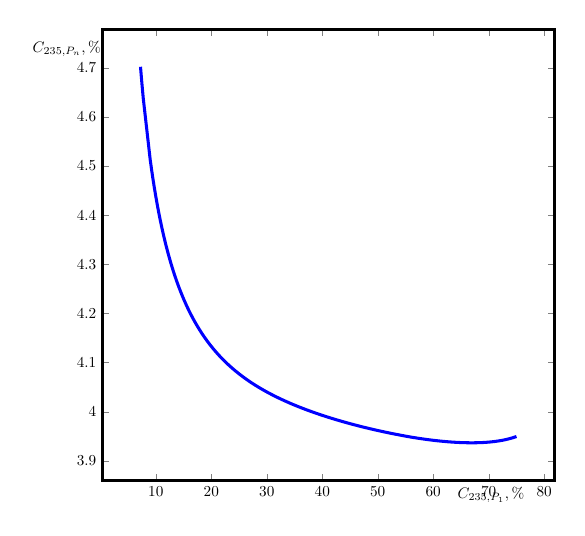
\begin{tikzpicture}[,
scale=0.55]
\begin{axis}[
  xlabel style = {{at={(axis description cs:.86,0)}}},
  ylabel = {$C_{235,P_n}, \%$},
  ylabel style = {{at={(axis description cs:-0.08,.925)},rotate=270,anchor=south}},
  xlabel = {$C_{235,P_1}, \%$},
  width=12cm, height=12cm, line width=2pt
]

\addplot+[
  mark = {none}
] coordinates {
  (7.249999999999999, 4.701988557469205)
  (7.5, 4.668419451766131)
  (7.75, 4.637445519842572)
  (9.0, 4.512656964243577)
  (9.25, 4.492392391665288)
  (9.5, 4.473358893808722)
  (9.75, 4.455447521722275)
  (10.0, 4.438561777842849)
  (10.25, 4.4226162163447755)
  (10.5, 4.407534264604589)
  (10.75, 4.393247736657043)
  (11.0, 4.379695404161248)
  (11.25, 4.366822153223248)
  (11.5, 4.354578348284348)
  (11.75, 4.342919031244304)
  (12.0, 4.331803468557111)
  (12.25, 4.32119460481474)
  (12.5, 4.3110587328198315)
  (12.75, 4.301364985015501)
  (13.0, 4.292085298371289)
  (13.25, 4.283193778015583)
  (13.5, 4.2746667512446)
  (13.750000000000002, 4.266482317334011)
  (14.000000000000002, 4.25862044888284)
  (14.249999999999998, 4.251062447338917)
  (14.499999999999998, 4.243791360677786)
  (14.75, 4.236791144875945)
  (15.0, 4.230047071290359)
  (15.25, 4.223545448096309)
  (15.5, 4.217273525380591)
  (15.75, 4.2112194244700225)
  (16.0, 4.205372102336546)
  (16.25, 4.199721193414945)
  (16.5, 4.194257037157774)
  (16.75, 4.188970611971359)
  (17.0, 4.183853391777843)
  (17.25, 4.178897465153345)
  (17.5, 4.1740953479622585)
  (17.75, 4.169440025087747)
  (18.0, 4.1649248794348415)
  (18.25, 4.160543675688258)
  (18.5, 4.156290573307494)
  (18.75, 4.152160020211794)
  (19.0, 4.148146777548833)
  (19.25, 4.14424591726013)
  (19.5, 4.140452747161554)
  (19.75, 4.136762844046728)
  (20.0, 4.133172003248815)
  (20.25, 4.129676262175772)
  (20.5, 4.126271836684657)
  (20.75, 4.122955105204843)
  (21.0, 4.11972270907863)
  (21.25, 4.1165713694744)
  (21.5, 4.113498025887383)
  (21.75, 4.110499716544544)
  (22.0, 4.107573658306183)
  (22.25, 4.104717169044741)
  (22.5, 4.101927722054008)
  (22.75, 4.099202874796242)
  (23.0, 4.096540316674312)
  (23.25, 4.0939378002303775)
  (23.5, 4.09139323663827)
  (23.75, 4.088904599339217)
  (24.0, 4.086469947765354)
  (24.25, 4.084087385441765)
  (24.5, 4.081755210341575)
  (24.75, 4.079471656350292)
  (25.0, 4.077235130296242)
  (25.25, 4.075043997580162)
  (25.5, 4.072896901274405)
  (25.75, 4.070792221215151)
  (26.0, 4.068728720283428)
  (26.25, 4.066705030394494)
  (26.5, 4.064719837855806)
  (26.75, 4.062771943513446)
  (27.0, 4.06086017901786)
  (27.250000000000004, 4.058983404417401)
  (27.500000000000004, 4.057140536263129)
  (27.750000000000004, 4.055330529343949)
  (28.000000000000004, 4.053552377395919)
  (28.249999999999996, 4.051805100839315)
  (28.499999999999996, 4.050087770956992)
  (28.749999999999996, 4.048399540691778)
  (28.999999999999996, 4.046739485640057)
  (29.25, 4.0451068080687795)
  (29.5, 4.0435006891248415)
  (29.75, 4.041920370108527)
  (30.0, 4.0403650837112535)
  (30.25, 4.038834155588793)
  (30.5, 4.037326904888013)
  (30.75, 4.035842616233084)
  (31.0, 4.034380682212641)
  (31.25, 4.03294047301185)
  (31.5, 4.031521391722611)
  (31.75, 4.030122907581362)
  (32.0, 4.028744398176003)
  (32.25, 4.027385402369926)
  (32.5, 4.026045346316909)
  (32.75, 4.024723804453619)
  (33.0, 4.023420223104561)
  (33.25, 4.022134198651417)
  (33.5, 4.020865234180913)
  (33.75, 4.0196129768377356)
  (34.0, 4.01837694482804)
  (34.25, 4.017156775727496)
  (34.5, 4.0159520663383095)
  (34.75, 4.014762454488629)
  (35.0, 4.013587611740333)
  (35.25, 4.012427136485997)
  (35.5, 4.011280748454745)
  (35.75, 4.010148105864053)
  (36.0, 4.0090289019419005)
  (36.25, 4.007922834254498)
  (36.5, 4.006829641893421)
  (36.75, 4.00574902687503)
  (37.0, 4.004680705133545)
  (37.25, 4.003624461083854)
  (37.5, 4.002579999774173)
  (37.75, 4.00154712889979)
  (38.0, 4.00052558499739)
  (38.25, 3.999515154245043)
  (38.5, 3.998515629873292)
  (38.75, 3.9975267906700376)
  (39.0, 3.9965484626630916)
  (39.25, 3.9955804314500236)
  (39.5, 3.9946225180316963)
  (39.75, 3.993674552463375)
  (40.0, 3.9927363738403554)
  (40.25, 3.9918077691848497)
  (40.5, 3.9908886222047335)
  (40.75, 3.989978778370499)
  (41.0, 3.989078070289957)
  (41.25, 3.988186375711534)
  (41.5, 3.9873035342115206)
  (41.75, 3.986429429842854)
  (42.0, 3.9855639252503536)
  (42.25, 3.984706912886249)
  (42.5, 3.9838582790425194)
  (42.75, 3.9830178695069356)
  (43.0, 3.982185640986527)
  (43.25, 3.981361435720606)
  (43.5, 3.9805451751944934)
  (43.75, 3.9797367493765425)
  (44.0, 3.97893607409464)
  (44.25, 3.9781430671633604)
  (44.5, 3.9773576252232643)
  (44.75, 3.976579674829628)
  (45.0, 3.975809143046644)
  (45.25, 3.975045946347608)
  (45.5, 3.9742900175468057)
  (45.75, 3.9735412775206225)
  (46.0, 3.972799668049243)
  (46.25, 3.972065125724179)
  (46.5, 3.971337584346804)
  (46.75, 3.970616990278185)
  (47.0, 3.9699032876572353)
  (47.25, 3.9691964206491273)
  (47.5, 3.9684963393147763)
  (47.75, 3.967802998243279)
  (48.0, 3.967116355198091)
  (48.25, 3.9664363647146823)
  (48.5, 3.965762980313272)
  (48.75, 3.965096170246839)
  (49.0, 3.9644358974637224)
  (49.25, 3.96378213031457)
  (49.5, 3.9631348359046443)
  (49.75, 3.9624939852823746)
  (50.0, 3.961859545739176)
  (50.24999999999999, 3.9612315055208818)
  (50.5, 3.960609836300489)
  (50.74999999999999, 3.9599945151799614)
  (51.0, 3.959385528753841)
  (51.24999999999999, 3.9587828584606313)
  (51.5, 3.958186488764011)
  (51.74999999999999, 3.9575964126327863)
  (52.0, 3.9570126201357745)
  (52.25, 3.956435103412865)
  (52.5, 3.9558638592099777)
  (52.75, 3.955298883735607)
  (53.0, 3.9547401767382864)
  (53.25, 3.95418774262707)
  (53.5, 3.953641584225888)
  (53.75, 3.953101710413117)
  (54.0, 3.952568129763514)
  (54.25, 3.9520242386043596)
  (54.50000000000001, 3.9514638938443376)
  (54.75, 3.9509286093313047)
  (55.00000000000001, 3.9504061518382803)
  (55.25, 3.949894431346647)
  (55.50000000000001, 3.9493926169099254)
  (55.75, 3.948900281560302)
  (56.00000000000001, 3.948417177414651)
  (56.25, 3.947943151049153)
  (56.49999999999999, 3.947478105199625)
  (56.75, 3.947021979160744)
  (56.99999999999999, 3.9465747378380307)
  (57.25, 3.946136365223269)
  (57.49999999999999, 3.945706860310912)
  (57.75, 3.94528623444606)
  (57.99999999999999, 3.9448745095552176)
  (58.25, 3.9444717169449057)
  (58.5, 3.944077896319619)
  (58.75, 3.943693095941572)
  (59.0, 3.943317371015641)
  (59.25, 3.9429507844314884)
  (59.5, 3.942593406319508)
  (59.75, 3.94224531400009)
  (60.0, 3.941906591994261)
  (60.25, 3.941577332085386)
  (60.5, 3.941257633424412)
  (60.75000000000001, 3.9409476026732304)
  (61.0, 3.9406473541822398)
  (61.25000000000001, 3.940357010199449)
  (61.5, 3.9400766653004426)
  (61.75000000000001, 3.9398065425317914)
  (62.0, 3.9395467367324444)
  (62.25000000000001, 3.9392974057156938)
  (62.5, 3.9390587162960835)
  (62.74999999999999, 3.938830844769181)
  (63.0, 3.9386139773975497)
  (63.24999999999999, 3.9384083109094754)
  (63.5, 3.93821405301616)
  (63.74999999999999, 3.9380314229524163)
  (64.0, 3.9378606520455084)
  (64.25, 3.9377019843163357)
  (64.5, 3.9375556771172384)
  (64.75, 3.937422001810298)
  (65.0, 3.9373012444903743)
  (65.25, 3.9371937067568585)
  (65.5, 3.9370997065385755)
  (65.75, 3.937019578976327)
  (66.0, 3.9369536773678977)
  (66.25, 3.936902374180637)
  (66.5, 3.9368660621373093)
  (66.75, 3.936845155381072)
  (67.0, 3.9368400907262826)
  (67.25, 3.9368513290022)
  (67.5, 3.9368793564974567)
  (67.75, 3.9369246865138763)
  (68.0, 3.9369878610390243)
  (68.25, 3.9370694525479206)
  (68.5, 3.93717006594525)
  (68.75, 3.9372903406607054)
  (69.0, 3.937430952911299)
  (69.25, 3.93759261814597)
  (69.5, 3.937776093689399)
  (69.75, 3.937982181603758)
  (70.0, 3.9382117317890457)
  (70.25, 3.9384656453449436)
  (70.5, 3.9387448782194703)
  (70.75, 3.939050445172535)
  (71.0, 3.9393834240852863)
  (71.25, 3.9397449929659283)
  (71.5, 3.9401363230673376)
  (71.75, 3.9405587338003687)
  (72.0, 3.941013609388027)
  (72.25, 3.941502426041414)
  (72.5, 3.9420267594351284)
  (72.75, 3.9425882929237814)
  (73.0, 3.9431888265864643)
  (73.25, 3.9438302871975597)
  (73.5, 3.9445147392362023)
  (73.75, 3.945244397062038)
  (74.0, 3.9460216384036566)
  (74.25, 3.9468490193269803)
  (74.5, 3.9477292908758947)
  (74.75, 3.9486654176063984)
  (75.0, 3.9496605982694417)
};

\end{axis}
\end{tikzpicture}


\caption{{Зависимость концентрации $^{235}$U в НОУ-разбавителе от концентрации $^{235}$U в потоке легкой фракции первого каскада ($P_1$){\label{C235P0}}}}
\end{minipage}
\end{figure}

\begin{figure}[ht]
    \centering
    \begin{minipage}{.5\textwidth}
      \centering
      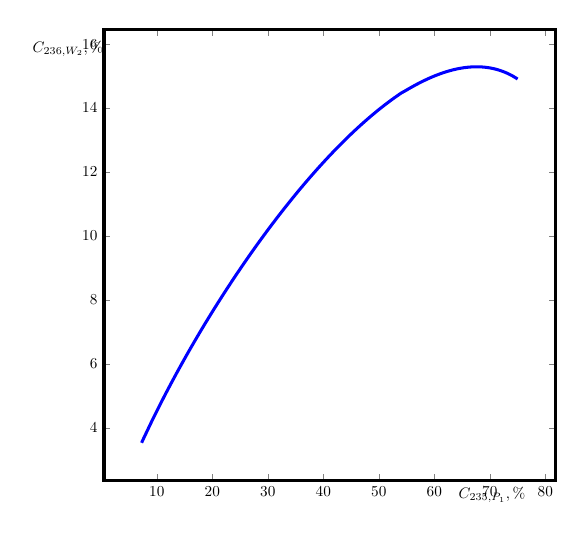
\begin{tikzpicture}[,
scale=0.55]
\begin{axis}[
  xlabel style = {{at={(axis description cs:.86,0)}}},
  ylabel = {$C_{236,W_2}, \%$},
  ylabel style = {{at={(axis description cs:-0.08,.925)},rotate=270,anchor=south}},
  xlabel = {$C_{235,P_1}, \%$},
  width=12cm, height=12cm, line width=2pt
]

\addplot+[
  mark = {none}
] coordinates {
  (7.249999999999999, 3.5342592482941146)
  (7.5, 3.628274808507897)
  (7.75, 3.7215030870706745)
  (9.0, 4.176686672127894)
  (9.25, 4.265680830565658)
  (9.5, 4.354037829781733)
  (9.75, 4.441774219059031)
  (10.0, 4.5289058522938905)
  (10.25, 4.615446741312886)
  (10.5, 4.7014116788889515)
  (10.75, 4.786813628110336)
  (11.0, 4.871665162524931)
  (11.25, 4.955978315813709)
  (11.5, 5.039764270870576)
  (11.75, 5.123033926334003)
  (12.0, 5.205797586284634)
  (12.25, 5.288065079776838)
  (12.5, 5.369845789301893)
  (12.75, 5.451148678397203)
  (13.0, 5.531982319398478)
  (13.25, 5.6123549125954755)
  (13.5, 5.692274313315904)
  (13.750000000000002, 5.771748041407735)
  (14.000000000000002, 5.85078331563655)
  (14.249999999999998, 5.929387479205129)
  (14.499999999999998, 6.007566340779183)
  (14.75, 6.085326686010806)
  (15.0, 6.162674647461732)
  (15.25, 6.239616117120433)
  (15.5, 6.316156759453867)
  (15.75, 6.392302022924749)
  (16.0, 6.468057157359188)
  (16.25, 6.543427205925685)
  (16.5, 6.618417032088765)
  (16.75, 6.69303132401534)
  (17.0, 6.767274580104984)
  (17.25, 6.84115116118502)
  (17.5, 6.914665250622311)
  (17.75, 6.987820834343957)
  (18.0, 7.060621912669937)
  (18.25, 7.133072250591871)
  (18.5, 7.205175348275931)
  (18.75, 7.276934754531787)
  (19.0, 7.348353830470784)
  (19.25, 7.419435830969122)
  (19.5, 7.490183879892035)
  (19.75, 7.560600997513528)
  (20.0, 7.630690090671088)
  (20.25, 7.70045397219576)
  (20.5, 7.769895343828)
  (20.75, 7.8390167930675565)
  (21.0, 7.907820854601059)
  (21.25, 7.97630992961601)
  (21.5, 8.04448635867453)
  (21.75, 8.112352371160432)
  (22.0, 8.179910131430894)
  (22.25, 8.247161707019421)
  (22.5, 8.314109104608551)
  (22.75, 8.380754235798818)
  (23.0, 8.447098945885584)
  (23.25, 8.5131449858254)
  (23.5, 8.57889406681402)
  (23.75, 8.644347823909717)
  (24.0, 8.709507811209303)
  (24.25, 8.77437549207649)
  (24.5, 8.838952354546205)
  (24.75, 8.903239711829398)
  (25.0, 8.96723890180032)
  (25.25, 9.030951105494324)
  (25.5, 9.094377641422094)
  (25.75, 9.157519468633817)
  (26.0, 9.22037779576328)
  (26.25, 9.282953609644245)
  (26.5, 9.345247829925137)
  (26.75, 9.407261376391864)
  (27.0, 9.468995163952169)
  (27.250000000000004, 9.53044996608274)
  (27.500000000000004, 9.591626557288091)
  (27.750000000000004, 9.652525646860372)
  (28.000000000000004, 9.713147915089403)
  (28.249999999999996, 9.773493964598734)
  (28.499999999999996, 9.833564379636996)
  (28.749999999999996, 9.893359762244833)
  (28.999999999999996, 9.952880523226241)
  (29.25, 10.01212716527943)
  (29.5, 10.071100065778172)
  (29.75, 10.129799616755456)
  (30.0, 10.188226114146849)
  (30.25, 10.246379916196307)
  (30.5, 10.304261290710345)
  (30.75, 10.361870378988712)
  (31.0, 10.419207416740369)
  (31.25, 10.476272532169663)
  (31.5, 10.53306583562083)
  (31.75, 10.589587479744225)
  (32.0, 10.645837393747396)
  (32.25, 10.701815714130055)
  (32.5, 10.757522322008985)
  (32.75, 10.812957295691577)
  (33.0, 10.86812041170528)
  (33.25, 10.923011672456234)
  (33.5, 10.977630834263087)
  (33.75, 11.031977877657594)
  (34.0, 11.086052471474597)
  (34.25, 11.139854459492627)
  (34.5, 11.193383556699708)
  (34.75, 11.246639487400154)
  (35.0, 11.299622022051311)
  (35.25, 11.352330694540006)
  (35.5, 11.404765254073157)
  (35.75, 11.456925275434992)
  (36.0, 11.508810349809835)
  (36.25, 11.56042003352676)
  (36.5, 11.61175391552551)
  (36.75, 11.66281147285595)
  (37.0, 11.713592147969624)
  (37.25, 11.76409550552745)
  (37.5, 11.814320874072605)
  (37.75, 11.864267790371391)
  (38.0, 11.913935556826571)
  (38.25, 11.963323570017318)
  (38.5, 12.012431185981121)
  (38.75, 12.06125769749639)
  (39.0, 12.109802468655486)
  (39.25, 12.158064711152651)
  (39.5, 12.20604368835982)
  (39.75, 12.253738655884987)
  (40.0, 12.30114885406309)
  (40.25, 12.348273321808454)
  (40.5, 12.395111335671876)
  (40.75, 12.441662033289042)
  (41.0, 12.487924459646774)
  (41.25, 12.533897773083694)
  (41.5, 12.57958095678315)
  (41.75, 12.624973092926552)
  (42.0, 12.670073165221329)
  (42.25, 12.714880209770163)
  (42.5, 12.759393201133115)
  (42.75, 12.80361094357164)
  (43.0, 12.847532569846754)
  (43.25, 12.891156786627631)
  (43.5, 12.934482530646024)
  (43.75, 12.977508594627546)
  (44.0, 13.020233810259285)
  (44.25, 13.062656989057563)
  (44.5, 13.104776816766996)
  (44.75, 13.146592050098283)
  (45.0, 13.18810142298697)
  (45.25, 13.229303553944982)
  (45.5, 13.270197115208738)
  (45.75, 13.310780680224651)
  (46.0, 13.35105285668299)
  (46.25, 13.391012196465132)
  (46.5, 13.430657193393996)
  (46.75, 13.469986359238753)
  (47.0, 13.508998134355688)
  (47.25, 13.54769094165767)
  (47.5, 13.586063155503533)
  (47.75, 13.62411314618969)
  (48.0, 13.66183924409776)
  (48.25, 13.699239721963105)
  (48.5, 13.736312789278726)
  (48.75, 13.773056705621245)
  (49.0, 13.809469614243671)
  (49.25, 13.845549679192395)
  (49.5, 13.881294966603333)
  (49.75, 13.916703556029491)
  (50.0, 13.951773407993153)
  (50.24999999999999, 13.986502576157287)
  (50.5, 14.020888964268755)
  (50.74999999999999, 14.054930438510576)
  (51.0, 14.088624869162498)
  (51.24999999999999, 14.121970036326267)
  (51.5, 14.15496369515811)
  (51.74999999999999, 14.187603567668189)
  (52.0, 14.219887303342038)
  (52.25, 14.25181251758511)
  (52.5, 14.283376773057183)
  (52.75, 14.314577575506757)
  (53.0, 14.34541238179704)
  (53.25, 14.375878602167152)
  (53.5, 14.405973584806492)
  (53.75, 14.435694627828713)
  (54.0, 14.465038975318953)
  (54.25, 14.491510191679907)
  (54.50000000000001, 14.514251311378368)
  (54.75, 14.539120084382464)
  (55.00000000000001, 14.56425849780916)
  (55.25, 14.589349026309453)
  (55.50000000000001, 14.614262607673128)
  (55.75, 14.638930573247745)
  (56.00000000000001, 14.663310489095066)
  (56.25, 14.687373379948488)
  (56.49999999999999, 14.711097956576802)
  (56.75, 14.734467660368612)
  (56.99999999999999, 14.75746900818406)
  (57.25, 14.780090600144542)
  (57.49999999999999, 14.80232249205738)
  (57.75, 14.824155780786047)
  (57.99999999999999, 14.845582320176067)
  (58.25, 14.866594520312045)
  (58.5, 14.88718520070624)
  (58.75, 14.907347486897066)
  (59.0, 14.927074719686779)
  (59.25, 14.9463603981486)
  (59.5, 14.96519812723627)
  (59.75, 14.983581577481905)
  (60.0, 15.00150445210187)
  (60.25, 15.018960459717787)
  (60.5, 15.035943291378953)
  (60.75000000000001, 15.052446600908281)
  (61.0, 15.068463987835184)
  (61.25000000000001, 15.0839889823528)
  (61.5, 15.099014805374708)
  (61.75000000000001, 15.113535342577142)
  (62.0, 15.127543506550948)
  (62.25000000000001, 15.141032435229555)
  (62.5, 15.15399513757708)
  (62.74999999999999, 15.166424484843704)
  (63.0, 15.178313201993351)
  (63.24999999999999, 15.189653859245233)
  (63.5, 15.200438863677679)
  (63.74999999999999, 15.210660450847218)
  (64.0, 15.22031067638054)
  (64.25, 15.229381407499712)
  (64.5, 15.237864314444655)
  (64.75, 15.245750861758259)
  (65.0, 15.253032299402117)
  (65.25, 15.259699653671186)
  (65.5, 15.26574371787803)
  (65.75, 15.271155042776577)
  (66.0, 15.275923926696949)
  (66.25, 15.280040405362172)
  (66.5, 15.283494241358284)
  (66.75, 15.286274913228507)
  (67.0, 15.288371604162187)
  (67.25, 15.289773190248196)
  (67.5, 15.290468228262103)
  (67.75, 15.290444942955173)
  (68.0, 15.289691213812196)
  (68.25, 15.288194561244081)
  (68.5, 15.285942132179251)
  (68.75, 15.28292068501691)
  (69.0, 15.279116573902577)
  (69.25, 15.27451573228486)
  (69.5, 15.269103655709834)
  (69.75, 15.26286538380682)
  (70.0, 15.25578548141617)
  (70.25, 15.247848018806613)
  (70.5, 15.239036550925361)
  (70.75, 15.229334095619915)
  (71.0, 15.218723110764426)
  (71.25, 15.20718571833361)
  (71.5, 15.194702805223118)
  (71.75, 15.181255176683559)
  (72.0, 15.166822813345304)
  (72.25, 15.151385007043514)
  (72.5, 15.134920330870091)
  (72.75, 15.117406607766135)
  (73.0, 15.098820877584263)
  (73.25, 15.079139362547503)
  (73.5, 15.05833743103051)
  (73.75, 15.03638955958694)
  (74.0, 15.013269293146466)
  (74.25, 14.988949203304486)
  (74.5, 14.963400844627914)
  (74.75, 14.936594708902195)
  (75.0, 14.908500177246431)
};

\end{axis}
\end{tikzpicture}


      \caption{{Зависимость $C_{236,W_2}$ от концентрации $^{235}$U в потоке легкой фракции первого каскада ($P_1$){\label{C236W2}}}}
    \end{minipage}%
    \begin{minipage}{.5\textwidth}
      \centering
      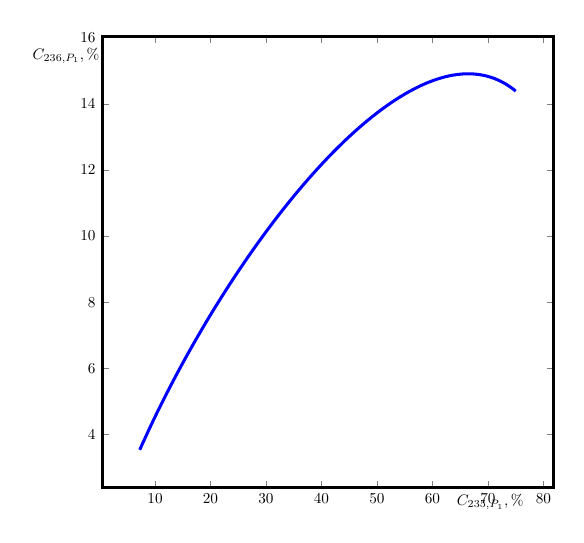
\begin{tikzpicture}[,
scale=0.55]
\begin{axis}[
  xlabel style = {{at={(axis description cs:.86,0)}}},
  ylabel = {$C_{236,P_1}, \%$},
  ylabel style = {{at={(axis description cs:-0.08,.925)},rotate=270,anchor=south}},
  xlabel = {$C_{235,P_1}, \%$},
  width=12cm, height=12cm, line width=2pt
]

\addplot+[
  mark = {none}
] coordinates {
  (7.249999999999999, 3.53615590203731)
  (7.5, 3.6301697421879324)
  (7.75, 3.7233878913807814)
  (9.0, 4.178384420475848)
  (9.25, 4.267311863147327)
  (9.5, 4.355591706436377)
  (9.75, 4.443240216826369)
  (10.0, 4.530272964973655)
  (10.25, 4.6167036807495)
  (10.5, 4.702546874830063)
  (10.75, 4.787815230535367)
  (11.0, 4.872521041434856)
  (11.25, 4.956676062608216)
  (11.5, 5.040291201516588)
  (11.75, 5.123377081328043)
  (12.0, 5.205943733099562)
  (12.25, 5.2880007135300335)
  (12.5, 5.3695571352835545)
  (12.75, 5.450621694782576)
  (13.0, 5.531202697727066)
  (13.25, 5.611308082565347)
  (13.5, 5.690945442116223)
  (13.750000000000002, 5.770122043519018)
  (14.000000000000002, 5.848844846668512)
  (14.249999999999998, 5.927120943517561)
  (14.499999999999998, 6.004955896369638)
  (14.75, 6.0823562516358045)
  (15.0, 6.159327898858619)
  (15.25, 6.235876494180575)
  (15.5, 6.312007472152414)
  (15.75, 6.387726056743825)
  (16.0, 6.463037271621652)
  (16.25, 6.537945949754745)
  (16.5, 6.6124567423989)
  (16.75, 6.686574127509702)
  (17.0, 6.760302417629875)
  (17.25, 6.833645767285421)
  (17.5, 6.906608179932726)
  (17.75, 6.979193460224773)
  (18.0, 7.051405433358855)
  (18.25, 7.123247698790795)
  (18.5, 7.194723597183689)
  (18.75, 7.265836525325857)
  (19.0, 7.3365897047341075)
  (19.25, 7.406986244281054)
  (19.5, 7.477029144634602)
  (19.75, 7.546721302114087)
  (20.0, 7.616065512802825)
  (20.25, 7.6850644760781215)
  (20.5, 7.753720798105427)
  (20.75, 7.822036995123883)
  (21.0, 7.890015496561889)
  (21.25, 7.957658647992906)
  (21.5, 8.024968713941234)
  (21.75, 8.091947880546488)
  (22.0, 8.158598258095118)
  (22.25, 8.224921883426726)
  (22.5, 8.290920722222234)
  (22.75, 8.356596671180586)
  (23.0, 8.421951560090129)
  (23.25, 8.48698715380064)
  (23.5, 8.551705154101137)
  (23.75, 8.616107201508775)
  (24.0, 8.680194876973287)
  (24.25, 8.743969703501543)
  (24.5, 8.807433147706348)
  (24.75, 8.870586621283188)
  (25.0, 8.933431482418722)
  (25.25, 8.99596903713423)
  (25.5, 9.05820054056739)
  (25.75, 9.120127198195172)
  (26.0, 9.181750166055934)
  (26.25, 9.243070555689883)
  (26.5, 9.304089429388243)
  (26.75, 9.364807789311795)
  (27.0, 9.425226645417347)
  (27.250000000000004, 9.485346904322629)
  (27.500000000000004, 9.545169456681242)
  (27.750000000000004, 9.604695146818546)
  (28.000000000000004, 9.66392478497117)
  (28.249999999999996, 9.722859131047011)
  (28.499999999999996, 9.781498912357927)
  (28.749999999999996, 9.839844815532432)
  (28.999999999999996, 9.897897490099387)
  (29.25, 9.955657549587547)
  (29.5, 10.013125563166687)
  (29.75, 10.070302072709467)
  (30.0, 10.127187580081662)
  (30.25, 10.183782553207218)
  (30.5, 10.240087424887575)
  (30.75, 10.29610259368837)
  (31.0, 10.35182842437778)
  (31.25, 10.407265248340995)
  (31.5, 10.462413363971727)
  (31.75, 10.517273037041535)
  (32.0, 10.571844501047499)
  (32.25, 10.626127957538959)
  (32.5, 10.680123576423888)
  (32.75, 10.733831496255458)
  (33.0, 10.787251824499304)
  (33.25, 10.84038463778211)
  (33.5, 10.893229982121671)
  (33.75, 10.945787873139242)
  (34.0, 10.998058296254358)
  (34.25, 11.050041206862428)
  (34.5, 11.101736530495813)
  (34.75, 11.15314416296819)
  (35.0, 11.204263970503044)
  (35.25, 11.25509578984613)
  (35.5, 11.305639428362488)
  (35.75, 11.355894664118043)
  (36.0, 11.405861245946076)
  (36.25, 11.455538893498819)
  (36.5, 11.504927297284242)
  (36.75, 11.554026118688302)
  (37.0, 11.60283498998272)
  (37.25, 11.651353514318432)
  (37.5, 11.69958126570481)
  (37.75, 11.747517788974841)
  (38.0, 11.795162599736175)
  (38.25, 11.842515184308185)
  (38.5, 11.889574999645104)
  (38.75, 11.936341473245244)
  (39.0, 11.982814003046293)
  (39.25, 12.028991957306657)
  (39.5, 12.074874674472918)
  (39.75, 12.1204614630333)
  (40.0, 12.16575160135707)
  (40.25, 12.210744337519946)
  (40.5, 12.25543888911523)
  (40.75, 12.29983444305072)
  (41.0, 12.343930155331297)
  (41.25, 12.38772515082692)
  (41.5, 12.4312185230261)
  (41.75, 12.47440933377441)
  (42.0, 12.517296612998251)
  (42.25, 12.559879358413276)
  (42.5, 12.60215653521756)
  (42.75, 12.644127075769168)
  (43.0, 12.685789879247949)
  (43.25, 12.727143811301259)
  (43.5, 12.768187703673274)
  (43.75, 12.808920353817907)
  (44.0, 12.849340524494576)
  (44.25, 12.889446943346918)
  (44.5, 12.92923830246381)
  (44.75, 12.968713257922552)
  (45.0, 13.007870429313709)
  (45.25, 13.046708399247208)
  (45.5, 13.085225712839415)
  (45.75, 13.123420877180553)
  (46.0, 13.161292360782129)
  (46.25, 13.19883859300391)
  (46.5, 13.236057963459766)
  (46.75, 13.27294882140215)
  (47.0, 13.30950947508424)
  (47.25, 13.345738191099663)
  (47.5, 13.381633193698697)
  (47.75, 13.417192664080702)
  (48.0, 13.452414739661881)
  (48.25, 13.487297513317783)
  (48.5, 13.521839032599758)
  (48.75, 13.556037298924704)
  (49.0, 13.589890266737193)
  (49.25, 13.623395842643216)
  (49.5, 13.65655188451468)
  (49.75, 13.689356200563655)
  (50.0, 13.721806548385887)
  (50.24999999999999, 13.753900633971716)
  (50.5, 13.785636110684187)
  (50.74999999999999, 13.817010578202948)
  (51.0, 13.848021581432835)
  (51.24999999999999, 13.878666609376014)
  (51.5, 13.90894309396646)
  (51.74999999999999, 13.938848408865463)
  (52.0, 13.968379868216896)
  (52.25, 13.997534725360817)
  (52.5, 14.026310171504008)
  (52.75, 14.054703334345897)
  (53.0, 14.082711276658246)
  (53.25, 14.110330994817197)
  (53.5, 14.137559417285539)
  (53.75, 14.164393403043887)
  (54.0, 14.190829739968466)
  (54.25, 14.216865143153898)
  (54.50000000000001, 14.242496253178649)
  (54.75, 14.267719634311272)
  (55.00000000000001, 14.29253177265494)
  (55.25, 14.31692907422818)
  (55.50000000000001, 14.340907862979199)
  (55.75, 14.364464378731313)
  (56.00000000000001, 14.387594775056817)
  (56.25, 14.41029511707643)
  (56.49999999999999, 14.43256137918156)
  (56.75, 14.454389442676034)
  (56.99999999999999, 14.475775093334416)
  (57.25, 14.496714018873359)
  (57.49999999999999, 14.517201806332473)
  (57.75, 14.537233939361164)
  (57.99999999999999, 14.556805795407463)
  (58.25, 14.575912642804829)
  (58.5, 14.594549637752763)
  (58.75, 14.612711821186696)
  (59.0, 14.630394115532585)
  (59.25, 14.647591321341263)
  (59.5, 14.664298113797484)
  (59.75, 14.680509039098242)
  (60.0, 14.696218510694816)
  (60.25, 14.711420805392471)
  (60.5, 14.726110059301774)
  (60.75000000000001, 14.740280263634926)
  (61.0, 14.753925260340218)
  (61.25000000000001, 14.767038737567537)
  (61.5, 14.77961422495724)
  (61.75000000000001, 14.791645088744577)
  (62.0, 14.80312452667113)
  (62.25000000000001, 14.814045562694798)
  (62.5, 14.82440104148875)
  (62.74999999999999, 14.834183622719873)
  (63.0, 14.843385775096499)
  (63.24999999999999, 14.851999770174498)
  (63.5, 14.860017675910678)
  (63.74999999999999, 14.867431349951413)
  (64.0, 14.874232432644053)
  (64.25, 14.880412339757981)
  (64.5, 14.885962254901349)
  (64.75, 14.890873121618975)
  (65.0, 14.895135635155945)
  (65.25, 14.8987402338708)
  (65.5, 14.901677090281165)
  (65.75, 14.903936101723833)
  (66.0, 14.905506880610512)
  (66.25, 14.906378744259074)
  (66.5, 14.906540704279472)
  (66.75, 14.905981455492046)
  (67.0, 14.904689364354997)
  (67.25, 14.90265245687642)
  (67.5, 14.89985840598501)
  (67.75, 14.896294518332201)
  (68.0, 14.891947720497075)
  (68.25, 14.886804544563795)
  (68.5, 14.880851113039755)
  (68.75, 14.874073123081155)
  (69.0, 14.866455829990608)
  (69.25, 14.857984029949975)
  (69.5, 14.848642041949564)
  (69.75, 14.838413688872834)
  (70.0, 14.827282277693895)
  (70.25, 14.815230578742897)
  (70.5, 14.802240803992351)
  (70.75, 14.788294584315132)
  (71.0, 14.773372945662969)
  (71.25, 14.757456284111553)
  (71.5, 14.740524339716659)
  (71.75, 14.72255616912303)
  (72.0, 14.703530116865842)
  (72.25, 14.683423785302397)
  (72.5, 14.662214003109645)
  (72.75, 14.639876792281372)
  (73.0, 14.616387333557304)
  (73.25, 14.591719930215042)
  (73.5, 14.56584797015473)
  (73.75, 14.538743886206158)
  (74.0, 14.510379114587774)
  (74.25, 14.480724051448371)
  (74.5, 14.44974800742369)
  (74.75, 14.417419160143199)
  (75.0, 14.383704504626655)
};

\end{axis}
\end{tikzpicture}


      \caption{{Зависимость $C_{236,P_1}$ от концентрации $^{235}$U в потоке легкой фракции первого каскада ($P_1$){\label{C236P1}}}}
  \end{minipage}
  \end{figure}

\begin{figure}[ht]
    \centering
      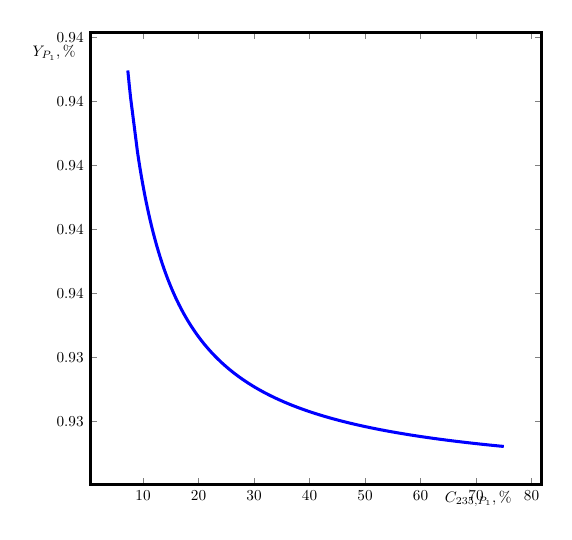
\begin{tikzpicture}[,
scale=0.55]
\begin{axis}[
  xlabel style = {{at={(axis description cs:.86,0)}}},
  ylabel = {$Y_{P_1}, \%$},
  ylabel style = {{at={(axis description cs:-0.08,.925)},rotate=270,anchor=south}},
  xlabel = {$C_{235,P_1}, \%$},
  width=12cm, height=12cm, line width=2pt
]

\addplot+[
  mark = {none}
] coordinates {
  (7.249999999999999, 0.9429735803481439)
  (7.5, 0.9425341685818515)
  (7.75, 0.9421234764346041)
  (9.0, 0.94041610329621)
  (9.25, 0.9401306078742899)
  (9.5, 0.9398602983035926)
  (9.75, 0.9396039943377008)
  (10.0, 0.9393606911865251)
  (10.25, 0.9391292483321038)
  (10.5, 0.9389089989352565)
  (10.75, 0.9386990900391079)
  (11.0, 0.9384988101803494)
  (11.25, 0.9383075317527464)
  (11.5, 0.9381246241854406)
  (11.75, 0.9379495666743339)
  (12.0, 0.9377818644686251)
  (12.25, 0.9376210635377336)
  (12.5, 0.9374667464664416)
  (12.75, 0.9373185288367804)
  (13.0, 0.9371760560306222)
  (13.25, 0.9370390003970017)
  (13.5, 0.936907058736522)
  (13.750000000000002, 0.9367799500622046)
  (14.000000000000002, 0.9366574136019703)
  (14.249999999999998, 0.9365392900740498)
  (14.499999999999998, 0.9364251892833471)
  (14.75, 0.9363149827175828)
  (15.0, 0.936208474358723)
  (15.25, 0.9361054811272185)
  (15.5, 0.9360058318318015)
  (15.75, 0.9359093662199442)
  (16.0, 0.9358159341178939)
  (16.25, 0.9357253946505816)
  (16.5, 0.9356376155328827)
  (16.75, 0.9355524724246426)
  (17.0, 0.9354698483433096)
  (17.25, 0.9353896331273096)
  (17.5, 0.935311722946049)
  (17.75, 0.9352360103170639)
  (18.0, 0.9351624212237206)
  (18.25, 0.9350908701170397)
  (18.5, 0.9350212534666061)
  (18.75, 0.934953503212573)
  (19.0, 0.9348875452932641)
  (19.25, 0.9348233095095012)
  (19.5, 0.934760729295246)
  (19.75, 0.9346997414483528)
  (20.0, 0.9346402859594218)
  (20.25, 0.9345823057927976)
  (20.5, 0.9345257467086877)
  (20.75, 0.9344705570939272)
  (21.0, 0.9344166878048784)
  (21.25, 0.9343640920214809)
  (21.5, 0.9343127251115273)
  (21.75, 0.9342625445043439)
  (22.0, 0.9342135095731237)
  (22.25, 0.9341655815252266)
  (22.5, 0.934118723299827)
  (22.75, 0.9340728994723394)
  (23.0, 0.9340280761651024)
  (23.25, 0.9339842209638533)
  (23.5, 0.9339413028395539)
  (23.75, 0.9338992920751763)
  (24.0, 0.9338581601970827)
  (24.25, 0.9338178799106679)
  (24.5, 0.9337784250399586)
  (24.75, 0.9337397704708864)
  (25.0, 0.9337018920979799)
  (25.25, 0.9336647667742368)
  (25.5, 0.9336283722639531)
  (25.75, 0.9335926871983146)
  (26.0, 0.9335576908889899)
  (26.25, 0.9335233638745569)
  (26.5, 0.9334896869928175)
  (26.75, 0.9334566395417561)
  (27.0, 0.9334242094294047)
  (27.250000000000004, 0.9333923760932793)
  (27.500000000000004, 0.9333611236342547)
  (27.750000000000004, 0.933330436041149)
  (28.000000000000004, 0.9333002988943575)
  (28.249999999999996, 0.933270696773389)
  (28.499999999999996, 0.9332416158004972)
  (28.749999999999996, 0.9332130422925102)
  (28.999999999999996, 0.9331849631797856)
  (29.25, 0.9331573660555152)
  (29.5, 0.933130237814832)
  (29.75, 0.9331035671080765)
  (30.0, 0.9330773423373524)
  (30.25, 0.9330515524716152)
  (30.5, 0.9330261867813012)
  (30.75, 0.9330012348869144)
  (31.0, 0.9329766867448637)
  (31.25, 0.9329525326339856)
  (31.5, 0.9329287631427073)
  (31.75, 0.9329053691568209)
  (32.0, 0.932882341847829)
  (32.25, 0.9328596726618387)
  (32.5, 0.9328373533089653)
  (32.75, 0.9328153757532267)
  (33.0, 0.9327937322028942)
  (33.25, 0.9327724151012848)
  (33.5, 0.932751417117963)
  (33.75, 0.9327307311403369)
  (34.0, 0.9327103502656259)
  (34.25, 0.9326902677931798)
  (34.5, 0.9326704772171357)
  (34.75, 0.9326509722193893)
  (35.0, 0.9326317466628717)
  (35.25, 0.9326127945851099)
  (35.5, 0.9325941101920618)
  (35.75, 0.9325756878522123)
  (36.0, 0.9325575220909124)
  (36.25, 0.9325396075849557)
  (36.5, 0.9325219391573771)
  (36.75, 0.9325045117724672)
  (37.0, 0.932487320530984)
  (37.25, 0.932470360665564)
  (37.5, 0.9324536275363126)
  (37.75, 0.9324371166265735)
  (38.0, 0.9324208235388622)
  (38.25, 0.9324047439909642)
  (38.5, 0.9323888738121793)
  (38.75, 0.9323732089397176)
  (39.0, 0.932357745415231)
  (39.25, 0.9323424793814786)
  (39.5, 0.9323274070791191)
  (39.75, 0.9323125248436243)
  (40.0, 0.9322978291023086)
  (40.25, 0.93228331637147)
  (40.5, 0.9322689832536369)
  (40.75, 0.9322548264349162)
  (41.0, 0.932240842682439)
  (41.25, 0.9322270288418999)
  (41.5, 0.9322133818351835)
  (41.75, 0.9321998986580795)
  (42.0, 0.932186576378077)
  (42.25, 0.9321734121322386)
  (42.5, 0.9321604031251481)
  (42.75, 0.9321475466269334)
  (43.0, 0.932134839971355)
  (43.25, 0.9321222805539644)
  (43.5, 0.9321098658303225)
  (43.75, 0.9320975933142823)
  (44.0, 0.9320854605763292)
  (44.25, 0.9320734652419774)
  (44.5, 0.9320616049902191)
  (44.75, 0.9320498775520307)
  (45.0, 0.9320382807089221)
  (45.25, 0.9320268122915404)
  (45.5, 0.9320154701783148)
  (45.75, 0.9320042522941494)
  (46.0, 0.9319931566091586)
  (46.25, 0.9319821811374395)
  (46.5, 0.9319713239358896)
  (46.75, 0.9319605831030593)
  (47.0, 0.9319499567780422)
  (47.25, 0.9319394431393982)
  (47.5, 0.9319290404041155)
  (47.75, 0.9319187468266008)
  (48.0, 0.9319085606977032)
  (48.25, 0.9318984803437683)
  (48.5, 0.9318885041257213)
  (48.75, 0.931878630438178)
  (49.0, 0.9318688577085854)
  (49.25, 0.9318591843963846)
  (49.5, 0.9318496089922014)
  (49.75, 0.9318401300170464)
  (50.0, 0.9318307460215993)
  (50.24999999999999, 0.9318214555854267)
  (50.5, 0.9318122573162769)
  (50.74999999999999, 0.9318031498493864)
  (51.0, 0.9317941318468042)
  (51.24999999999999, 0.9317852019967362)
  (51.5, 0.9317763590129103)
  (51.74999999999999, 0.9317676016339578)
  (52.0, 0.9317589286228131)
  (52.25, 0.9317503387661327)
  (52.5, 0.931741830873728)
  (52.75, 0.931733403778016)
  (53.0, 0.9317250563334861)
  (53.25, 0.9317167874161782)
  (53.5, 0.9317085959231819)
  (53.75, 0.9317004807721432)
  (54.0, 0.931692440900789)
  (54.25, 0.9316844752664635)
  (54.50000000000001, 0.9316765828456773)
  (54.75, 0.9316687626336685)
  (55.00000000000001, 0.9316610136439782)
  (55.25, 0.9316533349080319)
  (55.50000000000001, 0.9316457254747406)
  (55.75, 0.9316381844101039)
  (56.00000000000001, 0.931630710796831)
  (56.25, 0.9316233037339667)
  (56.49999999999999, 0.9316159623365298)
  (56.75, 0.9316086857351616)
  (56.99999999999999, 0.9316014730757813)
  (57.25, 0.9315943235192528)
  (57.49999999999999, 0.9315872362410585)
  (57.75, 0.931580210430983)
  (57.99999999999999, 0.931573245292804)
  (58.25, 0.9315663400439913)
  (58.5, 0.9315594939154137)
  (58.75, 0.9315527061510542)
  (59.0, 0.9315459760077303)
  (59.25, 0.9315393027548242)
  (59.5, 0.931532685674017)
  (59.75, 0.9315261240590323)
  (60.0, 0.9315196172153832)
  (60.25, 0.9315131644601294)
  (60.5, 0.9315067651216355)
  (60.75000000000001, 0.9315004185393411)
  (61.0, 0.9314941240635298)
  (61.25000000000001, 0.9314878810551117)
  (61.5, 0.9314816888854031)
  (61.75000000000001, 0.9314755469359176)
  (62.0, 0.9314694545981599)
  (62.25000000000001, 0.9314634112734241)
  (62.5, 0.931457416372598)
  (62.74999999999999, 0.9314514693159716)
  (63.0, 0.9314455695330497)
  (63.24999999999999, 0.9314397164623709)
  (63.5, 0.9314339095513262)
  (63.74999999999999, 0.9314281482559894)
  (64.0, 0.9314224320409429)
  (64.25, 0.9314167603791144)
  (64.5, 0.9314111327516149)
  (64.75, 0.9314055486475776)
  (65.0, 0.9314000075640068)
  (65.25, 0.931394509005624)
  (65.5, 0.931389052484721)
  (65.75, 0.9313836375210176)
  (66.0, 0.9313782636415157)
  (66.25, 0.9313729303803665)
  (66.5, 0.9313676372787325)
  (66.75, 0.9313623838846578)
  (67.0, 0.9313571697529365)
  (67.25, 0.9313519944449897)
  (67.5, 0.9313468575287408)
  (67.75, 0.9313417585784945)
  (68.0, 0.9313366971748196)
  (68.25, 0.9313316729044342)
  (68.5, 0.9313266853600918)
  (68.75, 0.9313217341404716)
  (69.0, 0.9313168188500702)
  (69.25, 0.9313119390990958)
  (69.5, 0.931307094503365)
  (69.75, 0.9313022846842016)
  (70.0, 0.9312975092683368)
  (70.25, 0.9312927678878127)
  (70.5, 0.9312880601798873)
  (70.75, 0.9312833857869411)
  (71.0, 0.931278744356386)
  (71.25, 0.931274135540576)
  (71.5, 0.9312695589967197)
  (71.75, 0.9312650143867948)
  (72.0, 0.9312605013774637)
  (72.25, 0.9312560196399905)
  (72.5, 0.931251568850163)
  (72.75, 0.9312471486882106)
  (73.0, 0.9312427588387278)
  (73.25, 0.9312383989905995)
  (73.5, 0.9312340688369235)
  (73.75, 0.9312297680749403)
  (74.0, 0.9312254964059601)
  (74.25, 0.9312212535352923)
  (74.5, 0.9312170391721765)
  (74.75, 0.9312128530297155)
  (75.0, 0.9312086948248076)
};

\end{axis}
\end{tikzpicture}


    \caption{Зависимость степени извлечения $^{235}$U в первом каскаде от концентрации $^{235}$U в потоке легкой фракции первого каскада ($P_1$)}\label{ex1P1}
\end{figure}

\begin{figure}[ht]
    \centering
    \begin{minipage}{.5\textwidth}
        \centering
        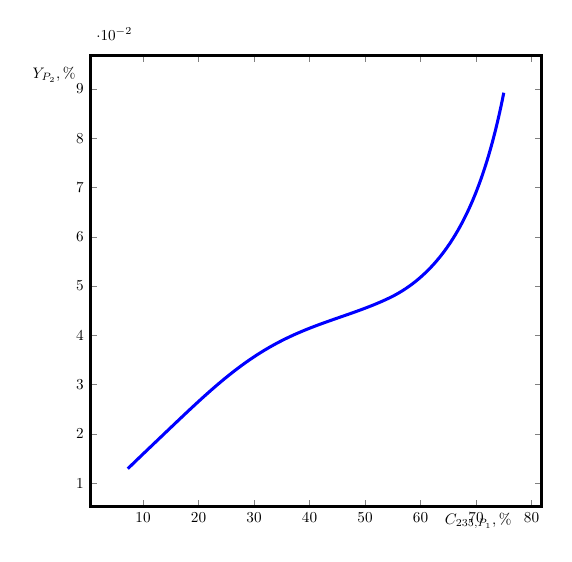
\begin{tikzpicture}[,
scale=0.55]
\begin{axis}[
  xlabel style = {{at={(axis description cs:.86,0)}}},
  ylabel = {$Y_{P_2}, \%$},
  ylabel style = {{at={(axis description cs:-0.08,.925)},rotate=270,anchor=south}},
  xlabel = {$C_{235,P_1}, \%$},
  width=12cm, height=12cm, line width=2pt
]

\addplot+[
  mark = {none}
] coordinates {
  (7.249999999999999, 0.012923554798586022)
  (7.5, 0.013199739119486683)
  (7.75, 0.013474696620546697)
  (9.0, 0.014835844159761566)
  (9.25, 0.01510617585240297)
  (9.5, 0.015376061504723672)
  (9.75, 0.01564559392362786)
  (10.0, 0.015914844246108218)
  (10.25, 0.01618386333970585)
  (10.5, 0.01645270733124181)
  (10.75, 0.016721417238625687)
  (11.0, 0.01699003220133403)
  (11.25, 0.01725857688494721)
  (11.5, 0.017527080310964664)
  (11.75, 0.01779556597777132)
  (12.0, 0.01806405958107595)
  (12.25, 0.018332555093726124)
  (12.5, 0.018601080925494756)
  (12.75, 0.018869585145292415)
  (13.0, 0.01913815302604804)
  (13.25, 0.019406725504658908)
  (13.5, 0.01967532930475323)
  (13.750000000000002, 0.019943890666373254)
  (14.000000000000002, 0.02021246144072858)
  (14.249999999999998, 0.020480997655316285)
  (14.499999999999998, 0.02074949929233362)
  (14.75, 0.02101790673435908)
  (15.0, 0.021286211346583633)
  (15.25, 0.02155439269947379)
  (15.5, 0.021822416522390444)
  (15.75, 0.0220902443564218)
  (16.0, 0.022357864492131247)
  (16.25, 0.022625219403596502)
  (16.5, 0.022892275641345498)
  (16.75, 0.023159014816990616)
  (17.0, 0.023425358304878643)
  (17.25, 0.02369129809690832)
  (17.5, 0.02395677957882435)
  (17.75, 0.02422175532463473)
  (18.0, 0.024486190073562817)
  (18.25, 0.02475003064311657)
  (18.5, 0.025013233289132793)
  (18.75, 0.02527574854954156)
  (19.0, 0.025537521751383505)
  (19.25, 0.0257985176584901)
  (19.5, 0.026058675984437032)
  (19.75, 0.026317952592806608)
  (20.0, 0.026576292183625366)
  (20.25, 0.026833659733272782)
  (20.5, 0.02709000034294488)
  (20.75, 0.02734523686348299)
  (21.0, 0.027599361152286908)
  (21.25, 0.027852294351571723)
  (21.5, 0.028104007883923893)
  (21.75, 0.028354433860149266)
  (22.0, 0.02860353739799309)
  (22.25, 0.028851260014448828)
  (22.5, 0.02909757026673612)
  (22.75, 0.029342411370142946)
  (23.0, 0.029585745691931065)
  (23.25, 0.02982750338538892)
  (23.5, 0.030067665419024777)
  (23.75, 0.030306188851254884)
  (24.0, 0.030543030653819678)
  (24.25, 0.030778116936435798)
  (24.5, 0.03101146998016283)
  (24.75, 0.031242999547830986)
  (25.0, 0.03147270042779003)
  (25.25, 0.03170047947607853)
  (25.5, 0.03192642050516711)
  (25.75, 0.032150342431431514)
  (26.0, 0.03237233278015945)
  (26.25, 0.03259232792293723)
  (26.5, 0.03281026689366049)
  (26.75, 0.03302614116361476)
  (27.0, 0.03323993726065839)
  (27.250000000000004, 0.03345162059966954)
  (27.500000000000004, 0.033661172637723204)
  (27.750000000000004, 0.033868573128106295)
  (28.000000000000004, 0.034073803639499016)
  (28.249999999999996, 0.034276836638280773)
  (28.499999999999996, 0.034477659156021516)
  (28.749999999999996, 0.03467629830792862)
  (28.999999999999996, 0.034872691594575386)
  (29.25, 0.0350668565699536)
  (29.5, 0.035258768675153436)
  (29.75, 0.03544843172154525)
  (30.0, 0.035635820116519085)
  (30.25, 0.03582096465094997)
  (30.5, 0.036003870923382905)
  (30.75, 0.03618449687045527)
  (31.0, 0.03636287163768105)
  (31.25, 0.036538988366208947)
  (31.5, 0.03671285072046419)
  (31.75, 0.0368845011771344)
  (32.0, 0.037053890756417525)
  (32.25, 0.03722108953423341)
  (32.5, 0.03738605977258062)
  (32.75, 0.037548873239688675)
  (33.0, 0.03770948224709088)
  (33.25, 0.03786795104248854)
  (33.5, 0.03802425432982665)
  (33.75, 0.03817847485201748)
  (34.0, 0.03833057696384412)
  (34.25, 0.038480613510783204)
  (34.5, 0.03862859296420825)
  (34.75, 0.03877454809942593)
  (35.0, 0.038918529904836754)
  (35.25, 0.039060519399677585)
  (35.5, 0.03920058963866071)
  (35.75, 0.03933875375080575)
  (36.0, 0.03947504579983738)
  (36.25, 0.03960949540343333)
  (36.5, 0.039742159200397455)
  (36.75, 0.03987305526946869)
  (37.0, 0.04000220623084066)
  (37.25, 0.040129684859721175)
  (37.5, 0.04025549097292606)
  (37.75, 0.04037970356451521)
  (38.0, 0.040502336079678396)
  (38.25, 0.04062343723334888)
  (38.5, 0.0407430559217023)
  (38.75, 0.04086122317649625)
  (39.0, 0.04097800413090023)
  (39.25, 0.041093424867235134)
  (39.5, 0.041207535952668815)
  (39.75, 0.04132039052365175)
  (40.0, 0.041432044505666295)
  (40.25, 0.04154250572035977)
  (40.5, 0.041651858366318885)
  (40.75, 0.041760150258919576)
  (41.0, 0.04186741434766223)
  (41.25, 0.04197371715097869)
  (41.5, 0.04207908945027759)
  (41.75, 0.04218359541943715)
  (42.0, 0.04228727756208433)
  (42.25, 0.04239019977940285)
  (42.5, 0.04249241737817498)
  (42.75, 0.04259394834564992)
  (43.0, 0.04269490031052967)
  (43.25, 0.04279528190276257)
  (43.5, 0.04289516503782189)
  (43.75, 0.04299459223600341)
  (44.0, 0.04309362487968042)
  (44.25, 0.04319232314347877)
  (44.5, 0.04329072680955265)
  (44.75, 0.04338889807314839)
  (45.0, 0.04348689690655575)
  (45.25, 0.04358477217271762)
  (45.5, 0.04368258379790392)
  (45.75, 0.04378037944872461)
  (46.0, 0.04387822208695055)
  (46.25, 0.04397616809005704)
  (46.5, 0.0440742693915369)
  (46.75, 0.04417258631790862)
  (47.0, 0.04427117545478764)
  (47.25, 0.04437009128342893)
  (47.5, 0.04446939152675727)
  (47.75, 0.04456913572776445)
  (48.0, 0.04466938436658935)
  (48.25, 0.04477019347047057)
  (48.5, 0.04487161660712592)
  (48.75, 0.04497371786645341)
  (49.0, 0.045076555595675215)
  (49.25, 0.045180190851415544)
  (49.5, 0.04528468242679774)
  (49.75, 0.04539009068941302)
  (50.0, 0.045496471763642035)
  (50.24999999999999, 0.04560389771370899)
  (50.5, 0.04571242549310311)
  (50.74999999999999, 0.045822115386528785)
  (51.0, 0.04593303432818077)
  (51.24999999999999, 0.0460452437774609)
  (51.5, 0.04615880646127439)
  (51.74999999999999, 0.04627379122708482)
  (52.0, 0.046390263387318394)
  (52.25, 0.0465082888387748)
  (52.5, 0.04662793641020282)
  (52.75, 0.046749273434624955)
  (53.0, 0.04687236927687734)
  (53.25, 0.04699729632302502)
  (53.5, 0.047124124652799276)
  (53.75, 0.04725292864883703)
  (54.0, 0.047383781501358795)
  (54.25, 0.047516640826682825)
  (54.50000000000001, 0.04765165000448252)
  (54.75, 0.04779070772885918)
  (55.00000000000001, 0.04793388407371396)
  (55.25, 0.04808124067452979)
  (55.50000000000001, 0.04823284822051434)
  (55.75, 0.04838877880356654)
  (56.00000000000001, 0.04854910713926176)
  (56.25, 0.0487139107580995)
  (56.49999999999999, 0.04888327011924098)
  (56.75, 0.04905726871939483)
  (56.99999999999999, 0.04923599320555175)
  (57.25, 0.04941953349309538)
  (57.49999999999999, 0.049607982889922284)
  (57.75, 0.04980143822692551)
  (57.99999999999999, 0.04999999999528439)
  (58.25, 0.05020377249086913)
  (58.5, 0.05041286383240578)
  (58.75, 0.050627386724433864)
  (59.0, 0.05084745758736279)
  (59.25, 0.05107319755512561)
  (59.5, 0.051304732403819595)
  (59.75, 0.05154219275284606)
  (60.0, 0.05178571427498955)
  (60.25, 0.052035437916974084)
  (60.5, 0.052291510131729745)
  (60.75000000000001, 0.05255408312334193)
  (61.0, 0.052823315105655355)
  (61.25000000000001, 0.05309937057550799)
  (61.5, 0.053382390391809885)
  (61.75000000000001, 0.05367262357594245)
  (62.0, 0.053970210872459755)
  (62.25000000000001, 0.05427534606643293)
  (62.5, 0.05458823053462359)
  (62.74999999999999, 0.054909073712433615)
  (63.0, 0.055238093564214205)
  (63.24999999999999, 0.05557551706293293)
  (63.5, 0.055921580684515464)
  (63.74999999999999, 0.05627653092148867)
  (64.0, 0.05664062482021029)
  (64.25, 0.057014130545594115)
  (64.5, 0.057397327977183346)
  (64.75, 0.05779050934019511)
  (65.0, 0.05819397987533077)
  (65.25, 0.058608058551005926)
  (65.5, 0.05903307882201348)
  (65.75, 0.05946938943861364)
  (66.0, 0.05991735531041932)
  (66.25, 0.060377358429662596)
  (66.5, 0.06084979885883913)
  (66.75, 0.06133509578805925)
  (67.0, 0.06183368866795101)
  (67.25, 0.06234603842444662)
  (67.5, 0.06287262876238231)
  (67.75, 0.06341396756551021)
  (68.0, 0.06397058840119732)
  (68.25, 0.06454305213901897)
  (68.5, 0.06513194869320686)
  (68.75, 0.06573789890011136)
  (69.0, 0.06636155654281364)
  (69.25, 0.06700361053638136)
  (69.5, 0.06766478728862088)
  (69.75, 0.06834585325277583)
  (70.0, 0.06904761769029853)
  (70.25, 0.06977093566381448)
  (70.5, 0.07051671128248153)
  (70.75, 0.07128590122435516)
  (71.0, 0.07207951856288806)
  (71.25, 0.07289866421817601)
  (71.5, 0.07374443699879087)
  (71.75, 0.07461806444943925)
  (72.0, 0.07552083288790713)
  (72.25, 0.07645411057528477)
  (72.5, 0.07741935431954458)
  (72.75, 0.07841811672870524)
  (73.0, 0.07945205418944855)
  (73.25, 0.08052293565717356)
  (73.5, 0.08163265235550617)
  (73.75, 0.08278322849683495)
  (74.0, 0.08397683315159478)
  (74.25, 0.08521579341240888)
  (74.5, 0.08650260902094255)
  (74.75, 0.08783996865062317)
  (75.0, 0.08923076806799389)
};

\end{axis}
\end{tikzpicture}


  \caption{{Зависимость степени извлечения $^{235}$U в потоке $P_2$ второго каскаде от концентрации $^{235}$U в потоке легкой фракции первого каскада ($P_1$){\label{EX_P2}}}}
  \end{minipage}%
    \begin{minipage}{.5\textwidth}
      \centering
      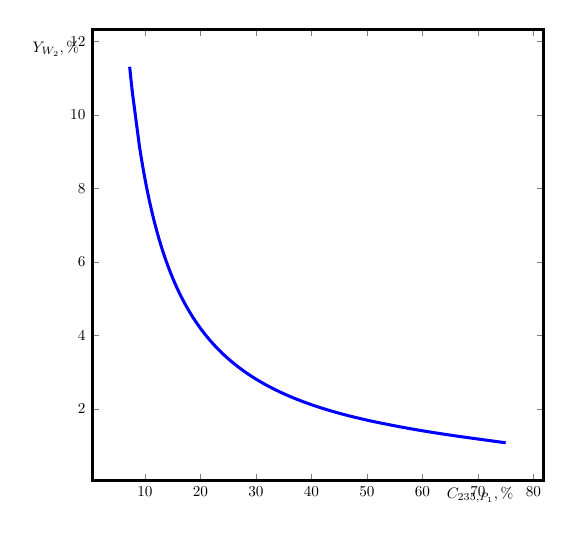
\begin{tikzpicture}[,
scale=0.55]
\begin{axis}[
  xlabel style = {{at={(axis description cs:.86,0)}}},
  ylabel = {$Y_{W_2}, \%$},
  ylabel style = {{at={(axis description cs:-0.08,.925)},rotate=270,anchor=south}},
  xlabel = {$C_{235,P_1}, \%$},
  width=12cm, height=12cm, line width=2pt
]

\addplot+[
  mark = {none}
] coordinates {
  (7.249999999999999, 11.308938082660143)
  (7.5, 10.941238256002066)
  (7.75, 10.596917929073102)
  (9.0, 9.158406041255347)
  (9.25, 8.916705059087402)
  (9.5, 8.68753903861283)
  (9.75, 8.469952785107713)
  (10.0, 8.26308558787556)
  (10.25, 8.06616166185902)
  (10.5, 7.878476181525796)
  (10.75, 7.699391062595429)
  (11.0, 7.5283253963458865)
  (11.25, 7.364749438702721)
  (11.5, 7.208179512844431)
  (11.75, 7.058172487738097)
  (12.0, 6.914321996946741)
  (12.25, 6.776254645379322)
  (12.5, 6.643626656491899)
  (12.75, 6.516121117087158)
  (13.0, 6.393445160618992)
  (13.25, 6.275328029808503)
  (13.5, 6.16151878446214)
  (13.750000000000002, 6.0517847216659355)
  (14.000000000000002, 5.9459094995907495)
  (14.249999999999998, 5.843691593778731)
  (14.499999999999998, 5.744944305210665)
  (14.75, 5.649492522349494)
  (15.0, 5.557173012263817)
  (15.25, 5.467833184750334)
  (15.5, 5.381330242481839)
  (15.75, 5.29753039808877)
  (16.0, 5.216308138079466)
  (16.25, 5.137545673388782)
  (16.5, 5.0611322789585715)
  (16.75, 4.986963778155791)
  (17.0, 4.914942151588445)
  (17.25, 4.844974944099294)
  (17.5, 4.776975002021388)
  (17.75, 4.710860074547931)
  (18.0, 4.64655234339496)
  (18.25, 4.583978302848187)
  (18.5, 4.523068457850149)
  (18.75, 4.463756904076323)
  (19.0, 4.405981222509228)
  (19.25, 4.349682194318292)
  (19.5, 4.294803647580376)
  (19.75, 4.241292219110959)
  (20.0, 4.189097210629755)
  (20.25, 4.138170389226074)
  (20.5, 4.088465883415996)
  (20.75, 4.039940045736645)
  (21.0, 3.992551216105284)
  (21.25, 3.946259763973416)
  (21.5, 3.901027834557081)
  (21.75, 3.8568193484250894)
  (22.0, 3.813599819552377)
  (22.25, 3.771336330008835)
  (22.5, 3.7299973860067372)
  (22.75, 3.689552899163231)
  (23.0, 3.64997406051873)
  (23.25, 3.6112333303816135)
  (23.5, 3.5733042771581878)
  (23.75, 3.5361616027085683)
  (24.0, 3.499781057489339)
  (24.25, 3.4641394221709754)
  (24.5, 3.429214311109948)
  (24.75, 3.3949843648689213)
  (25.0, 3.361428978606563)
  (25.25, 3.3285284585265926)
  (25.5, 3.296263679187779)
  (25.75, 3.2646165515962755)
  (26.0, 3.233569378709585)
  (26.25, 3.2031053007090273)
  (26.5, 3.1732080897106885)
  (26.75, 3.1438620672847897)
  (27.0, 3.1150521221721377)
  (27.250000000000004, 3.086763735562818)
  (27.500000000000004, 3.0589828882700365)
  (27.750000000000004, 3.03169606660359)
  (28.000000000000004, 3.0048902328612006)
  (28.249999999999996, 2.978552821241534)
  (28.499999999999996, 2.9526716864388596)
  (28.749999999999996, 2.927235058598758)
  (28.999999999999996, 2.9022316701490247)
  (29.25, 2.877650548100332)
  (29.5, 2.853481137219079)
  (29.75, 2.829713201452291)
  (30.0, 2.8063368772689348)
  (30.25, 2.783342562688181)
  (30.5, 2.7607209955205554)
  (30.75, 2.738463265389095)
  (31.0, 2.716560669732451)
  (31.25, 2.6950048215211804)
  (31.5, 2.6737875867273244)
  (31.75, 2.6529010428635815)
  (32.0, 2.6323376128350473)
  (32.25, 2.612089823371286)
  (32.5, 2.592150546031968)
  (32.75, 2.5725127495619735)
  (33.0, 2.5531697431828997)
  (33.25, 2.534114914923632)
  (33.5, 2.515341944925078)
  (33.75, 2.49684458226425)
  (34.0, 2.478616885383662)
  (34.25, 2.4606529898192018)
  (34.5, 2.442947246819871)
  (34.75, 2.4254941426018997)
  (35.0, 2.4082882994001156)
  (35.25, 2.391324565413383)
  (35.5, 2.3745978342002445)
  (35.75, 2.358103204094108)
  (36.0, 2.341835885910884)
  (36.25, 2.3257912257534983)
  (36.5, 2.309964666768649)
  (36.75, 2.294351815373658)
  (37.0, 2.2789483907561934)
  (37.25, 2.2637501722255675)
  (37.5, 2.248753127229623)
  (37.75, 2.2339532450212016)
  (38.0, 2.2193466878346597)
  (38.25, 2.20492967987806)
  (38.5, 2.1906985416290055)
  (38.75, 2.1766497058876872)
  (39.0, 2.1627796596322693)
  (39.25, 2.149085018789428)
  (39.5, 2.1355624580812793)
  (39.75, 2.1222087316698284)
  (40.0, 2.1090206703915015)
  (40.25, 2.0959952329123412)
  (40.5, 2.083129372132322)
  (40.75, 2.070420151845564)
  (41.0, 2.057864721740472)
  (41.25, 2.045460264423854)
  (41.5, 2.0332040661481976)
  (41.75, 2.0210934423308666)
  (42.0, 2.009125793378483)
  (42.25, 1.9972985577834614)
  (42.5, 1.985609241745751)
  (42.75, 1.9740554473363596)
  (43.0, 1.9626347385568346)
  (43.25, 1.951344836296281)
  (43.5, 1.940183447767591)
  (43.75, 1.9291483614947245)
  (44.0, 1.9182373957198553)
  (44.25, 1.9074484178931352)
  (44.5, 1.8967793631717316)
  (44.75, 1.8862281887929466)
  (45.0, 1.8757928983674128)
  (45.25, 1.8654715498251901)
  (45.5, 1.8552622313434086)
  (45.75, 1.8451630842818516)
  (46.0, 1.8351722736841225)
  (46.25, 1.8252880097775466)
  (46.5, 1.8155085447206911)
  (46.75, 1.8058321584177248)
  (47.0, 1.7962571700358987)
  (47.25, 1.7867819353826688)
  (47.5, 1.77740484052257)
  (47.75, 1.768124302371785)
  (48.0, 1.7589387687620595)
  (48.25, 1.7498467231312675)
  (48.5, 1.7408466816777866)
  (48.75, 1.7319371793383977)
  (49.0, 1.7231167856618355)
  (49.25, 1.7143840954538763)
  (49.5, 1.7057377331483587)
  (49.75, 1.6971763482141842)
  (50.0, 1.6886986204165686)
  (50.24999999999999, 1.6803032386527652)
  (50.5, 1.6719889319165973)
  (50.74999999999999, 1.6637544499299683)
  (51.0, 1.6555985592022544)
  (51.24999999999999, 1.6475200547746438)
  (51.5, 1.639517752821244)
  (51.74999999999999, 1.6315904852028598)
  (52.0, 1.6237371087380177)
  (52.25, 1.6159565005212448)
  (52.5, 1.608247555060896)
  (52.75, 1.6006091882859579)
  (53.0, 1.5930403335164671)
  (53.25, 1.5855399400203214)
  (53.5, 1.5781069779612882)
  (53.75, 1.5707404313017628)
  (54.0, 1.5634393029421583)
  (54.25, 1.5561699947266738)
  (54.50000000000001, 1.5486786252237992)
  (54.75, 1.541250385657518)
  (55.00000000000001, 1.5338842974768188)
  (55.25, 1.5265793927644467)
  (55.50000000000001, 1.5193347193368578)
  (55.75, 1.512149337785868)
  (56.00000000000001, 1.5050223214319067)
  (56.25, 1.4979527559091468)
  (56.49999999999999, 1.4909397387313017)
  (56.75, 1.4839823788589355)
  (56.99999999999999, 1.477079796269563)
  (57.25, 1.470231121530337)
  (57.49999999999999, 1.4634354953727005)
  (57.75, 1.4566920682684843)
  (57.99999999999999, 1.4500000000067603)
  (58.25, 1.443358459270961)
  (58.5, 1.4367666232749619)
  (58.75, 1.430223677072166)
  (59.0, 1.423728813584936)
  (59.25, 1.417281232819809)
  (59.5, 1.4108801415455623)
  (59.75, 1.4045247528559985)
  (60.0, 1.3982142857284334)
  (60.25, 1.3919479645768518)
  (60.5, 1.3857250187986476)
  (60.75000000000001, 1.3795446823139832)
  (61.0, 1.3734061930967374)
  (61.25000000000001, 1.3673087926959206)
  (61.5, 1.3612517448792396)
  (61.75000000000001, 1.3552342520413951)
  (62.0, 1.3492555912608042)
  (62.25000000000001, 1.3433150127554832)
  (62.5, 1.3374117679043638)
  (62.74999999999999, 1.3315451086476926)
  (63.0, 1.3257142868758063)
  (63.24999999999999, 1.3199185538035)
  (63.5, 1.3141571593269943)
  (63.74999999999999, 1.3084293513606067)
  (64.0, 1.3027343751500857)
  (64.25, 1.2970714725596126)
  (64.5, 1.291439881329227)
  (64.75, 1.2858388342995273)
  (65.0, 1.280267558600114)
  (65.25, 1.2747252747983393)
  (65.5, 1.2692111960044303)
  (65.75, 1.2637245269290585)
  (66.0, 1.258264462888985)
  (66.25, 1.2528301887561804)
  (66.5, 1.2474208778453695)
  (66.75, 1.2420356907346244)
  (67.0, 1.2366737740130802)
  (67.25, 1.2313342589493848)
  (67.5, 1.2260162600738524)
  (67.75, 1.220718873666662)
  (68.0, 1.2154411761437351)
  (68.25, 1.2101822223309906)
  (68.5, 1.2049410436169572)
  (68.75, 1.1997166459724709)
  (69.0, 1.1945080078252341)
  (69.25, 1.1893140777756641)
  (69.5, 1.1841337721390524)
  (69.75, 1.1789659722974732)
  (70.0, 1.173809521843209)
  (70.25, 1.168663223493386)
  (70.5, 1.163525835753493)
  (70.75, 1.1583960693049276)
  (71.0, 1.1532725830892354)
  (71.25, 1.1481539674450998)
  (71.5, 1.1430387798738213)
  (71.75, 1.137925489652258)
  (72.0, 1.1328125005457672)
  (72.25, 1.1276981386659033)
  (72.5, 1.12258064579289)
  (72.75, 1.1174581720500207)
  (73.0, 1.1123287678540947)
  (73.25, 1.107190375055874)
  (73.5, 1.1020408171724956)
  (73.75, 1.0968777886002414)
  (74.0, 1.0916988426799137)
  (74.25, 1.086501378468659)
  (74.5, 1.0812826260503714)
  (74.75, 1.0760396301914672)
  (75.0, 1.0707692321192377)
};

\end{axis}
\end{tikzpicture}


\caption{{Зависимость степени извлечения $^{235}$U в потоке $W_2$ второго каскаде от концентрации $^{235}$U в потоке легкой фракции первого каскада ($P_1$){\label{EX_W2}}}}
    \end{minipage}
\end{figure}

\begin{figure}[ht]
  \centering
  \begin{minipage}{.5\textwidth}
    \centering
    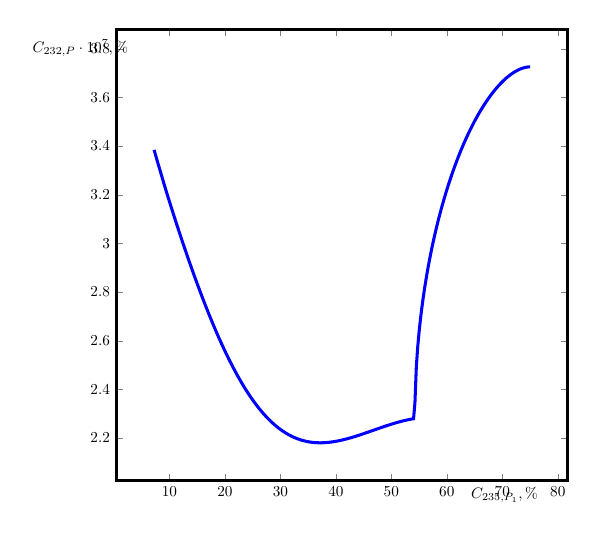
\begin{tikzpicture}[,
scale=0.55]
\begin{axis}[
  xlabel style = {{at={(axis description cs:.86,0)}}},
  ylabel = {$C_{232,P}\cdot10^{7}, \%$},
  ylabel style = {{at={(axis description cs:-0.08,.925)},rotate=270,anchor=south}},
  xlabel = {$C_{235,P_1}, \%$},
  width=12cm, height=12cm, line width=2pt
]

\addplot+[
  mark = {none}
] coordinates {
  (7.249999999999999, 3.3842143149687756)
  (7.5, 3.3639899573365524)
  (7.75, 3.344003772337697)
  (9.0, 3.247180923885222)
  (9.25, 3.2283583724439695)
  (9.5, 3.2097020853414535)
  (9.75, 3.191202973279396)
  (10.0, 3.17285512410164)
  (10.25, 3.154655265568489)
  (10.5, 3.1365990502878103)
  (10.75, 3.118684113526867)
  (11.0, 3.1009076710041024)
  (11.25, 3.083268879211135)
  (11.5, 3.0657662375374883)
  (11.75, 3.0483984751533457)
  (12.0, 3.0311640152203023)
  (12.25, 3.0140649579350716)
  (12.5, 2.9970988176622604)
  (12.75, 2.980272935742599)
  (13.0, 2.963577421448504)
  (13.25, 2.9470200944989005)
  (13.5, 2.9305978334382417)
  (13.750000000000002, 2.9143197228196684)
  (14.000000000000002, 2.8981793060375254)
  (14.249999999999998, 2.882181356003909)
  (14.499999999999998, 2.866325480685528)
  (14.75, 2.8506181573018714)
  (15.0, 2.835059096037781)
  (15.25, 2.819649668822359)
  (15.5, 2.804392572431263)
  (15.75, 2.7892907514270564)
  (16.0, 2.7743438986308093)
  (16.25, 2.7595568753542876)
  (16.5, 2.7449313125155674)
  (16.75, 2.730467295160821)
  (17.0, 2.71617156879616)
  (17.25, 2.702042168221155)
  (17.5, 2.6880830609277995)
  (17.75, 2.6742963795296397)
  (18.0, 2.660683588493613)
  (18.25, 2.6472473301438866)
  (18.5, 2.6339894011328364)
  (18.75, 2.6209119629616837)
  (19.0, 2.6080178648266084)
  (19.25, 2.595307290175821)
  (19.5, 2.582783274560423)
  (19.75, 2.5704470398841184)
  (20.0, 2.558300750931584)
  (20.25, 2.5463445889199177)
  (20.5, 2.5345804678012676)
  (20.75, 2.523012466539271)
  (21.0, 2.511638061682186)
  (21.25, 2.500461018571076)
  (21.5, 2.4894806919227044)
  (21.75, 2.478699745531179)
  (22.0, 2.4681180764791675)
  (22.25, 2.457737416673902)
  (22.5, 2.4475571435618892)
  (22.75, 2.4375786435230093)
  (23.0, 2.427802085333702)
  (23.25, 2.418229736733599)
  (23.5, 2.4088603928416)
  (23.75, 2.399693662057542)
  (24.0, 2.3907302242826147)
  (24.25, 2.381972712974044)
  (24.5, 2.3734159660270584)
  (24.75, 2.365064300315776)
  (25.0, 2.3569147442720215)
  (25.25, 2.348971784149393)
  (25.5, 2.3412251002651767)
  (25.75, 2.3336865886358957)
  (26.0, 2.326345860565808)
  (26.25, 2.319204713981513)
  (26.5, 2.312265330107818)
  (26.75, 2.305525285922927)
  (27.0, 2.2989826658034223)
  (27.250000000000004, 2.2926373971109726)
  (27.500000000000004, 2.2864878949303673)
  (27.750000000000004, 2.2805333663310567)
  (28.000000000000004, 2.2747722124196237)
  (28.249999999999996, 2.2692039952602983)
  (28.499999999999996, 2.26382713092149)
  (28.749999999999996, 2.258636830183319)
  (28.999999999999996, 2.2536358651418267)
  (29.25, 2.248820188885055)
  (29.5, 2.244189531831472)
  (29.75, 2.239741376610604)
  (30.0, 2.2354754897487745)
  (30.25, 2.231387153043769)
  (30.5, 2.2274741599614125)
  (30.75, 2.2237378783214305)
  (31.0, 2.2201741100056176)
  (31.25, 2.216781628747637)
  (31.5, 2.2135584400395367)
  (31.75, 2.2104996598025215)
  (32.0, 2.2076075025051827)
  (32.25, 2.204875274794084)
  (32.5, 2.2023042810535007)
  (32.75, 2.199887746150818)
  (33.0, 2.197628384587492)
  (33.25, 2.195519861890813)
  (33.5, 2.1935632423102516)
  (33.75, 2.1917511968164898)
  (34.0, 2.190085496134909)
  (34.25, 2.1885614524021793)
  (34.5, 2.1871773270025434)
  (34.75, 2.1859305818368107)
  (35.0, 2.184816025127349)
  (35.25, 2.183834987231016)
  (35.5, 2.182981731733877)
  (35.75, 2.182254518977843)
  (36.0, 2.1816505796739127)
  (36.25, 2.181167259795179)
  (36.5, 2.180800703801268)
  (36.75, 2.1805488455977655)
  (37.0, 2.180410122639158)
  (37.25, 2.1803792705066956)
  (37.5, 2.180456122147009)
  (37.75, 2.180634886996319)
  (38.0, 2.180915016260582)
  (38.25, 2.1812928547635115)
  (38.5, 2.1817654738955725)
  (38.75, 2.18233043375212)
  (39.0, 2.182983446907331)
  (39.25, 2.1837230526838165)
  (39.5, 2.18454616306163)
  (39.75, 2.1854492159216523)
  (40.0, 2.186428525140957)
  (40.25, 2.187484163651412)
  (40.5, 2.188610916432595)
  (40.75, 2.1898057234698407)
  (41.0, 2.1910670884817818)
  (41.25, 2.1923905098397354)
  (41.5, 2.1937747339259066)
  (41.75, 2.19521613423141)
  (42.0, 2.196712310980311)
  (42.25, 2.1982595281177026)
  (42.5, 2.199854817917085)
  (42.75, 2.2014976582289787)
  (43.0, 2.2031813612342637)
  (43.25, 2.204906303027762)
  (43.5, 2.2066683617202996)
  (43.75, 2.208465370972621)
  (44.0, 2.2102942804514933)
  (44.25, 2.2121517391168566)
  (44.5, 2.2140361767121224)
  (44.75, 2.2159443517401582)
  (45.0, 2.2178726975349194)
  (45.25, 2.2198196973206814)
  (45.5, 2.2217819082766352)
  (45.75, 2.2237571923588817)
  (46.0, 2.22574252418807)
  (46.25, 2.227735178300996)
  (46.5, 2.229732917779297)
  (46.75, 2.2317325884945776)
  (47.0, 2.2337319904462767)
  (47.25, 2.2357282231899474)
  (47.5, 2.237719137372041)
  (47.75, 2.2397017790335614)
  (48.0, 2.2416734463563244)
  (48.25, 2.243631724444802)
  (48.5, 2.245574778711914)
  (48.75, 2.2474990198374534)
  (49.0, 2.2494027538634)
  (49.25, 2.251282705127118)
  (49.5, 2.2531371505768636)
  (49.75, 2.2549628732281177)
  (50.0, 2.2567585572336357)
  (50.24999999999999, 2.258520358044613)
  (50.5, 2.260246169430438)
  (50.74999999999999, 2.2619339633631697)
  (51.0, 2.2635808951696132)
  (51.24999999999999, 2.2651848520498143)
  (51.5, 2.2667431689974036)
  (51.74999999999999, 2.2682533238456375)
  (52.0, 2.2697130825583063)
  (52.25, 2.2711197700592183)
  (52.5, 2.272470996617753)
  (52.75, 2.2737642974319376)
  (53.0, 2.2749972192466688)
  (53.25, 2.2761673260093875)
  (53.5, 2.277272048247744)
  (53.75, 2.278308978259457)
  (54.0, 2.279275388025011)
  (54.25, 2.3452979281112465)
  (54.50000000000001, 2.4935024641759282)
  (54.75, 2.5743328844335798)
  (55.00000000000001, 2.6370005062275355)
  (55.25, 2.6899237615878335)
  (55.50000000000001, 2.73649670931843)
  (55.75, 2.778493430638717)
  (56.00000000000001, 2.8169798337428706)
  (56.25, 2.852655789576913)
  (56.49999999999999, 2.8860101992843674)
  (56.75, 2.91740061188421)
  (56.99999999999999, 2.9470979275560194)
  (57.25, 2.975313253542268)
  (57.49999999999999, 3.00221491780103)
  (57.75, 3.027939719534641)
  (57.99999999999999, 3.0526006367003897)
  (58.25, 3.076292265571921)
  (58.5, 3.0990947698298843)
  (58.75, 3.12107674110136)
  (59.0, 3.1422974867994817)
  (59.25, 3.162808642196739)
  (59.5, 3.182655504709978)
  (59.75, 3.201878067575165)
  (60.0, 3.22051184500215)
  (60.25, 3.23858853795207)
  (60.5, 3.256136576557642)
  (60.75000000000001, 3.273181565968262)
  (61.0, 3.289746655787327)
  (61.25000000000001, 3.3058528484710243)
  (61.5, 3.321521140866596)
  (61.75000000000001, 3.3367645261367422)
  (62.0, 3.3516017767512962)
  (62.25000000000001, 3.3660474552425708)
  (62.5, 3.380114962499678)
  (62.74999999999999, 3.393816649061101)
  (63.0, 3.4071639125574142)
  (63.24999999999999, 3.420167283239585)
  (63.5, 3.43283649921508)
  (63.74999999999999, 3.4451805727637033)
  (64.0, 3.457207848891476)
  (64.25, 3.468926057108763)
  (64.5, 3.480342357269395)
  (64.75, 3.491463380189329)
  (65.0, 3.5022952636548146)
  (65.25, 3.512843684349819)
  (65.5, 3.523113886150587)
  (65.75, 3.5331107051792814)
  (66.0, 3.542838591950143)
  (66.25, 3.552301630897615)
  (66.5, 3.561503557533944)
  (66.75, 3.570447773451082)
  (67.0, 3.5791373593496614)
  (67.25, 3.587575086252096)
  (67.5, 3.595763425033083)
  (67.75, 3.603704554379354)
  (68.0, 3.6114003672737196)
  (68.25, 3.618852476078032)
  (68.5, 3.626062216279264)
  (68.75, 3.633030648943375)
  (69.0, 3.639758561913507)
  (69.25, 3.6462464697740944)
  (69.5, 3.6524946125925744)
  (69.75, 3.65850295343902)
  (70.0, 3.664271174675937)
  (70.25, 3.6697986729995975)
  (70.5, 3.6750845532077956)
  (70.75, 3.680127620660736)
  (71.0, 3.6849263723985906)
  (71.25, 3.6894776257893036)
  (71.5, 3.6937813696691904)
  (71.75, 3.6978341181091987)
  (72.0, 3.7016329515875293)
  (72.25, 3.705174557787524)
  (72.5, 3.7084552089754164)
  (72.75, 3.71147073655744)
  (73.0, 3.7142165025134712)
  (73.25, 3.716687367362542)
  (73.5, 3.7188776542604733)
  (73.75, 3.7207811087737004)
  (74.0, 3.722390853799302)
  (74.25, 3.72369933902449)
  (74.5, 3.7246982842218457)
  (74.75, 3.72537861556757)
  (75.0, 3.7257303940416433)
};

\end{axis}
\end{tikzpicture}


    \caption{{Зависимость концентрации $^{232}$U в потоке НОУ-продукта от концентрации $^{235}$U в потоке легкой фракции первого каскада ($P_1$){\label{C232P}}}}
  \end{minipage}%
  \begin{minipage}{.5\textwidth}
    \centering
    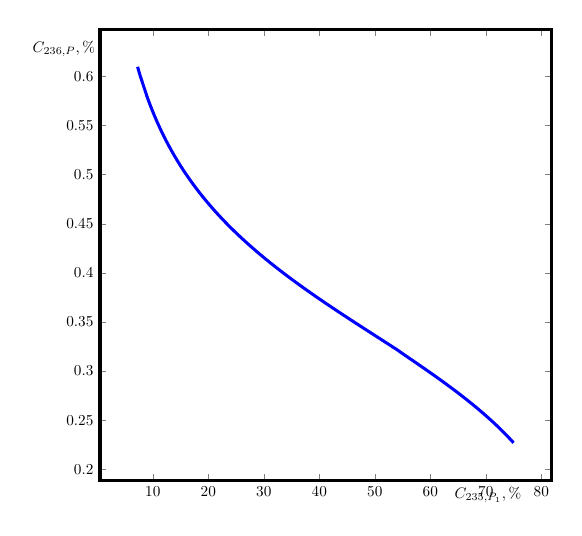
\begin{tikzpicture}[,
scale=0.55]
\begin{axis}[
  xlabel style = {{at={(axis description cs:.86,0)}}},
  ylabel = {$C_{236,P}, \%$},
  ylabel style = {{at={(axis description cs:-0.08,.925)},rotate=270,anchor=south}},
  xlabel = {$C_{235,P_1}, \%$},
  width=12cm, height=12cm, line width=2pt
]

\addplot+[
  mark = {none}
] coordinates {
  (7.249999999999999, 0.6097399654743381)
  (7.5, 0.6047740456261047)
  (7.75, 0.6000029443445043)
  (9.0, 0.5786117582692765)
  (9.25, 0.5747519385847688)
  (9.5, 0.5710112736012622)
  (9.75, 0.567382580245827)
  (10.0, 0.5638593200624819)
  (10.25, 0.5604353551746617)
  (10.5, 0.5571052618016823)
  (10.75, 0.5538638924427196)
  (11.0, 0.5507065332180445)
  (11.25, 0.5476288359845256)
  (11.5, 0.5446267363368124)
  (11.75, 0.5416964939698846)
  (12.0, 0.5388346194465328)
  (12.25, 0.5360378647233518)
  (12.5, 0.5333031967640867)
  (12.75, 0.5306277878675902)
  (13.0, 0.5280089815365097)
  (13.25, 0.5254442997425521)
  (13.5, 0.5229314111496547)
  (13.750000000000002, 0.5204681334363825)
  (14.000000000000002, 0.518052404568894)
  (14.249999999999998, 0.515682335851156)
  (14.499999999999998, 0.5133560098165689)
  (14.75, 0.5110717521001259)
  (15.0, 0.5088279348908167)
  (15.25, 0.5066230195990685)
  (15.5, 0.5044555510075279)
  (15.75, 0.5023241507881899)
  (16.0, 0.5002275098975908)
  (16.25, 0.4981643893161296)
  (16.5, 0.49613361046303395)
  (16.75, 0.49413405159015494)
  (17.0, 0.4921646498930325)
  (17.25, 0.490224388466133)
  (17.5, 0.4883123013199906)
  (17.75, 0.48642746227074474)
  (18.0, 0.4845690004952133)
  (18.25, 0.48273607779965555)
  (18.5, 0.48092788079485027)
  (18.75, 0.47914364773632995)
  (19.0, 0.47738264505585426)
  (19.25, 0.475644169263567)
  (19.5, 0.4739275481362575)
  (19.75, 0.47223213615338294)
  (20.0, 0.47055731510841436)
  (20.25, 0.46890249017092556)
  (20.5, 0.46726709179169457)
  (20.75, 0.4656505745013966)
  (21.0, 0.46405240872911485)
  (21.25, 0.4624720907824638)
  (21.5, 0.4609091320267056)
  (21.75, 0.45936306526522763)
  (22.0, 0.4578334378671866)
  (22.25, 0.45631981567438695)
  (22.5, 0.4548217780328698)
  (22.75, 0.4533389213399613)
  (23.0, 0.45187085443161806)
  (23.25, 0.4504172026336811)
  (23.5, 0.44897759966167505)
  (23.75, 0.44755169420134033)
  (24.0, 0.4461391461082798)
  (24.25, 0.44473962929815547)
  (24.5, 0.44335282071913684)
  (24.75, 0.4419784164410967)
  (25.0, 0.4406161158105224)
  (25.25, 0.43926563438984956)
  (25.5, 0.43792668305791155)
  (25.75, 0.4365990017939596)
  (26.0, 0.4352823179643549)
  (26.25, 0.43397637903082964)
  (26.5, 0.4326809392484011)
  (26.75, 0.43139575529290736)
  (27.0, 0.43012059483599635)
  (27.250000000000004, 0.4288552296530662)
  (27.500000000000004, 0.42759943875472506)
  (27.750000000000004, 0.42635300676890364)
  (28.000000000000004, 0.4251157250587669)
  (28.249999999999996, 0.4238873904571186)
  (28.499999999999996, 0.422667804668709)
  (28.749999999999996, 0.4214567715683885)
  (28.999999999999996, 0.4202541067384582)
  (29.25, 0.41905962501416344)
  (29.5, 0.4178731483801072)
  (29.75, 0.4166945018550688)
  (30.0, 0.41552351681396205)
  (30.25, 0.41436002477022604)
  (30.5, 0.4132038628589284)
  (30.75, 0.41205487582126427)
  (31.0, 0.4109129068842996)
  (31.25, 0.40977780553318455)
  (31.5, 0.4086494239772749)
  (31.75, 0.40752761490047357)
  (32.0, 0.40641224104960444)
  (32.25, 0.40530315935125305)
  (32.5, 0.4042002380013951)
  (32.75, 0.4031033398624612)
  (33.0, 0.4020123392359218)
  (33.25, 0.4009271053030834)
  (33.5, 0.3998475161075762)
  (33.75, 0.3987734444924482)
  (34.0, 0.3977047744009962)
  (34.25, 0.39664138554114503)
  (34.5, 0.3955831634994329)
  (34.75, 0.39452999360808777)
  (35.0, 0.39348176300069715)
  (35.25, 0.3924383650880949)
  (35.5, 0.39139968876717063)
  (35.75, 0.39036562961988)
  (36.0, 0.38933608323323166)
  (36.25, 0.38831094752315964)
  (36.5, 0.3872901196610452)
  (36.75, 0.3862735021150305)
  (37.0, 0.3852609980698089)
  (37.25, 0.38425250872960953)
  (37.5, 0.3832479423049297)
  (37.75, 0.38224720269644463)
  (38.0, 0.3812501996430709)
  (38.25, 0.38025684215722577)
  (38.5, 0.3792670400564057)
  (38.75, 0.37828070636041755)
  (39.0, 0.37729775246288033)
  (39.25, 0.37631809377616643)
  (39.5, 0.37534164504472356)
  (39.75, 0.374368322201958)
  (40.0, 0.3733980420408954)
  (40.25, 0.37243072559859697)
  (40.5, 0.371466289381799)
  (40.75, 0.3705046538252233)
  (41.0, 0.3695457409852989)
  (41.25, 0.36858947193967856)
  (41.5, 0.3676357706381322)
  (41.75, 0.36668455952996865)
  (42.0, 0.3657357636551186)
  (42.25, 0.3647893072049344)
  (42.5, 0.36384511561657995)
  (42.75, 0.3629031178103015)
  (43.0, 0.3619632370179255)
  (43.25, 0.36102540399538097)
  (43.5, 0.3600895457510767)
  (43.75, 0.3591555920448302)
  (44.0, 0.35822347156591133)
  (44.25, 0.3572931139530689)
  (44.5, 0.3563644505122162)
  (44.75, 0.35543741158251324)
  (45.0, 0.35451192852088237)
  (45.25, 0.3535879329003884)
  (45.5, 0.3526653568718215)
  (45.75, 0.3517441334774811)
  (46.0, 0.350824194949608)
  (46.25, 0.34990547445539805)
  (46.5, 0.3489879056538487)
  (46.75, 0.3480714222062852)
  (47.0, 0.3471559577612002)
  (47.25, 0.3462414470469255)
  (47.5, 0.34532782402972223)
  (47.75, 0.3444150233122963)
  (48.0, 0.3435029793749321)
  (48.25, 0.34259162718541347)
  (48.5, 0.341680901691052)
  (48.75, 0.3407707380880676)
  (49.0, 0.3398610708510966)
  (49.25, 0.33895183548242347)
  (49.5, 0.33804296656197724)
  (49.75, 0.33713439972474585)
  (50.0, 0.33622606959092566)
  (50.24999999999999, 0.33531791088336454)
  (50.5, 0.33440985872576046)
  (50.74999999999999, 0.3335018477138046)
  (51.0, 0.3325938122238642)
  (51.24999999999999, 0.3316856866008873)
  (51.5, 0.3307774053656066)
  (51.74999999999999, 0.32986890203219515)
  (52.0, 0.32896011013912924)
  (52.25, 0.32805096332587536)
  (52.5, 0.32714139442495943)
  (52.75, 0.32623133627317114)
  (53.0, 0.3253207211876668)
  (53.25, 0.3244094808175856)
  (53.5, 0.32349754689016924)
  (53.75, 0.32258485013955157)
  (54.0, 0.32167132134952103)
  (54.25, 0.32070153033692234)
  (54.50000000000001, 0.31965581717128416)
  (54.75, 0.3186649856643962)
  (55.00000000000001, 0.3176876938407784)
  (55.25, 0.3167168301830889)
  (55.50000000000001, 0.31574948769083344)
  (55.75, 0.3147841122651859)
  (56.00000000000001, 0.3138197396334534)
  (56.25, 0.312855709368843)
  (56.49999999999999, 0.3118915353988246)
  (56.75, 0.3109268395673056)
  (56.99999999999999, 0.3099613143474313)
  (57.25, 0.30899470044149663)
  (57.49999999999999, 0.30802677258271544)
  (57.75, 0.3070573301347171)
  (57.99999999999999, 0.30608619063728887)
  (58.25, 0.30511318523571407)
  (58.5, 0.30413815536131183)
  (58.75, 0.3031609502298661)
  (59.0, 0.3021814249982214)
  (59.25, 0.30119943926844955)
  (59.5, 0.300214855940926)
  (59.75, 0.299227540283732)
  (60.0, 0.29823735917158745)
  (60.25, 0.29724418045330575)
  (60.5, 0.29624787241768286)
  (60.75000000000001, 0.29524830333542607)
  (61.0, 0.29424534106021194)
  (61.25000000000001, 0.29323885267592165)
  (61.5, 0.2922287061920948)
  (61.75000000000001, 0.29121476152275666)
  (62.0, 0.2901968845627257)
  (62.25000000000001, 0.28917493634094893)
  (62.5, 0.2881487757759231)
  (62.74999999999999, 0.28711825944535735)
  (63.0, 0.2860832413632137)
  (63.24999999999999, 0.285043572761696)
  (63.5, 0.28399910187605615)
  (63.74999999999999, 0.28294967373036917)
  (64.0, 0.2818951299226104)
  (64.25, 0.2808353084075515)
  (64.5, 0.27977004327608646)
  (64.75, 0.2786991645297244)
  (65.0, 0.2776224978490175)
  (65.25, 0.2765398643547751)
  (65.5, 0.2754510803609033)
  (65.75, 0.2743559571177479)
  (66.0, 0.27325430054479755)
  (66.25, 0.27214591095158897)
  (66.5, 0.2710305827456155)
  (66.75, 0.26990810412600813)
  (67.0, 0.26877825676168293)
  (67.25, 0.2676408154525905)
  (67.5, 0.2664955477726123)
  (67.75, 0.2653422136925487)
  (68.0, 0.26418056518154703)
  (68.25, 0.2630103457851618)
  (68.5, 0.2618312901781362)
  (68.75, 0.2606431236897933)
  (69.0, 0.2594455617997734)
  (69.25, 0.2582383096016442)
  (69.5, 0.2570210612316847)
  (69.75, 0.2557934992598948)
  (70.0, 0.2545552940400131)
  (70.25, 0.2533061030150069)
  (70.5, 0.25204556997416416)
  (70.75, 0.2507733242575324)
  (71.0, 0.24948897990304206)
  (71.25, 0.24819213307073193)
  (71.5, 0.2468823665077257)
  (71.75, 0.24555924153979503)
  (72.0, 0.2442223009151359)
  (72.25, 0.24287106668665032)
  (72.5, 0.24150503886633642)
  (72.75, 0.24012369396743663)
  (73.0, 0.23872648342250896)
  (73.25, 0.23731283186410324)
  (73.5, 0.23588213525296062)
  (73.75, 0.2344337588366931)
  (74.0, 0.23296703491954368)
  (74.25, 0.2314812604211779)
  (74.5, 0.2299756941993112)
  (74.75, 0.22844955410733717)
  (75.0, 0.2269020137538657)
};

\end{axis}
\end{tikzpicture}


    \caption{{Зависимость концентрации $^{236}$U в потоке НОУ-продукта от концентрации $^{235}$U в потоке легкой фракции первого каскада ($P_1$){\label{C236P}}}}
\end{minipage}
\end{figure}

\begin{figure}[ht]
    \centering
      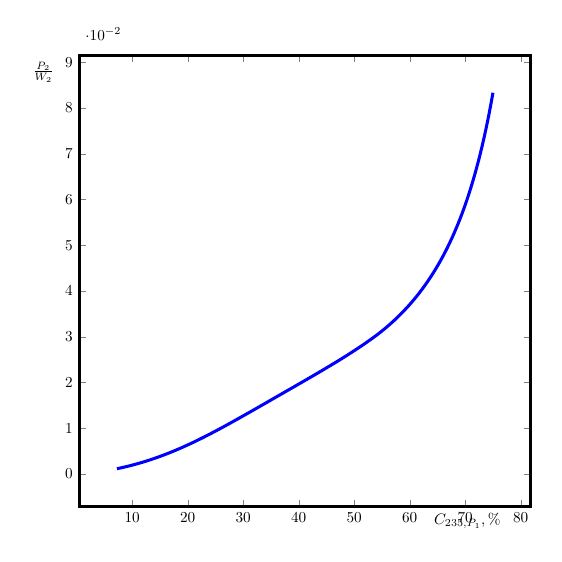
\begin{tikzpicture}[,
scale=0.55]
\begin{axis}[
  xlabel style = {{at={(axis description cs:.86,0)}}},
  ylabel = {$\frac{P_2}{W_2}$},
  ylabel style = {{at={(axis description cs:-0.08,.925)},rotate=270,anchor=south}},
  xlabel = {$C_{235,P_1}, \%$},
  width=12cm, height=12cm, line width=2pt
]

\addplot+[
  mark = {none}
] coordinates {
  (7.249999999999999, 0.0011427735039421208)
  (7.5, 0.0012064209562611128)
  (7.75, 0.001271567517153104)
  (9.0, 0.0016199155281968703)
  (9.25, 0.0016941432684271203)
  (9.5, 0.001769898406946189)
  (9.75, 0.0018471878557737313)
  (10.0, 0.001926017112718776)
  (10.25, 0.002006389658197841)
  (10.5, 0.002088310855063786)
  (10.75, 0.0021717843791388062)
  (11.0, 0.0022568142723454394)
  (11.25, 0.0023434031298133692)
  (11.5, 0.0024315543584524676)
  (11.75, 0.002521271052625436)
  (12.0, 0.002612556891196673)
  (12.25, 0.0027054111825958248)
  (12.5, 0.002799838384554389)
  (12.75, 0.002895830940866169)
  (13.0, 0.0029934022338896785)
  (13.25, 0.0030925435949283944)
  (13.5, 0.0031932596479896575)
  (13.750000000000002, 0.0032955386854678294)
  (14.000000000000002, 0.00339938935197715)
  (14.249999999999998, 0.0035048046815339506)
  (14.499999999999998, 0.003611784238450113)
  (14.75, 0.0037203176482156347)
  (15.0, 0.003830402850443611)
  (15.25, 0.003942035532391244)
  (15.5, 0.004055208570943616)
  (15.75, 0.004169913657199866)
  (16.0, 0.004286147194587117)
  (16.25, 0.004403896498826191)
  (16.5, 0.004523152998098686)
  (16.75, 0.004643910773612027)
  (17.0, 0.004766151377246194)
  (17.25, 0.004889870096389662)
  (17.5, 0.005015052322586362)
  (17.75, 0.005141684308455951)
  (18.0, 0.005269754489771273)
  (18.25, 0.005399246900391851)
  (18.5, 0.005530146961565509)
  (18.75, 0.0056624384106714306)
  (19.0, 0.005796103174683926)
  (19.25, 0.005931127035485266)
  (19.5, 0.006067489487934582)
  (19.75, 0.006205173148461641)
  (20.0, 0.006344157427569007)
  (20.25, 0.00648442601666077)
  (20.5, 0.006625957294355759)
  (20.75, 0.006768723434977818)
  (21.0, 0.0069127131146009355)
  (21.25, 0.007057896848515558)
  (21.5, 0.0072042572049770565)
  (21.75, 0.0073517661312624445)
  (22.0, 0.007500403490513708)
  (22.25, 0.007650142413678929)
  (22.5, 0.007800962643002658)
  (22.75, 0.007952836609768527)
  (23.0, 0.008105741356344426)
  (23.25, 0.00825964446396958)
  (23.5, 0.008414527027890634)
  (23.75, 0.008570363081834684)
  (24.0, 0.008727126112206154)
  (24.25, 0.00888478008115134)
  (24.5, 0.009043316388740142)
  (24.75, 0.009202693205639333)
  (25.0, 0.009362893170759966)
  (25.25, 0.00952387214682583)
  (25.5, 0.009685639139473814)
  (25.75, 0.009848122106625725)
  (26.0, 0.010011330820147185)
  (26.25, 0.010175228368459417)
  (26.5, 0.010339777904906297)
  (26.75, 0.010504958696275735)
  (27.0, 0.010670748339671457)
  (27.250000000000004, 0.010837117274079357)
  (27.500000000000004, 0.011004040842072117)
  (27.750000000000004, 0.0111714935745684)
  (28.000000000000004, 0.011339450362236552)
  (28.249999999999996, 0.011507882752266703)
  (28.499999999999996, 0.01167676694783636)
  (28.749999999999996, 0.011846092853413648)
  (28.999999999999996, 0.012015819396245762)
  (29.25, 0.012185932928201733)
  (29.5, 0.012356405029372517)
  (29.75, 0.012527217141070012)
  (30.0, 0.012698340104912522)
  (30.25, 0.012869764983708547)
  (30.5, 0.013041473941699095)
  (30.75, 0.013213431535775592)
  (31.0, 0.013385628395062629)
  (31.25, 0.013558041927949028)
  (31.5, 0.013730653438106564)
  (31.75, 0.013903459111810935)
  (32.0, 0.014076420355711973)
  (32.25, 0.014249544254260801)
  (32.5, 0.014422796480632941)
  (32.75, 0.014596185478996049)
  (33.0, 0.014769673010491067)
  (33.25, 0.014943265129564863)
  (33.5, 0.015116932473751293)
  (33.75, 0.015290689345748362)
  (34.0, 0.015464502477118797)
  (34.25, 0.015638374720041526)
  (34.5, 0.015812291081804312)
  (34.75, 0.015986246851056634)
  (35.0, 0.016160245396919896)
  (35.25, 0.01633426092159317)
  (35.5, 0.016508306827401502)
  (35.75, 0.01668237152746594)
  (36.0, 0.016856452681987624)
  (36.25, 0.017030546407105326)
  (36.5, 0.017204661080808547)
  (36.75, 0.017378788641869626)
  (37.0, 0.017552923266317254)
  (37.25, 0.017727081968708744)
  (37.5, 0.01790124957936991)
  (37.75, 0.018075447037447723)
  (38.0, 0.01824966612998852)
  (38.25, 0.018423915104447)
  (38.5, 0.018598202877975954)
  (38.75, 0.018772530584948724)
  (39.0, 0.018946915811973)
  (39.25, 0.0191213583957618)
  (39.5, 0.019295870180117417)
  (39.75, 0.01947046485438754)
  (40.0, 0.019645158099837492)
  (40.25, 0.019819942845307595)
  (40.5, 0.01999484953912557)
  (40.75, 0.020169891710962506)
  (41.0, 0.020345076090449807)
  (41.25, 0.02052042656658571)
  (41.5, 0.020695949880719204)
  (41.75, 0.020871670025700576)
  (42.0, 0.021047600753248692)
  (42.25, 0.021223767280163737)
  (42.5, 0.021400191178006192)
  (42.75, 0.0215768753624033)
  (43.0, 0.021753869669057273)
  (43.25, 0.02193117336656368)
  (43.5, 0.022108819187782378)
  (43.75, 0.02228682515775549)
  (44.0, 0.022465219881457225)
  (44.25, 0.02264403206834116)
  (44.5, 0.022823280161148176)
  (44.75, 0.023002995253142856)
  (45.0, 0.02318320798868807)
  (45.25, 0.02336394365103122)
  (45.5, 0.02354523423153666)
  (45.75, 0.023727105653516906)
  (46.0, 0.0239095929663675)
  (46.25, 0.024092728300678722)
  (46.5, 0.024276541974809353)
  (46.75, 0.024461069713484763)
  (47.0, 0.024646345853641248)
  (47.25, 0.024832404226163358)
  (47.5, 0.025019281208710418)
  (47.75, 0.025207014952500138)
  (48.0, 0.02539564489673944)
  (48.25, 0.025585208623505284)
  (48.5, 0.02577574296426824)
  (48.75, 0.025967291656406054)
  (49.0, 0.026159895818298626)
  (49.25, 0.026353598922914803)
  (49.5, 0.026548443847351444)
  (49.75, 0.02674447516144903)
  (50.0, 0.026941735614386276)
  (50.24999999999999, 0.02714027841205217)
  (50.5, 0.02734014838286223)
  (50.74999999999999, 0.02754139313554206)
  (51.0, 0.027744065173814524)
  (51.24999999999999, 0.027948214435398307)
  (51.5, 0.02815389243687383)
  (51.74999999999999, 0.028361155355310544)
  (52.0, 0.028570058008573387)
  (52.25, 0.02878065642470761)
  (52.5, 0.028993009355725255)
  (52.75, 0.029207175478410997)
  (53.0, 0.029423215652934265)
  (53.25, 0.029641193600220928)
  (53.5, 0.029861172474934243)
  (53.75, 0.030083219166693133)
  (54.0, 0.030307400749226162)
  (54.25, 0.03053435099487872)
  (54.50000000000001, 0.03076923076767873)
  (54.75, 0.03100775070266797)
  (55.00000000000001, 0.03124999985498474)
  (55.25, 0.03149606296431174)
  (55.50000000000001, 0.03174603173786911)
  (55.75, 0.03199999999630908)
  (56.00000000000001, 0.03225806451366862)
  (56.25, 0.03252032520113343)
  (56.49999999999999, 0.03278688524382457)
  (56.75, 0.03305785123750322)
  (56.99999999999999, 0.033333333331008685)
  (57.25, 0.03361344537561922)
  (57.49999999999999, 0.033898305081966305)
  (57.75, 0.034188034184961705)
  (57.99999999999999, 0.034482758617276746)
  (58.25, 0.034782608691833215)
  (58.5, 0.0350877191993052)
  (58.75, 0.03539823003634928)
  (59.0, 0.03571428568571943)
  (59.25, 0.036036036019125764)
  (59.5, 0.03636363635228244)
  (59.75, 0.03669724769751389)
  (60.0, 0.03703703702899198)
  (60.25, 0.03738317756209565)
  (60.5, 0.037735849048221554)
  (60.75000000000001, 0.0380952380862287)
  (61.0, 0.038461538451745346)
  (61.25000000000001, 0.03883495144561459)
  (61.5, 0.0392156635189809)
  (61.75000000000001, 0.039603945587336764)
  (62.0, 0.03999999052961315)
  (62.25000000000001, 0.040404034460316415)
  (62.5, 0.04081632287426314)
  (62.74999999999999, 0.04123711119948379)
  (63.0, 0.04166666536753476)
  (63.24999999999999, 0.04210526240637012)
  (63.5, 0.04255319106061411)
  (63.74999999999999, 0.04301075244373566)
  (64.0, 0.043478260726546675)
  (64.25, 0.04395604386632887)
  (64.5, 0.04444444438103197)
  (64.75, 0.04494382017298228)
  (65.0, 0.04545454540686945)
  (65.25, 0.04597701144686073)
  (65.5, 0.046511627858195646)
  (65.75, 0.04705882347882299)
  (66.0, 0.04761904756719316)
  (66.25, 0.048192771032765196)
  (66.5, 0.04878048775642032)
  (66.75, 0.04938271600857259)
  (67.0, 0.04999999997355566)
  (67.25, 0.05063291138966793)
  (67.5, 0.05128205131520441)
  (67.75, 0.05194805203186074)
  (68.0, 0.05263157909801824)
  (68.25, 0.05333333356583232)
  (68.5, 0.05405405437737905)
  (68.75, 0.054794520956925864)
  (69.0, 0.05555555601810822)
  (69.25, 0.05633802860695643)
  (69.5, 0.05714285740401552)
  (69.75, 0.05797101431145547)
  (70.0, 0.05882352835396537)
  (70.25, 0.05970148992560417)
  (70.5, 0.060606055418456005)
  (70.75, 0.06153845227317531)
  (71.0, 0.06249998449612919)
  (71.25, 0.06349206315977979)
  (71.5, 0.06451612867144493)
  (71.75, 0.06557377010004584)
  (72.0, 0.06666666624134414)
  (72.25, 0.0677966097077468)
  (72.5, 0.06896551674010247)
  (72.75, 0.07017543805227551)
  (73.0, 0.07142857083767373)
  (73.25, 0.07272727208553453)
  (73.5, 0.07407407337683818)
  (73.75, 0.07547169735516031)
  (74.0, 0.07692307609802679)
  (74.25, 0.07843137164953629)
  (74.5, 0.07999999901682767)
  (74.75, 0.08163265198233749)
  (75.0, 0.0833333321423429)
};

\end{axis}
\end{tikzpicture}


    \caption{Зависимость отношения потоков $P_2$ к $W_2$ от концентрации $^{235}$U в потоке легкой фракции первого каскада ($P_1$)}\label{P2W2}
\end{figure}

На рис. \ref{SWP1}-\ref{pFoP1} представлены зависимости удельных затрат работы разделения и расхода природного урана, а также величин экономии (перерасхода) для каждой из характеристик по отношению к случаю открытого топливного цикла при тех же внешних условиях. Из анализа представленных кривых следует, что величина расхода природного урана имеет минимум в зависимости от концентрации $C_{235,{P_1}}$, а затраты работы разделения монотонно возрастают. Для ответа на вопрос о появлении минимума расхода природного урана рассмотрим рисунки \ref{C235P0}-\ref{C236P1}, на которых представлены зависимости концентраций изотопа $^{235}$U в потоках $W_2$ и $P_0$, а также концентраций изотопа $^{236}$U в потоках $W_2$ и $P_1$ от величины концентрации $^{235}$U в потоке $P_1$. Анализ представленных зависимостей показывает, что с ростом концентрации $C_{235,{P_1}}$ концентрация $C_{236,{W_2}}$ ведёт себя немонотонно, достигая максимума при значении $C_{235,{P_1}} \approx 70\%$. Это обусловлено тем, что с ростом концентрации $^{235}$U в потоке $P_1$ происходит снижение интенсивности обогащения $^{236}$U в этом же потоке за счёт концентрирования более лёгких изотопов $^{232}$U, $^{234}$U. С другой стороны происходит и постепенное уменьшение извлечения $^{235}$U в этот поток. Последний факт подтверждает рис. \ref{ex1P1}, на котором представлена зависимость степени извлечения $^{235}$U в поток $P_1$. При этом извлечённая в потоке $P_1$ масса $^{235}$U по-разному распределяется между выходящими потоками каскада II (см. рисунки \ref{EX_P2}-\ref{EX_W2}).
С ростом концентрации $C_{235,{P_1}}$ происходит сокращение обогатительной части каскада II, что приводит к росту величины самого потока $P_2$ по отношению к $P_1$ и $W_2$.
В результате  степени извлечения $^{235}$U в потоке $W_2$ второго каскаде уменьшается, а в потоке $P_2$ возрастает (рис. \ref{EX_P2}--\ref{EX_W2}). 

Величины степени извлечения на рис. \ref{ex1P1}--\ref{EX_W2} расчитываются с помощью уравнений \ref{Y_X_i}: 

\begin{equation}\label{Y_X_i}
    Y_{P_1} = \frac{P_1 \cdot C_{235,{P_1}}}{E \cdot C_{235,{E}}} ,\; 
    Y_{P_2} = \frac{P_2 \cdot C_{235,{P_2}}}{P_1 \cdot C_{235,{P_1}}} ,\; 
    Y_{W_2} = \frac{W_2 \cdot C_{235,{W_2}}}{P_1 \cdot C_{235,{P_1}}}.
\end{equation}


Следует отметить, что с ростом концентрации изотопа $^{235}$U в отборе первого каскада наблюдается рост концентрации этого же изотопа в потоке $W_2$, что делает возможным понижение концентрации в разбавителе, по-видимому, до того момента, пока масса $^{235}$U в потоке отвала второго каскада не становится настолько малой, что несмотря на рост концентрации данного изотопа, его не хватает по массе и, следовательно, необходимо поднимать его концентрацию в $P_n$. Такая тенденция отражена на рис. \ref{C235P0}, из которого видно, что точка минимума концентрации $C_{235,{P_n}}$ приблизительно соответствует точке максимуму концентрации $^{236}$U в потоке $W_2$ (см. рис. \ref{C236W2}). Принимая во внимание, что расход природного урана в схеме полностью определяется каскадом, нарабатывающим НОУ-разбавитель, а также неопределенностью в его параметрах, которые, в свою очередь, зависят от величины добавочного обогащения для компенсации влияния $^{236}$U, становится очевидным, что минимум концентрации $C_{235,{P_n}}$ будет означать минимум расхода природного урана в схеме. 

Таким образом, проведенное исследование объясняет появление экстремума в зависимости расхода природного урана от концентрации $^{235}$U в отборе каскада I, а также дополнительно иллюстрирует, что наилучшие варианты набора параметров каскадной схемы лежат в области, где концентрация $^{235}$U в отборе каскада II (поток $P_2$) превышает 20\%. 

\section{Анализ <<устойчивости>> предложенного подхода обогащения регенерата к изменению внешних условий}
\subsection{Анализ влияния ограничений предельно допустимой концентрации $^{232}$U в товарном НОУ}

В рассмотренных в предыдущих разделах примерах обогащения регенерированного урана использованы ограничения на концентрации чётных изотопов в товарном НОУ и соотношение между потоками исходного регенерата и конечного продукта, соответствующие требованиям действующих нормативных документов или приведенным в литературе по теме работы \cite{smirnovEvolutionIsotopicComposition2012},\cite{smirnovKaskadnyeShemyZadachah2012}. Очевидно, что выбранные величины могут оказаться другими в будущем. То же касается и величин обогащения $^{235}$U в продукте и отношения масс возвращаемого регенерата к производимому на его основе товарному НОУ (отношение E/P). Как показывают результаты анализа каскадных схем обогащения регенерированного урана (Главы \ref{ch1},\ref{ch:ch2}), некоторые из них чувствительны к выбору как исходного состава регенерата, так и внешних условий. В связи с этим целесообразно проанализировать возможность применения рассматриваемой каскадной схемы в широком диапазоне внешних условий.

Для представленной на рис. \ref{p2left} каскадной схемы проведены расчёты ее параметров при различных концентрациях $^{235}$U в продукте, ограничениях на концентрацию изотопа $^{232}$U в продукте, а также различных значений отношения потоков $E$/$P$.

Для вычислительных экспериментов были заданы следующие условия:

\begin{enumerate}
    \item в обогащение поступает загрязненный состав регенерата (табл. \ref{is_compositions_2_5}); 
    \item требуемое обогащение по изотопу $^{235}$U ($C_{235,P}$) составляло: 4,4\%, 4,7\%, 4,95\%, 5,2\%, 5,5\%;    
    \item величина предельно допустимой концентрации изотопа $^{232}$U в НОУ-продукте варьируется в интервале от $1\cdot10^{-7}$\% до $1\cdot10^{-6}$\%;
    \item концентрация $C_{235,{P_2}}$ не превышает 20\%, что соответствует порогу, принятому МАГАТЭ для материала прямого использования \cite{alekseevConceptUseRecycled2010};
    \item расход регенерированного урана на единицу продукта ($E/P$) принят равным:
    \begin{itemize}
        \item Случай 1: 0,93 кг на 1 кг НОУ-продукта;
        \item Случай 2: 1,86 кг на 1 кг НОУ-продукта;
        \item Случай 3: 2,79 кг на 1 кг НОУ-продукта;
        
        Такой выбор величины $E/P$ моделирует ситуации использования ОЯТ из 1-3 реакторов для производства свежего топлива только для одного реактора.
    \end{itemize}
\end{enumerate}

В целом проведенные вычислительные эксперименты показали, что для всех возможных комбинаций внешних условий, описанных выше, удалось найти решение задачи. Иными словами предложенная схема может быть использована для обогащения регенерата урана в широком диапазоне внешних условий. Однако эффективность схемы в существенной мере зависит от выбора этих условий. Для примера на рис. \ref{sw495}-\ref{exR495} приведены зависимости экономии затрат работы разделения в топливном цикле по сравнению с открытым циклом, величины удельного расхода природного урана, степени извлечения $^{235}$U в схеме $Y_f$ и из регенерата $Y_{E}$ от величины предельно допустимой концентрации изотопа $^{232}$U в товарном НОУ при различных значениях параметра $E/P$ для схемы. Представленные кривые построены для обогащения по изотопу $^{235}$U -- 4,95\%. Отметим, что решения задачи были найдены во всех случаях, кроме нескольких точек на кривой для случая $E/P=0,93$, где не удалось найти решений при увеличении допустимой концентрации $^{232}U$ в товарном НОУ. Такой результат связан с тем, что в этом случае входящая в каскадную схема масса $^{232}$U является наименьшей и даже, несмотря на относительную загрязнённость регенерата данным изотопом, его исходной массы недостаточно, чтобы получить концентрацию этого изотопа на  уровне допустимого предела в товарном НОУ. Проще говоря, при $E/P=0,93$ невозможно найти решения, при которых концентрация $^{232}$U в товарном НОУ будет строго равна заданной предельной величине, а возможно только найти решения, для которых эта концентрация будет ниже. Естественно, получение концентрации $^{232}$U в продукте ниже допустимых пределов также можно рассматривать в качестве успешного решения поставленной задачи.

\begin{figure}[ht]
    \centering
    \begin{minipage}{.5\textwidth}
      \centering
      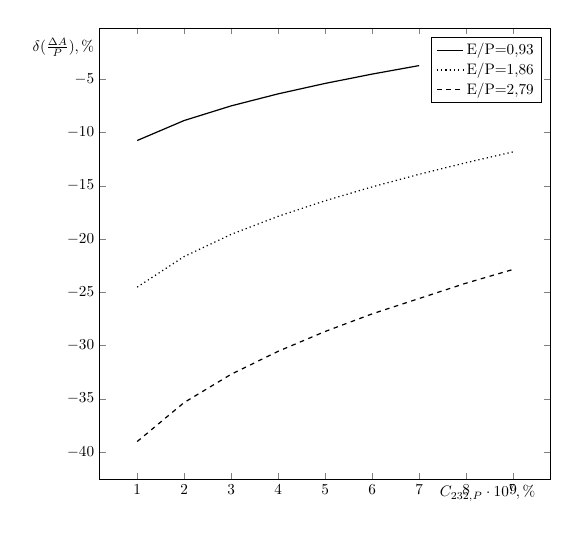
\begin{tikzpicture}[,
scale=0.55]
\begin{axis}[
  xlabel style = {{at={(axis description cs:.86,0)}}},
  ylabel = {$\delta(\frac{\Delta A}{P}), \%$},
  ylabel style = {{at={(axis description cs:-0.08,.925)},rotate=270,anchor=south}},
  xlabel = {$C_{232,P}\cdot10^{7}, \%$},
  width=12cm, height=12cm
]

\addplot+[mark=none,
  solid, black, thick
] coordinates {
  (1.0, -10.75592874548788)
  (2.0, -8.877549872366233)
  (3.0000000000000004, -7.50289958013979)
  (4.0, -6.3729908570898814)
  (5.0, -5.39405720345885)
  (6.0, -4.517136753769094)
  (7.000000000000001, -3.717964070419745)
};
\addlegendentry{{}{E/P=0,93}}

\addplot+[mark=none,
  dotted, black, thick
] coordinates {
  (1.0, -24.523693715258393)
  (2.0, -21.64946440952475)
  (3.0000000000000004, -19.56910789260241)
  (4.0, -17.87302824962024)
  (5.0, -16.41089275400384)
  (6.0, -15.109277255129713)
  (7.000000000000001, -13.927405951747463)
  (8.0, -12.837656298351746)
  (9.000000000000002, -11.820833744285492)
};
\addlegendentry{{}{E/P=1,86}}

\addplot+[mark=none,
  dashed, black, thick
] coordinates {
  (1.0, -39.02572435708815)
  (2.0, -35.35744140949972)
  (3.0000000000000004, -32.707361682832236)
  (4.0, -30.547279725027575)
  (5.0, -28.687040100935018)
  (6.0, -27.03315569727767)
  (8.0, -24.149000859531828)
  (9.000000000000002, -22.860928202940787)
};
\addlegendentry{{}{E/P=2,79}}

\end{axis}
\end{tikzpicture}


\caption{{Зависимость экономии работы разделения от ПДК $^{232}$U в НОУ-продукте с обогащением до уровня 4,95\% для различных $\frac{E}{P}$.{\label{sw495}}}}
    \end{minipage}%
    \begin{minipage}{.5\textwidth}
      \centering
      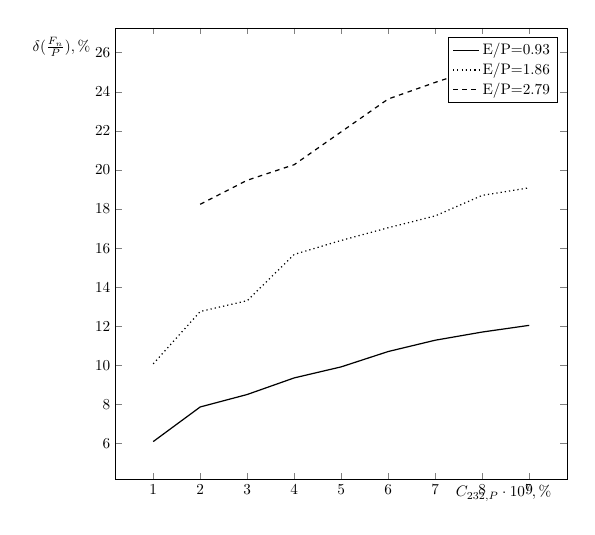
\begin{tikzpicture}[,
scale=0.55]
\begin{axis}[
  xlabel style = {{at={(axis description cs:.86,0)}}},
  ylabel = {$\delta(\frac{F_n}{P}), \%$},
  ylabel style = {{at={(axis description cs:-0.12,.925)},rotate=270,anchor=south}},
  xlabel = {$C_{232,P}\cdot10^{7}, \%$},
  width=12cm, height=12cm
]

\addplot+[mark=none,
  solid, black, thick
] coordinates {
  (1.0, 6.102609628967004)
  (2.0, 7.873257521230414)
  (3.0000000000000004, 8.510982187035465)
  (4.0, 9.359903696758797)
  (5.0, 9.924557345258734)
  (6.0, 10.709375471912841)
  (7.000000000000001, 11.287587970677283)
  (8.0, 11.705810902202751)
  (9.000000000000002, 12.048111265678951)
};
\addlegendentry{{}{E/P=0.93}}

\addplot+[mark=none,
  dotted, black, thick
] coordinates {
  (1.0, 10.07679447624098)
  (2.0, 12.756640615222503)
  (3.0000000000000004, 13.309773249935485)
  (4.0, 15.676539853992955)
  (5.0, 16.39235800951654)
  (6.0, 17.041722793102686)
  (7.000000000000001, 17.64593776461374)
  (8.0, 18.69753065296348)
  (9.000000000000002, 19.08456096001587)
};
\addlegendentry{{}{E/P=1.86}}

\addplot+[mark=none,
  dashed, black, thick
] coordinates {
  (2.0, 18.241079567317232)
  (3.0000000000000004, 19.47072745723193)
  (4.0, 20.268597025731783)
  (6.0, 23.628111214220738)
  (7.000000000000001, 24.476747414958155)
  (8.0, 25.273745846887998)
  (9.000000000000002, 25.337305198229632)
};
\addlegendentry{{}{E/P=2.79}}

\end{axis}
\end{tikzpicture}

    \caption{{Зависимость экономии расхода природного урана от ПДК $^{232}$U в НОУ-продукте с обогащением до уровня 4,95\% для различных $\frac{E}{P}$.{\label{F0R495}}}}
\end{minipage}
\end{figure}


\begin{figure}[ht]
    \centering
    \begin{minipage}{.5\textwidth}
      \centering
      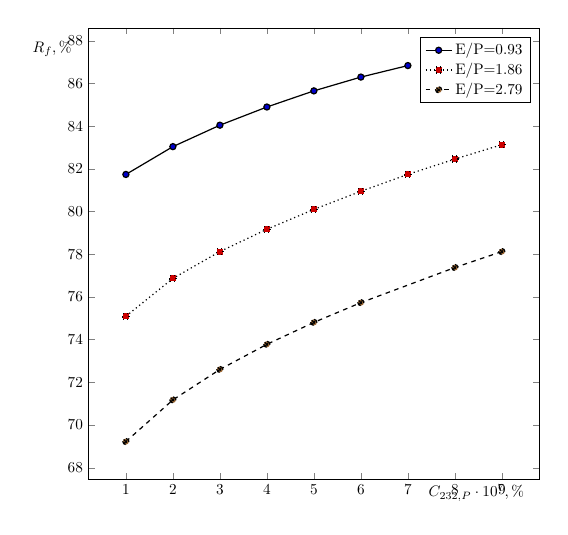
\begin{tikzpicture}[,
scale=0.55]
\begin{axis}[
  xlabel style = {{at={(axis description cs:.86,0)}}},
  ylabel = {$R_{f}, \%$},
  ylabel style = {{at={(axis description cs:-0.08,.925)},rotate=270,anchor=south}},
  xlabel = {$C_{232,P}\cdot10^{7}, \%$},
  width=12cm, height=12cm
]

\addplot+[
  solid, black, thick
] coordinates {
  (1.0, 81.73497884138504)
  (2.0, 83.03778477520555)
  (3.0000000000000004, 84.04194826713017)
  (4.0, 84.89394805905036)
  (5.0, 85.64964216184214)
  (6.0, 86.29627615264738)
  (7.000000000000001, 86.83475753524942)
};
\addlegendentry{{}{E/P=0.93}}

\addplot+[
  dotted, black, thick
] coordinates {
  (1.0, 75.09103641667504)
  (2.0, 76.86408581728926)
  (3.0000000000000004, 78.1230950450531)
  (4.0, 79.16703478387757)
  (5.0, 80.0973214088445)
  (6.0, 80.94802830843058)
  (7.000000000000001, 81.73831087619449)
  (8.0, 82.45610633767066)
  (9.000000000000002, 83.12799096181396)
};
\addlegendentry{{}{E/P=1.86}}

\addplot+[
  dashed, black, thick
] coordinates {
  (1.0, 69.22294832705394)
  (2.0, 71.17489372337026)
  (3.0000000000000004, 72.60072511995082)
  (4.0, 73.77803561909946)
  (5.0, 74.80542388393039)
  (6.0, 75.73053709257948)
  (8.0, 77.37433736075826)
  (9.000000000000002, 78.12192420776128)
};
\addlegendentry{{}{E/P=2.79}}

\end{axis}
\end{tikzpicture}


      \caption{{Зависимость степени извлечения $^{235}$U от ПДК $^{232}$U в НОУ-продукте с обогащением до уровня 4,95\% для различных $\frac{E}{P}$.{\label{ex495}}}}
    \end{minipage}%
    \begin{minipage}{.5\textwidth}
      \centering
      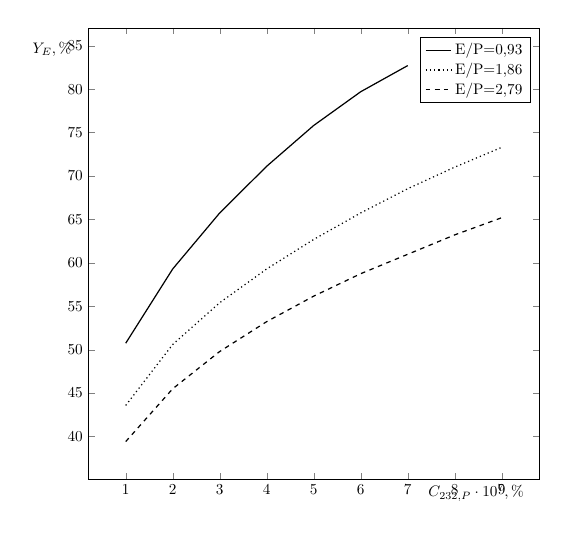
\begin{tikzpicture}[,
scale=0.55]
\begin{axis}[
  xlabel style = {{at={(axis description cs:.86,0)}}},
  ylabel = {$Y_{E}, \%$},
  ylabel style = {{at={(axis description cs:-0.08,.925)},rotate=270,anchor=south}},
  xlabel = {$C_{232,P}\cdot10^{7}, \%$},
  width=12cm, height=12cm
]

\addplot+[mark=none,
  solid, black, thick
] coordinates {
  (1.0, 50.745320366220234)
  (2.0, 59.30149726322195)
  (3.0000000000000004, 65.7519664106782)
  (4.0, 71.12954522207238)
  (5.0, 75.82763880377078)
  (6.0, 79.7135693705535)
  (7.000000000000001, 82.72543981227668)
};
\addlegendentry{{}{E/P=0,93}}

\addplot+[mark=none,
  dotted, black, thick
] coordinates {
  (1.0, 43.577905794327634)
  (2.0, 50.60187689534774)
  (3.0000000000000004, 55.41327633341921)
  (4.0, 59.30149726322195)
  (5.0, 62.69903149138577)
  (6.0, 65.75196641067834)
  (7.000000000000001, 68.5430309981216)
  (8.0, 71.02486897820552)
  (9.000000000000002, 73.30720710112764)
};
\addlegendentry{{}{E/P=1,86}}

\addplot+[mark=none,
  dashed, black, thick
] coordinates {
  (1.0, 39.414574744906304)
  (2.0, 45.501187547358626)
  (3.0000000000000004, 49.79017656124783)
  (4.0, 53.23340118139871)
  (5.0, 56.16715278135177)
  (6.0, 58.753339802423696)
  (8.0, 63.222220423599175)
  (9.000000000000002, 65.20220176963932)
};
\addlegendentry{{}{E/P=2,79}}

\end{axis}
\end{tikzpicture}


      \caption{{Зависимость степени извлечения $^{235}$U из регенерата от ПДК $^{232}$U в НОУ-продукте с обогащением до уровня 4,95\% для различных $\frac{E}{P}$.{\label{exR495}}}}
\end{minipage}
\end{figure}


Анализ представленных зависимостей рис. \ref{sw44}-\ref{exR495} позволяет сделать вывод о том, что эффективность предложенной каскадной схемы с точки зрения её основных интегральных характеристик в существенной мере зависит внешних условий. Например, экономия природного урана в цикле возрастает при увеличении отношения E/P. С другой стороны, в этом же случае растёт перерасход работы разделения в цикле и падают степени извлечения $^{235}U$ как из самого регенерата, так и в целом в схеме. Это означает, что выбор величины E/P, которая фактически определяет расход регенерированного урана в топливном цикле может стать предметом решения отдельной оптимизационной задачи, направленной на минимизацию издержек и экономию сырьевых материалов в цикле. 
Отметим, что из характера представленных кривых следует, что уменьшение допустимого предела по концентрации изотопа $^{232}$U в продукте также значительно влияет на интегральные характеристики каскадной схемы. В частности, для всех рассмотренных значений $E/P$ величина перерасхода работы разделения уменьшалась примерно вдвое в диапазоне изменения предельной концентрации $^{232}U$ в товарном НОУ от $1\cdot10^{-7}$\% до $1\cdot10^{-6}$\%. Также с ростом предельной концентрации $^{232}U$ в товарном НОУ на десятки процентов возрастали величины $Y_f$ и $Y_{E}$. Это означает, что уменьшение допустимой концентрации $^{232}$U в продукте при фиксированном отношении $E/P$ обусловливает ухудшение всех рассмотренных интегральных характеристик каскадной схемы. 

Для других величин обогащения $^{235}$U получены результаты, показавшие качественно аналогичные закономерности изменения интегральных характеристик каскадной схемы при различных условиях. 

Таким образом, полученные результаты позволяют сделать вывод о принципиальной применимости схемы двойного каскада с НОУ-разбавителем для решения задачи обогащения регенерированного урана в условиях многократного рецикла и в широком диапазоне изменения внешних условий задачи.    


\section{Общие выводы по результатам анализа схемы двойного каскада с НОУ-разбавителем}

\begin{enumerate}
    \item Предложена модификация двойного каскада с использованием дополнительного каскада для наработки НОУ-разбавителя для обогащения регенерированного урана различного состава в условиях многократного рецикла, позволяющая решить задачу обогащения регенерированного урана с одновременным выполнением условий на концентрации чётных изотопов в товарном НОУ и обеспечения условия полного использования регенерированного урана, поступившего в обогащение.
    \item Разработана оригинальная методика расчёта и оптимизации параметров предложенной каскадной схемы по различными критериям эффективности (каскады смоделированы на основе R-каскада). С использованием разработанной методики реализован компьютерный код, позволивший провести серию вычислительных экспериментов с целью оценки эффективности каскадной схемы при её оптимизации по различным критериям. По результатам проведенных численных исследований показано, что:
    \begin{itemize}
    \item схема применима для обогащения регенерированного урана в условиях многократного рецикла урана в топливе легководных реакторов, поскольку позволяет получать продукт, отвечающий всем требованиям на концентрации четных изотопов для регенерата различного исходного состава, включая случаи, когда исходное содержание $^{232}$U в регенерата в несколько раз превышает допустимые значения для товарного НОУ;
    \item показано, что с использованием предложенной схемы даже для составов с относительно высоким содержанием чётных изотопов возможно добиться экономии природного урана на уровне 15\% и выше при практически нулевом перерасходе или даже экономии затрат работы разделения;
    \item схема показывает свою устойчивость в условиях изменения внешних ограничений и требований к получаемому продукту -- товарному НОУ;
    \item наиболее обоснованным критерием эффективности является величина затрат работы разделения. С другой стороны наилучший набор параметров схемы может зависеть от исходного состава обогащаемого регенерата, поэтому целесообразно для определения оптимальных условий обогащения того или иного состава регенерата осуществлять расчёт и оптимизацию параметров каскадной схемы с использованием всех рассмотренных критериев эффективности.
    \item эффективность предложенной каскадной схемы зависит от выбранного диапазона изменения концентрации $^{235}$U в потоке отбора каскада II -- $P_2$. Наилучшие наборы параметров каскадной схемы для каждого из критериев лежат в области, где $C_{235,{P_2}} > 20\%$. Это означает, что при практической реализации модифицированного двойного каскада целесообразно рассматривать возможность получения в отдельных потоках такой схемы концентраций $^{235}$U, превышающих 20\%, и, в первую очередь, в потоке $P_2$.
    \end{itemize}       
    \item схема позволяет отделить участки обогащения регенерированного урана (где разделительное оборудование будет подвержено загрязнению минорными изотопами) от каскадов, обогащающих не содержащий $^{232,236}$U природный уран или ОГФУ. 
     \item среди недостатков схемы можно отметить накопление побочно производимого отхода в виде отбора второго каскада (поток $P_2$). Стратегии дальнейшего обращения с данным отходом требуют отдельного анализа.

\end{enumerate}


\section{Рассмотрение возможностей утилизации легкой фракции второго каскада в схеме}

\subsection{Анализ возможности утилизации легкой фракции путем ее перемешивания с регенератом, поступающим на обогащение}

\subsubsection{Описание схемы двойного каскада с НОУ-разбавителем с возвратом потока $P_2$ в цикл}\label{P2ret}

В качестве модификации предложенной схемы двойного каскада с НОУ-разбавителем (рис. \ref{p2left}) предложен способ, позволяющий вернуть отход в виде потока $P_2$ в топливный цикл для производства товарного НОУ. Предложенный способ проиллюстрирован на рис. \ref{P2utilizationRing} и состоит в следующем.

\begin{figure}[ht]
    \centerfloat{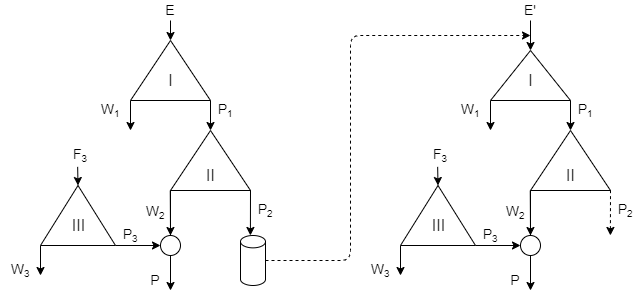
\includegraphics[scale=0.55]{cascades/P2utilizationRing}}
    \caption{Схема передачи загрязненной изотопом $^{232}$U фракции гексафторида урана в двойном каскаде от первой партии дообогащенного регенерированного урана к последующей. Обозначения: $E$ -- поток регенерированного урана; $P_1$ -- поток отбора первого каскада, выступающий питанием второго каскада; $W_1$ -- поток отвала первого каскада; $W_2$ -- поток тяжелой фракции (условный «отвал») второго каскада; $P_0$ -- поток НОУ-разбавителя; $P$ -- финальный продукт (товарный низкообогащенный уран (НОУ); $P_2$ -- поток отбора второго каскада, который подается на питание последующего двойного каскада, перемешиваясь с регенератом очередного рецикла}\label{P2utilizationRing}
\end{figure}

Учитывая, что каскадная схема рис. \ref{p2left} может быть применена для обогащения регенерата с относительно высоким исходным содержанием изотопа $^{232}$U, её можно использовать для вовлечения в производство обогащенного урана ранее полученного в ней же отхода в виде потока отбора второго каскада ($P_2$), загрязненного чётными изотопами. Для этого гексафторид урана из потока $P_2$ может быть перемешан с регенератом, полученным из следующей партии отработавшего топлива. Полученная в результате такого смешивания смесь будет отправлена на последующее обогащение в модифицированном двойном каскаде (рис. \ref{P2utilizationRing}), аналогичном представленному на рис. \ref{p2left}.

Подобный способ организации обогащения регенерированного урана призван замкнуть топливный цикл по урановой составляющей, вовлекая практически всю массу $^{235}$U из поступающего в обогащение регенерата. Единственным отходом производства останется ОГФУ, образующийся в отвале первого каскада (рис. \ref{P2utilizationRing}), который можно считать штатным отходом обогатительного производства с отработанными технологиями обращения и хранения. При этом после завершения производственного цикла останется невостребованной только та масса отхода (поток ${P_2}'$ на рис. \ref{P2utilizationRing})), которая будет образована после обогащения последней партии регенерата. Таким образом, описываемый подход к дообогащению регенерата урана в теории позволяет организовать возврат практически всей массы регенерированного урана в топливный цикл в течение всего жизненного цикла задействованного урана. Это должно обеспечить снижение потерь $^{235}$U на всем жизненном цикле уранового топлива.

Для проверки возможности и потенциальной эффективности использования предложенного способа организации обогащения регенерированного урана с возвратом в топливный цикл отхода в виде потока $P_2$ проведена серия вычислительных экспериментов с оценки интегральных показателей рассматриваемой каскадной схемы. Для этого была модифицирована методика расчёта и оптимизации каскадной схемы рис. \ref{p2left}, описанная в подразделе \ref{statement}. Изменения состояли в том, что при каждом расчёте обогащения регенерированного урана рассчитывали новый вариант состава питающей смеси регенерированного урана с учётом смешивания исходного регенерата, поступившего в обогащение и отхода ($P_2$), оставшегося после прошлого цикла обогащения. Новый состав поступающей в обогащение смеси рассчитывали по очевидной формуле:

\begin{equation} \label{Cie} 
    C_{i,E}=\frac{E_0}{E}{C_{i,{E_0}}} + \frac{P_2}{E}{C_{i,{P_2}}}
\end{equation}

где $E$ -- поток регенерированного урана полученный в результате смешивания потока исходного регенерата $E_0$ и отхода с предыдущего цикла обогащения $P_2$, $C_{i,E}$, $C_{i,{E_0}}$, $C_{i,{P_2}}$ -- концентрации $i$-го компонента в потоках $E$, $E_0$ и $P_2$, соответственно.     

Была рассмотрена следующая постановка задачи расчёта и оптимизации параметров каскадной схемы при способе организации обогащения регенерированного урана как на рис. \ref{P2utilizationRing})).

Задано:

\begin{itemize}
    \item величины $E_0$, $P_2$, $C_{i,{E_0}}$ и $C_{i,{P_2}}$; 
    \item коэффициент компенсации реактивности -- $K_{236}$;
    \item концентрации $C_{235,{W_1}}$ и $C_{235,{W_0}}$;
    \item коэффициент разделения на единичную разность массовых чисел $q_{0}$;
    \item предельно допустимое значение концентрации $C_{232,{P}}$;
    \item отношение потоков ${E_0}/P$;
    \item предельно допустимое отношение $\frac{C_{234,{P}}}{C_{235,{P}}}$. 
\end{itemize}

В процессе расчёта каскадной схемы необходимо определить:

\begin{itemize}
    \item величины потоков $P_0$, $W_0$, $P_1$, $W_1$, $P_2$, $W_2$ и концентрации всех компонентов в указанных потоках; 
    \item длины секций каждого из каскадов, определяемые величинами $N_1$, $f_1$, $N_2$, $f_2$, $N_3$, $f_3$ и прочие внутренние параметры каждого из каскадов;
    \item концентрации компонентов в потоке финального продукта -- товарном НОУ -- $C_{i,P}$.
\end{itemize}

При этом найденные величины параметров каскадов должны отвечать наилучшему значению выбранного критерия эффективности.  

Для реализации методики расчёту и оптимизации параметров каскадной схемы рис. \ref{P2utilizationRing})) для сформулированной выше задачи был адаптирован код, использовавшийся ранее для расчёта и оптимизации каскадной схемы рис. \ref{p2left}, реализующий описанный в \ref{statement} оригинальный алгоритм. В качестве критериев эффективности также рассмотрены величины $\frac{\Delta A}{P}$, $\delta(\frac{F_{NU}}{P})$, $Y_E$, а также минимум величины отхода каскада II.    

Вычислительные эксперименты проводили для следующих заданных величин параметров: 

\begin{itemize}
    \item обогащаемый регенерат соответствует составу 2 в таблицы \ref{is_compositions_2_5};
    \item $C_{235,{P}}=4,95\%$;
    \item $K_{236}=0,29$;
    \item $q_{0} = \sqrt[3]{1,2}$;
    \item $C_{235,{W_1}}=C_{235,{W_0}}=0,1\%$;
    \item ${(C_{232,P})}_{lim}=5\cdot10^{-7}\%$;
    \item $\frac{E_0}{P}=0,93$.
\end{itemize}

При моделировании возврата отхода от обогащения регенерированного урана в производство свежего НОУ исходили из того, что в процессе эксплуатация легководного реактора (например, ВВЭР-1000 или ВВЭР-1200) необходимо совершать так называемые перегрузки топлива, в рамках которых часть ТВС из активной зоны реактора удаляют, заменяя их новыми. При этом в пределах одного полного рецикла топлива в таком реакторе (примерно 7 лет) может быть осуществлено до семи частичных перегрузок. Последовательность перегрузок можно описать следующим образом. Из рассматриваемого исходного состава регенерата изготавливают сначала топливо для первой перегрузки. Далее, загрязненную фракцию от обогащения регенерата для первой перегрузки перемешивают с регенератом исходного состава для второй перегрузки и направляют на последующее обогащение для получения топлива следующей перегрузки и так далее. В итоге рассматривали 7 таких перегрузок. При расчёте параметров каскадной схемы для обогащения регенерата для каждой из перегрузок проводили также и оптимизацию с использованием описанного в \ref{statement} алгоритма. При этом был проведен цикл расчётов, в котором каждая из серий отличалась выбором критерия эффективности. Иными словами были проведены серии из расчётов параметров каскадной схемы для семи перегрузок, отличающиеся тем, что в каждой серии оптимизацию проводили только по одному критерию эффективности. Ниже представлены результаты проведенных вычислительных экспериментов и проведен их краткий анализ.

На рис. \ref{3} представлено изменение экономии природного урана при получении товарного НОУ для каждой из семи перегрузок и четырёх различных критериях эффективности. Как следует из анализа зависимостей, они близки и местами практически совпадают. Это можно объяснить тем, что данные критерии близки по своей сути. Например, максимум степени извлечения $^{235}$U из поступающего в обогащение регенерата должен приводить к необходимости использования минимальной массы $^{235}$U из природного сырья, что и выражается в уменьшении расхода природного сырья. В целом все кривые представляют собой возрастающие с ростом номера перегрузки функции, что отражает тот факт, что с каждой перегрузкой масса исходного регенерата возрастает одновременно с повышением концентрации $^{235}$U в нем, тем самым замещая собой природный уран.

На рис. \ref{4}-\ref{6} представлены, кривые отражающие оптимальные значения остальных критериев эффективности для каждой перегрузки. Как можно заметить общей тенденцией для всех случаев является снижение эффективности схемы по каждому из показателей. НАпример, можно видеть, что происходит уменьшение степени извлечения $^{235}$U из регенерата на каждой последующей перегрузке, что, по-видимому, обуславливает также и увеличение перерасхода работы разделения. Эти факторы являются следствием того, что с каждой перегрузкой повышаются концентрации чётных изотопов в питающем первый каскад регенерате и масса самого регенерата. Эти утверждения иллюстрируют рис. \ref{7}-\ref{10}.   


\begin{figure}[ht]
    \centering
    \begin{minipage}{.5\textwidth}
      \centering
      \begin{tikzpicture}[,
scale=0.95]
\begin{axis}[
  xlabel style = {{at={(axis description cs:.86,0)}}},
  ylabel = {$\delta(\frac{F_{NU}}{P}), \%$},
  ylabel style = {{at={(axis description cs:-0.08,.94)},rotate=270,anchor=south}},
  xlabel = {$i$},
  width=16cm, height=16cm, xtick={1,2,3,4,5,6,7}
]

\addplot+[
  solid, green, thin
] coordinates {
  (1.0, 9.60224940765123)
  (2.0, 10.471964607421514)
  (3.0, 10.328677265019726)
  (4.0, 10.937722799772365)
  (5.0, 11.551073258460454)
  (6.0, 11.482634526238378)
  (7.0, 11.495414262020132)
};
\addlegendentry{{}{$(Y_f)_\text{max}$}}

\addplot+[
  dotted, red, thick
] coordinates {
  (1.0, 9.60224940765123)
  (2.0, 10.471964607421514)
  (3.0, 10.328677265019726)
  (4.0, 10.937722799772365)
  (5.0, 11.551073258460454)
  (6.0, 11.482634526238378)
  (7.0, 11.495414262020132)
};
\addlegendentry{{}{$(Y_{E})_\text{max}$}}

\addplot+[
  dashed, black, thick
] coordinates {
  (1.0, 9.758344663807906)
  (2.0, 10.377586059230682)
  (3.0, 10.148945832377942)
  (4.0, 11.036603656094378)
  (5.0, 11.596700175896046)
  (6.0, 11.502422364899322)
  (7.0, 11.5042389394856)
};
\addlegendentry{{}{$(\delta(\frac{\Delta A}{P}))_\text{min}$}}

\addplot+[
  dashdotted, brown, thick
] coordinates {
  (1.0, 10.428757919569875)
  (2.0, 11.091940883100326)
  (3.0, 11.132231272182302)
  (4.0, 11.940825541138867)
  (5.0, 12.240045586112991)
  (6.0, 12.233596137265634)
  (7.0, 12.281186997924387)
};
\addlegendentry{{}{$(\delta(\frac{F_{NU}}{P}))_\text{min}$}}

\addplot+[
  solid, teal, thin
] coordinates {
  (1.0, 9.758344663807906)
  (2.0, 10.377586059230682)
  (3.0, 10.148945832377942)
  (4.0, 11.415331124937522)
  (5.0, 11.403205816515582)
  (6.0, 11.411528711119201)
  (7.0, 11.462271406331004)
};
\addlegendentry{{}{$(\frac{P_2}{P})_\text{min}$}}

\end{axis}
\end{tikzpicture}


      \caption{{Зависимость удельного расхода природного урана в двойном каскаде с замыканием в зависимости от номера перегрузки для обогащения 4,95\% для различных критериев эффективности.{\label{3}}}}
    \end{minipage}%
    \begin{minipage}{.5\textwidth}
      \centering
      \begin{tikzpicture}[,
scale=0.95,
scale=0.95]
\begin{axis}[
  xlabel style = {{at={(axis description cs:.86,0)}}},
  ylabel = {$R_{RepU}, \%$},
  ylabel style = {{at={(axis description cs:-0.08,.925)},rotate=270,anchor=south}},
  xlabel = {$i$},
  width=16cm, height=16cm
]

\addplot+[
  solid, black, thick
] coordinates {
  (1.0, 72.8241808435042)
  (2.0, 66.68566594907492)
  (3.0, 58.35228156487533)
  (4.0, 56.643420943442365)
  (5.0, 56.21679099162951)
  (6.0, 54.184876916297)
  (7.0, 52.553320781875414)
};
\addlegendentry{{}{$(R_f)_\text{max}$}}

\addplot+[
  dotted, black, thick
] coordinates {
  (1.0, 72.8241808435042)
  (2.0, 66.68566594907492)
  (3.0, 58.35228156487533)
  (4.0, 56.643420943442365)
  (5.0, 56.21679099162951)
  (6.0, 54.184876916297)
  (7.0, 52.553320781875414)
};
\addlegendentry{{}{$(R_{RepU})_\text{max}$}}

\addplot+[
  dashed, black, thick
] coordinates {
  (1.0, 73.82998902426432)
  (2.0, 66.64446941870102)
  (3.0, 57.19448148394325)
  (4.0, 56.67546946948041)
  (5.0, 56.226760998555434)
  (6.0, 54.188337945615274)
  (7.0, 52.5546392882073)
};
\addlegendentry{{}{$(\delta(\frac{\Delta U}{P}))_\text{min}$}}

\addplot+[
  dashdotted, black, thick
] coordinates {
  (1.0, 73.75583473104476)
  (2.0, 66.44811675745768)
  (3.0, 58.2996545335423)
  (4.0, 57.50685876177931)
  (5.0, 55.96223087076096)
  (6.0, 53.951506368752476)
  (7.0, 52.3277838935582)
};
\addlegendentry{{}{$(\delta(\frac{F_{NU}}{P}))_\text{min}$}}

\addplot+[
  solid, red, thick
] coordinates {
};
\addlegendentry{{}{$(C_{232,P})_\text{min}$}}

\addplot+[
  solid, blue, thick
] coordinates {
};
\addlegendentry{{}{$(C_{236,P})_\text{min}$}}

\addplot+[
  solid, brown, thick
] coordinates {
  (1.0, 73.82998902426432)
  (2.0, 66.64446941870102)
  (3.0, 57.19448148394325)
  (4.0, 58.460758694419646)
  (5.0, 56.177556015313)
  (6.0, 54.169304400774244)
  (7.0, 52.547895768556174)
};
\addlegendentry{{}{$(\frac{P_2}{P})_\text{min}$}}

\end{axis}
\end{tikzpicture}


\caption{{Степень извлечения $^{235}$U из исходного регенерата в двойном каскаде с замыканием в зависимости от номера перегрузки для обогащения 4,95\% для различных критериев эффективности.{\label{4}}}}
\end{minipage}
\end{figure}



\begin{figure}[ht]
    \centering
    \begin{minipage}{.5\textwidth}
      \centering
      \begin{tikzpicture}[,
scale=0.95,
scale=0.95]
\begin{axis}[
  xlabel style = {{at={(axis description cs:.86,0)}}},
  ylabel = {$\delta(\frac{P_{2}}{P}), \%$},
  ylabel style = {{at={(axis description cs:-0.08,.94)},rotate=270,anchor=south}},
  xlabel = {$i$},
  width=16cm, height=16cm, xtick={1,2,3,4,5,6,7}
]

\addplot+[
  solid, green, thin
] coordinates {
  (1.0, 1.0810960189992584)
  (2.0, 1.6146633333341598)
  (3.0, 2.3687024775347747)
  (4.0, 3.159113715125525)
  (5.0, 3.0809753572386254)
  (6.0, 3.3558969337102944)
  (7.0, 3.621806533418627)
};
\addlegendentry{{}{$(Y_f)_\text{max}$}}

\addplot+[
  dotted, red, thick
] coordinates {
  (1.0, 1.0810960189992584)
  (2.0, 1.6146633333341598)
  (3.0, 2.3687024775347747)
  (4.0, 3.159113715125525)
  (5.0, 3.0809753572386254)
  (6.0, 3.3558969337102944)
  (7.0, 3.621806533418627)
};
\addlegendentry{{}{$(Y_{E})_\text{max}$}}

\addplot+[
  dashed, black, thick
] coordinates {
  (1.0, 0.9191318565385409)
  (2.0, 1.5995427357743446)
  (3.0, 2.4336632372639344)
  (4.0, 3.1886436788896333)
  (5.0, 3.0921075113377343)
  (6.0, 3.3608476613695917)
  (7.0, 3.6241033759848253)
};
\addlegendentry{{}{$(\delta(\frac{\Delta A}{P}))_\text{min}$}}

\addplot+[
  dashdotted, brown, thick
] coordinates {
  (1.0, 0.9234810348382065)
  (2.0, 1.612721145807963)
  (3.0, 2.3724712118887568)
  (4.0, 2.9252605855990694)
  (5.0, 3.0737574380632946)
  (6.0, 3.3714004647467988)
  (7.0, 3.6482779696747203)
};
\addlegendentry{{}{$(\delta(\frac{F_{NU}}{P}))_\text{min}$}}

\addplot+[
  solid, teal, thin
] coordinates {
  (1.0, 0.9191318565385409)
  (2.0, 1.5995427357743446)
  (3.0, 2.4336632372639344)
  (4.0, 2.7304942598358695)
  (5.0, 3.036681544811821)
  (6.0, 3.3363360013335974)
  (7.0, 3.6127481585062196)
};
\addlegendentry{{}{$(\frac{P_2}{P})_\text{min}$}}

\end{axis}
\end{tikzpicture}


      \caption{{Зависимость величины удельного отхода (на единицу продукта) в зависимости от номера перегрузки для обогащения 4,95\% для различных критериев эффективности.{\label{5}}}}
    \end{minipage}%
    \begin{minipage}{.5\textwidth}
      \centering
      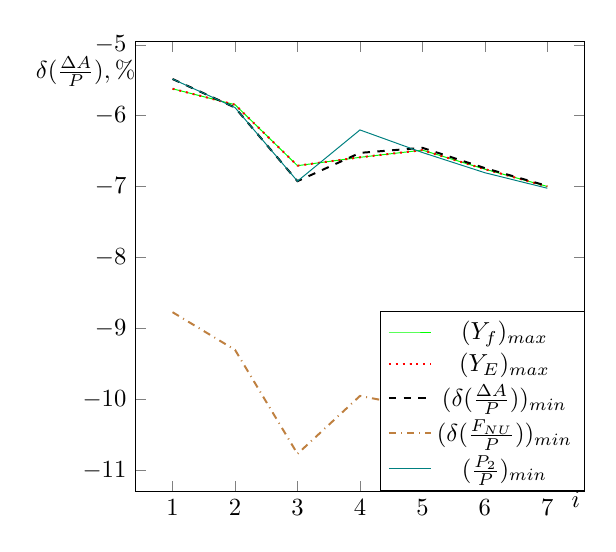
\begin{tikzpicture}[,
scale=0.89]
\begin{axis}[
  xlabel style = {{at={(axis description cs:.98,0.02)}}},
  ylabel = {$\delta(\frac{\Delta A}{P}), \%$},
  ylabel style = {{at={(axis description cs:-0.11,.88)},rotate=270,anchor=south}},
  xlabel = {$i$},
  width=8cm, height=8cm, xtick={1,2,3,4,5,6,7}, legend style={at={(1,0)},anchor=south east}
]

\addplot+[mark=none,
  solid, green, thin
] coordinates {
  (1.0, -5.619564224321039)
  (2.0, -5.84441657242741)
  (3.0, -6.704917867424845)
  (4.0, -6.586866390801599)
  (5.0, -6.485554729454776)
  (6.0, -6.754284481908828)
  (7.0, -6.998000929961407)
};
\addlegendentry{{}{$(Y_f)_\text{max}$}}

\addplot+[mark=none,
  dotted, red, thick
] coordinates {
  (1.0, -5.619564224321039)
  (2.0, -5.84441657242741)
  (3.0, -6.704917867424845)
  (4.0, -6.586866390801599)
  (5.0, -6.485554729454776)
  (6.0, -6.754284481908828)
  (7.0, -6.998000929961407)
};
\addlegendentry{{}{$(Y_{E})_\text{max}$}}

\addplot+[mark=none,
  dashed, black, thick
] coordinates {
  (1.0, -5.482150178426482)
  (2.0, -5.884813687357447)
  (3.0, -6.923308229121754)
  (4.0, -6.524186589001574)
  (5.0, -6.4527000666451135)
  (6.0, -6.739088245807983)
  (7.0, -6.991066392896656)
};
\addlegendentry{{}{$(\delta(\frac{\Delta A}{P}))_\text{min}$}}

\addplot+[mark=none,
  dashdotted, brown, thick
] coordinates {
  (1.0, -8.771994897379303)
  (2.0, -9.303209789751323)
  (3.0, -10.770438360555245)
  (4.0, -9.953392791027085)
  (5.0, -10.122163189828624)
  (6.0, -10.411774829351534)
  (7.0, -10.654096806225095)
};
\addlegendentry{{}{$(\delta(\frac{F_{NU}}{P}))_\text{min}$}}

\addplot+[mark=none,
  solid, teal, thin
] coordinates {
  (1.0, -5.482150178426482)
  (2.0, -5.884813687357447)
  (3.0, -6.923308229121754)
  (4.0, -6.2006153993959785)
  (5.0, -6.519171025702167)
  (6.0, -6.804418040883925)
  (7.0, -7.023084861927327)
};
\addlegendentry{{}{$(\frac{P_2}{P})_\text{min}$}}

\end{axis}
\end{tikzpicture}


\caption{{Зависимость экономии работы разделения в зависимости от номера перегрузки для обогащения 4,95\% для различных критериев оптимальности.{\label{6}}}}
\end{minipage}
\end{figure}

\begin{figure}[ht]
    \centering
    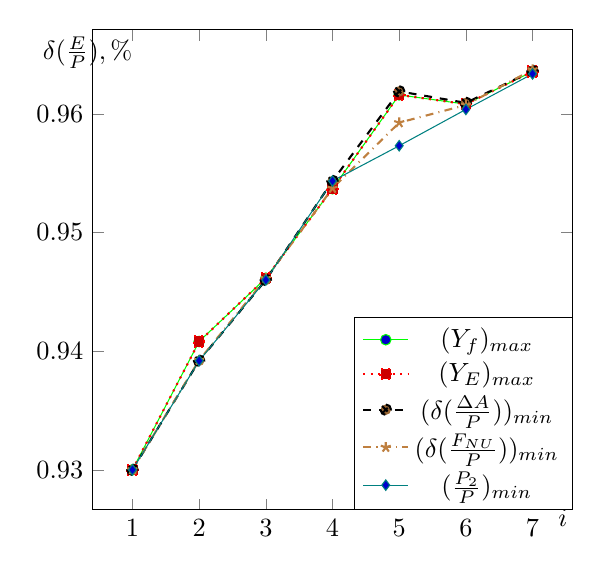
\begin{tikzpicture}[,
scale=0.95]
\begin{axis}[
  xlabel style = {{at={(axis description cs:.98,0.02)}}},
  ylabel = {$\delta(\frac{E}{P}), \%$},
  ylabel style = {{at={(axis description cs:-0.01,.9)},rotate=270,anchor=south}},
  xlabel = {$i$},
  width=8cm, height=8cm, xtick={1,2,3,4,5,6,7}, legend style={at={(1,0)},anchor=south east}
]

\addplot+[
  solid, green, thin
] coordinates {
  (1.0, 0.93)
  (2.0, 0.9408109601899927)
  (3.0, 0.9461466333333417)
  (4.0, 0.9536870247753478)
  (5.0, 0.9615911371512553)
  (6.0, 0.9608097535723863)
  (7.0, 0.9635589693371029)
};
\addlegendentry{{}{$(Y_f)_\text{max}$}}

\addplot+[
  dotted, red, thick
] coordinates {
  (1.0, 0.93)
  (2.0, 0.9408109601899927)
  (3.0, 0.9461466333333417)
  (4.0, 0.9536870247753478)
  (5.0, 0.9615911371512553)
  (6.0, 0.9608097535723863)
  (7.0, 0.9635589693371029)
};
\addlegendentry{{}{$(Y_{E})_\text{max}$}}

\addplot+[
  dashed, black, thick
] coordinates {
  (1.0, 0.93)
  (2.0, 0.9391913185653855)
  (3.0, 0.9459954273577434)
  (4.0, 0.9543366323726394)
  (5.0, 0.9618864367888964)
  (6.0, 0.9609210751133774)
  (7.0, 0.963608476613696)
};
\addlegendentry{{}{$(\delta(\frac{\Delta A}{P}))_\text{min}$}}

\addplot+[
  dashdotted, brown, thick
] coordinates {
  (1.0, 0.93)
  (2.0, 0.9392348103483821)
  (3.0, 0.9461272114580797)
  (4.0, 0.9537247121188877)
  (5.0, 0.9592526058559907)
  (6.0, 0.960737574380633)
  (7.0, 0.963714004647468)
};
\addlegendentry{{}{$(\delta(\frac{F_{NU}}{P}))_\text{min}$}}

\addplot+[
  solid, teal, thin
] coordinates {
  (1.0, 0.93)
  (2.0, 0.9391913185653855)
  (3.0, 0.9459954273577434)
  (4.0, 0.9543366323726394)
  (5.0, 0.9573049425983587)
  (6.0, 0.9603668154481183)
  (7.0, 0.963363360013336)
};
\addlegendentry{{}{$(\frac{P_2}{P})_\text{min}$}}

\end{axis}
\end{tikzpicture}


    \caption{Зависимость отношения потоков исходного регенерата и финального продукта (товарного НОУ) от номера перегрузки для обогащения 4,95\% для различных критериев эффективности.}\label{7}
\end{figure}



\begin{figure}[ht]
    \centering
    \begin{minipage}{.5\textwidth}
      \centering
      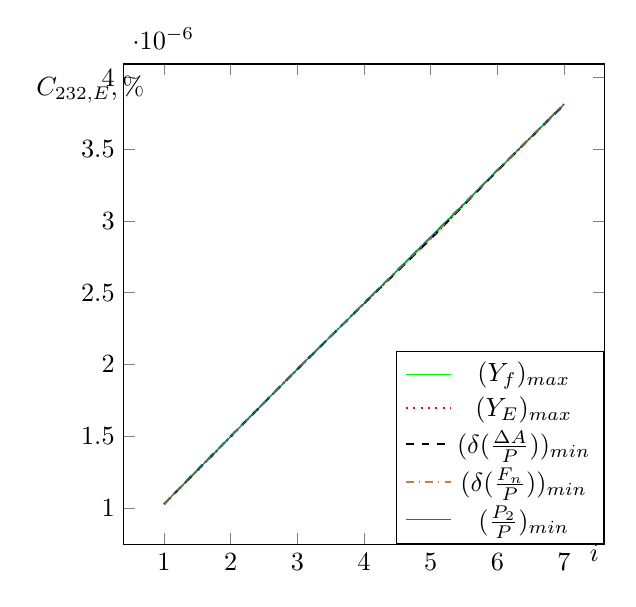
\begin{tikzpicture}[,
scale=0.95]
\begin{axis}[
  xlabel style = {{at={(axis description cs:.98,0.02)}}},
  ylabel = {$C_{232,E}, \%$},
  ylabel style = {{at={(axis description cs:-0.07,.9)},rotate=270,anchor=south}},
  xlabel = {$i$},
  width=8cm, height=8cm, xtick={1,2,3,4,5,6,7}, legend style={at={(1,0)},anchor=south east}
]

\addplot+[mark=none,
  solid, green, thin
] coordinates {
  (1.0, 1.0258e-6)
  (2.0, 1.4957859253750262e-6)
  (3.0, 1.9664961607465805e-6)
  (4.0, 2.4263137653178574e-6)
  (5.0, 2.8778904991462944e-6)
  (6.0, 3.3521276901753137e-6)
  (7.0, 3.8130792268330165e-6)
};
\addlegendentry{{}{$(Y_f)_\text{max}$}}

\addplot+[mark=none,
  dotted, red, thick
] coordinates {
  (1.0, 1.0258e-6)
  (2.0, 1.4957859253750262e-6)
  (3.0, 1.9664961607465805e-6)
  (4.0, 2.4263137653178574e-6)
  (5.0, 2.8778904991462944e-6)
  (6.0, 3.3521276901753137e-6)
  (7.0, 3.8130792268330165e-6)
};
\addlegendentry{{}{$(Y_{E})_\text{max}$}}

\addplot+[mark=none,
  dashed, black, thick
] coordinates {
  (1.0, 1.0258e-6)
  (2.0, 1.4983651087539599e-6)
  (3.0, 1.966794869704306e-6)
  (4.0, 2.424641617685412e-6)
  (5.0, 2.8770017284534706e-6)
  (6.0, 3.351739961430355e-6)
  (7.0, 3.812886476915959e-6)
};
\addlegendentry{{}{$(\delta(\frac{\Delta A}{P}))_\text{min}$}}

\addplot+[mark=none,
  dashdotted, brown, thick
] coordinates {
  (1.0, 1.0258e-6)
  (2.0, 1.4990615983803834e-6)
  (3.0, 1.967973359837115e-6)
  (4.0, 2.428311055154392e-6)
  (5.0, 2.8875886094436138e-6)
  (6.0, 3.355665432112993e-6)
  (7.0, 3.816382169516411e-6)
};
\addlegendentry{{}{$(\delta(\frac{F_n}{P}))_\text{min}$}}

\addplot+[mark=none,
  solid, teal, thin
] coordinates {
  (1.0, 1.0258e-6)
  (2.0, 1.4983651087539599e-6)
  (3.0, 1.966794869704306e-6)
  (4.0, 2.424641617685412e-6)
  (5.0, 2.8907700275574118e-6)
  (6.0, 3.3536492768045208e-6)
  (7.0, 3.8138187754759447e-6)
};
\addlegendentry{{}{$(\frac{P_2}{P})_\text{min}$}}

\end{axis}
\end{tikzpicture}


      \caption{{Зависимость концентрации $^{232}$U в исходном регенерате от номера перегрузки для обогащения 4,95\% для различных критериев эффективности.{\label{8}}}}
    \end{minipage}%
    \begin{minipage}{.5\textwidth}
      \centering
      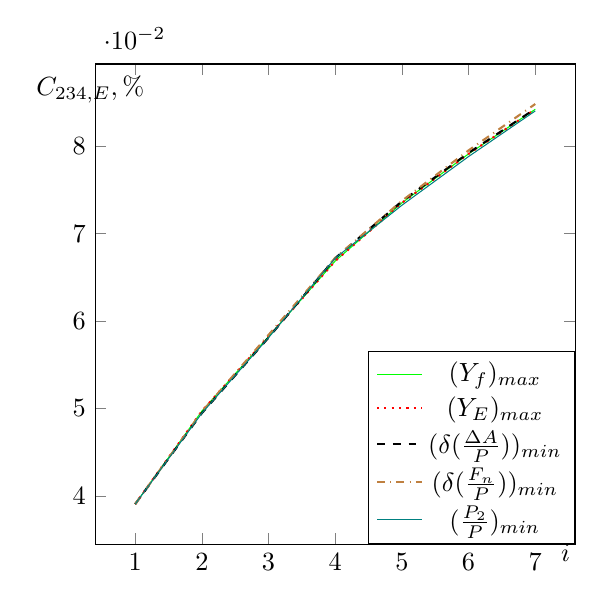
\begin{tikzpicture}[,
scale=0.95]
\begin{axis}[
  xlabel style = {{at={(axis description cs:.98,0.02)}}},
  ylabel = {$C_{234,E}, \%$},
  ylabel style = {{at={(axis description cs:-0.01,.9)},rotate=270,anchor=south}},
  xlabel = {$i$},
  width=8cm, height=8cm, xtick={1,2,3,4,5,6,7}, legend style={at={(1,0)},anchor=south east}
]

\addplot+[mark=none,
  solid, green, thin
] coordinates {
  (1.0, 0.039067000000000005)
  (2.0, 0.04970009905714201)
  (3.0, 0.05822673196432028)
  (4.0, 0.066871941585519)
  (5.0, 0.07352173483973685)
  (6.0, 0.07912564215270304)
  (7.0, 0.0842247287548398)
};
\addlegendentry{{}{$(Y_f)_\text{max}$}}

\addplot+[mark=none,
  dotted, red, thick
] coordinates {
  (1.0, 0.039067000000000005)
  (2.0, 0.04970009905714201)
  (3.0, 0.05822673196432028)
  (4.0, 0.066871941585519)
  (5.0, 0.07352173483973685)
  (6.0, 0.07912564215270304)
  (7.0, 0.0842247287548398)
};
\addlegendentry{{}{$(Y_{E})_\text{max}$}}

\addplot+[mark=none,
  dashed, black, thick
] coordinates {
  (1.0, 0.039067000000000005)
  (2.0, 0.04946841865210639)
  (3.0, 0.05810622920978174)
  (4.0, 0.06719588044561586)
  (5.0, 0.07370160217404174)
  (6.0, 0.07923292102134907)
  (7.0, 0.08429019401800651)
};
\addlegendentry{{}{$(\delta(\frac{\Delta A}{P}))_\text{min}$}}

\addplot+[mark=none,
  dashdotted, brown, thick
] coordinates {
  (1.0, 0.039067000000000005)
  (2.0, 0.049622790256222765)
  (3.0, 0.05841925622359249)
  (4.0, 0.06723365201075267)
  (5.0, 0.07375289742007517)
  (6.0, 0.07952538996328075)
  (7.0, 0.0848299502052639)
};
\addlegendentry{{}{$(\delta(\frac{F_n}{P}))_\text{min}$}}

\addplot+[mark=none,
  solid, teal, thin
] coordinates {
  (1.0, 0.039067000000000005)
  (2.0, 0.04946841865210639)
  (3.0, 0.05810622920978174)
  (4.0, 0.06719588044561586)
  (5.0, 0.0732483046560336)
  (6.0, 0.07882038255016108)
  (7.0, 0.08403644927222485)
};
\addlegendentry{{}{$(\frac{P_2}{P})_\text{min}$}}

\end{axis}
\end{tikzpicture}


\caption{{Зависимость концентрации $^{234}$U в исходном регенерате от номера перегрузки для обогащения 4,95\% для различных критериев эффективности.{\label{9}}}}
\end{minipage}
\end{figure}


\begin{figure}[ht]
    \centering
    \begin{minipage}{.5\textwidth}
      \centering
      \begin{tikzpicture}[,
scale=0.95,
scale=0.95,
scale=0.95,
scale=0.95]
\begin{axis}[
  xlabel style = {{at={(axis description cs:.86,0)}}},
  ylabel = {$C_{235,E}, \%$},
  ylabel style = {{at={(axis description cs:-0.05,.94)},rotate=270,anchor=south}},
  xlabel = {$i$},
  width=16cm, height=16cm, xtick={1,2,3,4,5,6,7}
]

\addplot+[
  solid, green, thin
] coordinates {
  (1.0, 1.0675000000000001)
  (2.0, 1.25936050072558)
  (3.0, 1.3865672666089406)
  (4.0, 1.5318691629561354)
  (5.0, 1.6160275951289529)
  (6.0, 1.6670280878275427)
  (7.0, 1.7186620013589922)
};
\addlegendentry{{}{$(Y_f)_\text{max}$}}

\addplot+[
  dotted, red, thick
] coordinates {
  (1.0, 1.0675000000000001)
  (2.0, 1.25936050072558)
  (3.0, 1.3865672666089406)
  (4.0, 1.5318691629561354)
  (5.0, 1.6160275951289529)
  (6.0, 1.6670280878275427)
  (7.0, 1.7186620013589922)
};
\addlegendentry{{}{$(Y_{E})_\text{max}$}}

\addplot+[
  dashed, black, thick
] coordinates {
  (1.0, 1.0675000000000001)
  (2.0, 1.2504710937036378)
  (3.0, 1.3836298662534239)
  (4.0, 1.5442795434551526)
  (5.0, 1.6209850102079988)
  (6.0, 1.669124592110755)
  (7.0, 1.7195891125167035)
};
\addlegendentry{{}{$(\delta(\frac{\Delta A}{P}))_\text{min}$}}

\addplot+[
  dashdotted, brown, thick
] coordinates {
  (1.0, 1.0675000000000001)
  (2.0, 1.251328369665262)
  (3.0, 1.3861900168691095)
  (4.0, 1.5325896194737838)
  (5.0, 1.6071563406244789)
  (6.0, 1.6656685168444958)
  (7.0, 1.7215649931745327)
};
\addlegendentry{{}{$(\delta(\frac{F_{NU}}{P}))_\text{min}$}}

\addplot+[
  solid, teal, thin
] coordinates {
  (1.0, 1.0675000000000001)
  (2.0, 1.2504710937036378)
  (3.0, 1.3836298662534239)
  (4.0, 1.5442795434551526)
  (5.0, 1.6007731300663814)
  (6.0, 1.6586814764166735)
  (7.0, 1.714997939379093)
};
\addlegendentry{{}{$(\frac{P_2}{P})_\text{min}$}}

\end{axis}
\end{tikzpicture}


      \caption{{Зависимость концентрации $^{235}$U в исходном регенерате от номера перегрузки для обогащения 4,95\% для различных критериев эффективности.{\label{10}}}}
    \end{minipage}%
    \begin{minipage}{.5\textwidth}
      \centering
      \begin{tikzpicture}[,
scale=0.95,
scale=0.95,
scale=0.95,
scale=0.95]
\begin{axis}[
  xlabel style = {{at={(axis description cs:.86,0)}}},
  ylabel = {$C_{236,E}, \%$},
  ylabel style = {{at={(axis description cs:-0.05,.94)},rotate=270,anchor=south}},
  xlabel = {$i$},
  width=16cm, height=16cm, xtick={1,2,3,4,5,6,7}
]

\addplot+[
  solid, green, thin
] coordinates {
  (1.0, 1.4458)
  (2.0, 1.5766817339001622)
  (3.0, 1.6449480750353955)
  (4.0, 1.740165734281792)
  (5.0, 1.7793867792372784)
  (6.0, 1.7880752865895622)
  (7.0, 1.8091968105027345)
};
\addlegendentry{{}{$(Y_f)_\text{max}$}}

\addplot+[
  dotted, red, thick
] coordinates {
  (1.0, 1.4458)
  (2.0, 1.5766817339001622)
  (3.0, 1.6449480750353955)
  (4.0, 1.740165734281792)
  (5.0, 1.7793867792372784)
  (6.0, 1.7880752865895622)
  (7.0, 1.8091968105027345)
};
\addlegendentry{{}{$(Y_{E})_\text{max}$}}

\addplot+[
  dashed, black, thick
] coordinates {
  (1.0, 1.4458)
  (2.0, 1.566303015750484)
  (3.0, 1.6429601127938132)
  (4.0, 1.7530908035297963)
  (5.0, 1.7826325779399714)
  (6.0, 1.7889860253626593)
  (7.0, 1.8094924815375841)
};
\addlegendentry{{}{$(\delta(\frac{\Delta A}{P}))_\text{min}$}}

\addplot+[
  dashdotted, brown, thick
] coordinates {
  (1.0, 1.4458)
  (2.0, 1.5488713796660698)
  (3.0, 1.61489559959293)
  (4.0, 1.6882125735298121)
  (5.0, 1.7165875952278868)
  (6.0, 1.7342271182454232)
  (7.0, 1.7552149382394835)
};
\addlegendentry{{}{$(\delta(\frac{F_{NU}}{P}))_\text{min}$}}

\addplot+[
  solid, teal, thin
] coordinates {
  (1.0, 1.4458)
  (2.0, 1.566303015750484)
  (3.0, 1.6429601127938132)
  (4.0, 1.7530908035297963)
  (5.0, 1.7591751938541251)
  (6.0, 1.7820375567783115)
  (7.0, 1.8074924037466793)
};
\addlegendentry{{}{$(\frac{P_2}{P})_\text{min}$}}

\end{axis}
\end{tikzpicture}


\caption{{Зависимость концентрации $^{236}$U в исходном регенерате от номера перегрузки для обогащения 4,95\% для различных критериев эффективности.{\label{11}}}}
\end{minipage}
\end{figure}


Итак, опираясь на результаты расчетов, можно сделать общие выводы касаемо двойного каскада с НОУ-разбавителем с возвратом потока $P_2$ в цикл (рис. \ref{p2left}):

\begin{enumerate}
    \item предложенный способ возврата возникающего при обогащении регенерат отхода в виде потока $P_2$ в производство НОУ применим для обогащения регенерированного урана в условиях многократного рецикла урана в топливе легководных реакторов, поскольку позволяет получать продукт, отвечающий всем требованиям решаемой задачи;
    \item схема позволяет почти полностью решить проблему долговременного хранения нештатного отхода ($P_2$) и связанные с этим затраты. Использование $P_2$ позволяет снизить потери $^{235}$U в процессе рециклирования и увеличить экономию природного урана по сравнению с открытым топливным циклом;
     \item возврат фракции отхода (потока $P_2$) в схему является причиной монотонного роста концентраций четных изотопов, что приводит к необходимости увеличения уровня обогащения получаемого НОУ и, тем самым, к росту затрат работы разделения, увеличению потока отхода при обогащении регенерата каждой последующей перегрузки, а также повышению концентрации изотопа $^{235}$U в НОУ-разбавителе ввиду необходимости компенсации влияния $^{236}$U. Данные факторы несколько снижают эффективность способа.
\end{enumerate}


\subsection{Анализ возможности использования легкой фракции второго каскада схемы двойного каскада с НОУ-разбавителем для получения дополнительной массы товарного НОУ}\label{indep_p2}

В работе предложен ещё один способ обращения с материалом, произодимом в потоке $P_2$ (рис. \ref{p2left}) и имеющим относительно высокие концентрации $^{235}$U (20\% и выше), который позволяет вовлечь этот материал в воспроизводство ядерного топлива. 

Идея предложенного способа проиллюстрирована на рис. \ref{P2utilization} и представляет чуть более сложную модификацию схемы рис. \ref{p2left}. Образовавшуюся во втором каскаде легкую фракцию $P_2$ разбавляют потоком обедненного урана ($F_D$), изотопный состав которого приведен в табл. \ref{DepU13} до такой концентрации $^{235}$U в получившейся смеси, который будет соответствовать эффективной концентрации $^{235}$U (то есть будет учитывать компенсацию $^{236}$U добавочным количеством $^{235}$U) в потоке свежего НОУ $F_{leu}$, произведенного из смеси природного урана. Затем, полученную смесь $P_2$ и $F_D$ дополнительно смешивают с низкообогащенным ураном $F_{leu}$, полученным обогащением природного урана, до достижения в получаемом продукте $P_{add}$ соответствия концентрации изотопа $^{232}$U заданному предельному значению -- $5\cdot10^{-7}$\%. Такая схема позволяет: (1) осуществить утилизацию побочного продукта $P_2$, образовавшегося в двойном модифицированном каскаде; (2) заместить некоторое количество НОУ ($F_{leu}$), произведенного из смеси природного урана, путем подмешивания к нему побочного продукта $P_2$ и обедненного урана. Иными словами, такой подход позволяет использовать выделенный в поток $P_2$ модифицированного двойного каскада $^{235}$U для получения дополнительной массы низкообогащенного урана, наряду с основной массой товарного НОУ, получаемого в потоке $P$. 

\begin{figure}[ht]
    \centerfloat{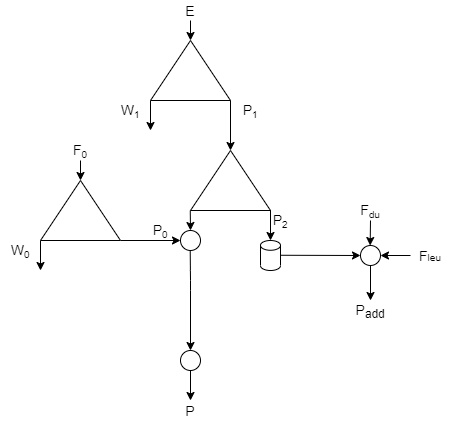
\includegraphics[scale=0.7]{cascades/P2utilization}}
    \caption{Схема независимого вовлечения загрязненной изотопом $^{232}$U фракции с разбавлением обедненным и природным ураном}\label{P2utilization}
\end{figure}

Алгоритм расчета для предлагаемой схемы следующий. Происходящее смешение потоков $P_2$, $F_D$ и $F_{leu}$, входящих в состав дополнительного продукта $P_{add}$, можно представить в виде системы уравнений баланса материальных потоков \ref{Padd_bal}. Затем, для контролируемых в получаемой смеси изотопов, можно сформулировать уравнения невязок (по целевым концентрациям изотопов в продукте) (\ref{dis_235_6_Padd}--\ref{dis_232_Padd}). Полученная система уравнений позволит вычислить отношения входящих в рузультирующий НОУ-продукт потоков $P_2$, $F_D$ и $F_{leu}$.

\begin{equation} \label{Padd_bal} 
  \begin{array}{l} {\quad \quad \quad \quad {P_{2}+F_D+F_{leu}=P_{add}},} \\ {P_{2}C_{i,P_{2}} + F_DC_{i,F_D} + F_{leu}C_{i,F_{leu}}  = P_{add}C_{i,P_{add}} ,\; i=1,2,...,m.} \end{array} 
\end{equation}


\begin{equation}
    \label{dis_235_6_Padd}
    \Delta_{236}=C_{235,P\textit{экв.}}-(C_{235,{P_{NU}}}+\Delta C_{235})
\end{equation}

, где $\Delta_{236}$ -- невязка по концентрации $^{235}$U в конечном НОУ-продукте, с учетом поправки на присутствие изотопа $^{236}$U. $C_{235,P\textit{экв.}}$ -- эквивалентная концентрация $^{235}$U в потоке товарного НОУ, $C_{235,{P_{NU}}}$ -- требуемая концентрация $^{235}$U в товарном НОУ без учёта компенсации влияния $^{236}$U, $\Delta C_{235}$ -- величина добавочного обогащения изотопа $^{235}$U для компенсации влияния $^{236}$U. 

\begin{equation}
\label{dis_232_Padd}
\Delta_{232}=\left|C_{232,P\textit{calc}}-C_{232,P\textit{given}}\right|
\end{equation}

, где $\Delta_{232}$ -- разница (по абсолютной величине) между рассчитанным значением концентрации $^{232}$U в конечном НОУ-продукте ($C_{232,P\textit{calc}}$) и заданной предельной величиной для концентрации этого изотопа ($C_{232,P\textit{given}}$).

Далее предлагается оценить долю замещаемого с помощью такой схемы НОУ-продукта на основе природного урана. Величина этой доли, соответствующая эффективности предлагаемой схемы, позволит сделать вывод о целесообразности применения такой схемы.  

\begin{table}[h]
    \centering
    \normalsize
    \begin{tabulary}{1.0\textwidth}{|c|c|c|c|c|c|}
        \hline Массовое число & 232 & 233 & 234 & 235 & 236\\
        \hline C, \% & 0 & 0 & $3,45\cdot10^{-4}$ & 0,13 & 0 \\\hline
    \end{tabulary}
\caption{{Изотопный состав ОГФУ-разбавителя.{\label{DepU13}}}}
\end{table}

Расчет схемы производился для составов №1 и №2 (см. постановку задачи в \ref{statement}), обогащаемых в схеме модифицированного двойного каскада для условий, сформулированных в \ref{statement}, для которых в продукте $P$ нарабатывается 1 т НОУ-продукта, а уровень обогащения $^{235}$U в $P_2$ составляет 20\% (изотопные составы взяты из таблиц \ref{2opt1_int}--\ref{2opt1}). Затем $P_2$ полученное в рассчитанном количестве (на 1 т НОУ-продукта модифицированного двойного каскада), а также ОГФУ, производимое из природного урана (состав приведен в табл. \ref{DepU13}) и имеющее концентрацию $^{235}$U 0,13\%), используются для получения $P_{add}$ (рис. \ref{P2utilization}) с ограничениями на предельно допустимую концентрацию $^{232}$U $5\cdot10^{-7}$\% (соответствует постановке задачи в \ref{statement}). Результаты вычислений представлены в таблице \ref{independent}.

\begin{table}[ht]
    \centering
    \normalsize\begin{tabulary}{1.0\textwidth}{|C|C|C|C|C|C|}
    \hline Состав № & $P_2$, кг & $F_D$, кг & $F_{leu}$, кг & $P_{add}$, кг & $P_{+}$, \% \\\hline 
    1 & 2,84 & 7,54 & 131,82 & 142,2 & 7,3 \\\hline
    2 & 1,96 & 4,47 & 197,77 & 204,2 & 3,15 \\\hline
    \end{tabulary}
    \caption{Результаты вовлечения $P_2$ в производство дополнительного НОУ-продукта. Обозначения: $(C_{232,P})_{lim}$ -- предельно допустимая концентрация $^{232}$U в дополнительно производимом на основе $P_2$ продукте; $P_{+}$ -- доля замещаемого посредством схемы НОУ-продукта, произведенного из природного урана. {\label{independent}}}
\end{table}

Значения масс $P_2$ в таблице \ref{independent} соответствуют образовавшемуся побочному продукту в процессе производства 1 тонны топлива из регенерата (примерно двух ТВС по $\approx$500 кг). А значения масс $P_{add}$ -- произведенному на основе $P_2$, ОГФУ и $F_{leu}$ дополнительному НОУ-продукту к полученной 1 т НОУ продукта на предыдущем шаге в схеме модифицированного двойного каскада.

Величина $P_{+}$, приведенная в табл. \ref{independent} соответствует доле замещаемого природного урана, используемого для получения свежего НОУ требуемого качества, и расчитывается как:
$P_{+} = \frac{P_2 + F_D}{P_{add}}$.

Иными словами, величина $P_{+}$, являясь основным характеристическим показателем схемы, соответствует доле смеси $P_2$ с ОГФУ в результирующем дополнительно произведенном НОУ-продукте. На эту величину можно заместить эквивалентный по нейтронно-физическим характеристикам НОУ, произведенный на основе природного урана, поэтому эта величина является важнейшим показателем целесообразности применения рассматриваемой схемы для утилизации нештатного «отхода», образовавшегося в легком конце второго каскада двухкаскадной схемы.

Эта величина по смыслу тождественна величинам экономии природного урана $\delta(\frac{F_{NU}}{P})$, а также экономии работы разделения $\delta(\frac{\Delta A}{P})$, взятым относительно референтной схемы трехпоточного каскада для обогащения природного урана.

Как видно из результатов табл. \ref{independent}, наиболее целесообразно использовать этот способ утилизации нештатного «отхода», образующегося в схеме на начальных рециклах, то есть при меньшей концентрации $^{232}$U, накопившейся в разделяемой смеси. Также  такая схема показывает пропорционально более высокую результативность (двукратно), при более высоких значениях предельно допустимой концентрации результирующего продукта -- $(C_{232,P})_{lim}$.

Как можно заключить из результатов, представленных в таблице \ref{independent}, предлагаемый способ использования $P_2$ через модификацию схемы двойного каскада с НОУ-разбавителем позволяет экономить дополнительное количество природного урана относительно двойного модифицированного каскада, в котором не предполагается задействование потока легкой фракции второго каскада. А эффект более значителен для случая, когда задействуется побочный продукт $P_2$ двойного каскада, образующийся на начальных стадиях рециклирования уранового топлива. В рассматриваемом случае -- состава регенерированного урана №1 (табл. \ref{independent}). Значение экономии природного урана за счет использования предложенной схемы соответствует доле $P_2$, смешанной с обедненным ураном $F_D$, до того, как он будет смешан с НОУ-разбавителем $F_{leu}$, полученным из природного урана. Важно заметить, что значение этой доли соответствует экономии работы разделения, которая, в случае отказа от использования $P_2$, была бы затрачена на прямое обогащение природного урана в ординарном каскада для производства аналогичного замещающего количества свежего НОУ-продукта.

Если оценить эффект предложенной схемы с точки зрения обеспечения реактора ядерным топливом, для варианта вовлечения $P_2$, образовавшегося в ходе обогащения на предыдущем шаге состава 1, получаем следующее. На каждые 7 ТВС ($\approx$3,5 т свежего НОУ топлива), скомпонованных из топлива, произведенного с помощью схемы модифицированного двойного состава, на основе $P_2$, ОГФУ и $F_{leu}$ можно произвести дополнительную ТВС ($\approx$0,5 т), в которой доля $P_2$+ОГФУ будет составлять 7,3\%, то есть в ходе производства этой дополнительной восьмой топливной сборки будет достигаться экономия природного урана, а также работы разделения на уровне 92,8\% за счет того, что 7,3\% конечного НОУ-продукта, составляющие эту ТВС, замещены $P_2$ и ОГФУ.

Полезно будет привести следующие оценки. Для современного легководного реактора, такого как, например, российский ВВЭР-1200 или европейский PWR, где активная зона состоит из более чем 150 тепловыделяющих сборок, взяв за основу предложенную схему, можно изготовить дополнительно 150/8$\approx$ 19 ТВС, сэкономив на их производство количество природного урана, требуемого для производства 19$\cdot$7,3\%$\approx$1,4 ТВС, что приблизительно соответствует 3,5$\cdot$1,4$\approx$5 тоннам уранового концентрата или 1000...2000 т урановой руды среднего сорта \cite{bekmanYaDERNAYaFIZIKA}.

Таким образом, предлагаемая схема задействования $P_2$, образовавшегося в результате работы модифицированного двойного каскада, позволяет добиться:
\begin{enumerate}
  \item Дополнительного сокращения доли потребляемого обедненного урана при сохранении возможности использования высокообогащенного побочного продукта;
  \item Обеспечение полного возврата массы регенерированного урана в топливный цикл;
  \item Повышения эффективности использования делящегося изотопа $^{235}$U из регенерата;
  \item Дополнительного увеличения экономии природного урана на производство единицы свежего топлива для загрузки легководного реактора.
\end{enumerate}

\subsection{Анализ возможности утилизации легкой фракции путем ее перемешивания с обедненным ураном и последующим обогащением}\label{triple_c}
\subsubsection{Каскадная схема с возвратом потока $P_2$ в цикл}

Другим предлагаемым способом утилизации загрязненной фракции (поток $P_2$) является многокаскадная схема, принципиальный вид которой изображён на рис. \ref{p2_withDepU} \cite{smirnovApplyingEnrichmentCapacities2018}.

\begin{figure}[ht]
    \centerfloat{
\includegraphics[scale=0.9]{cascades/p2_withDepU}}
    \caption{Тройной каскад для обогащения регенерированного урана. Обозначения: $E$ -- поток регенерированного урана; $P_1$ -- поток отбора первого каскада, выступающий питанием второго каскада; $P_2$ -- поток отбора второго каскада; $F_{D}$ -- поток ОГФУ-разбавителя, смешиваемого с $P_2$ перед подачей на вход третьего каскада; $W_1$ -- поток отвала первого каскада; $W_2$ -- поток тяжелой фракции (условный «отвал») второго каскада; $P_n$ -- поток НОУ-разбавителя; $P$ -- финальный продукт (товарный низкообогащенный уран (НОУ)), полученный смешиванием потоков $W_2$, $P_n$ и $P_3$, где $P_3$ -- отбор третьего каскада; $W_3$ -- отвал третьего каскада.}\label{p2_withDepU}
\end{figure}

Рассмотрим подробнее представленную на рис. \ref{p2_withDepU} каскадную схему. Её отличие от каскадной схемы рис. \ref{p2left} состоит в том, что поток легкой фракции второго каскада ($P_2$) перемешивают с обедненным ураном (поток $F_{D}$ на рис. \ref{p2_withDepU}, имеющий изотопный состав, приведенный в табл. \ref{DepU13}) и направляют на последующее обогащение в дополнительный каскад (каскад IV). Отношение потоков $P_2$ и $F_{D}$ определяют исходя из возможности получить на выходе из каскада IV НОУ, отвечающий всем требованиям по концентрациям чётных изотопов. При этом финальный продукт всей каскадной схемы формируют смешиванием трех потоков: $P_0$, $W_2$ и полученного при обогащении смеси потоков $P_2$ и $F_{D}$ потока $P_3$.

Проанализируем одну из возможных постановок задачи обогащения регенерированного урана в рассматриваемой каскадной схеме.

Задано:

\begin{itemize}
    \item концентрации компонентов в обогащаемом регенерированном уране -- $C_{i,{E}}$;
    \item концентрации компонентов в потоке обедненного урана -- $C_{i,{F_{D}}}$;
    \item отношение потоков $E/P$ -- (исходный регенерат)/(финальный продукт);
    \item величина концентрации $^{235}$U в потоке $W_{1}$ -- $C_{i,{W_1}}$;
    \item параметры одиночного разделительного элемента (центрифуги) - величины потока питания центрифуги ($l_{ГЦ}$) и коэффициента разделения, приходящегося на единичную разность массовых чисел ($q_{0}$);
    \item в случае использование моделей квазиидеального каскада или $R$-каскада необходимо либо непосредственное задание величины параметра $g_i$ (см. формулу \ref{GrindEQ__1_13_}, либо выбор пары компонентов, по которым должно быть выполнено условие несмешивания их относительных концентраций (подробнее см. Главу \ref{ch2_theory}).
\end{itemize}

Параметры каскадной схемы должны соответствовать требованиям, предъявляемым к получаемому товарному НОУ:

\begin{itemize}
    \item величина концентрации $^{235}$U в продукте (товарном НОУ, поток $P$ на схеме рис. \ref{p2left}) -- $C_{235,{P}}$;
    \item величины предельных концентраций изотопов $^{232}$U и $^{234}$U в конечном продукте $P$ -- $(C_{232,{P}})_{lim}$;
    \item величины предельно допустимого отношения концентраций изотопа $^{234}$U и $^{235}$U в конечном продукте $P$ -- ${C_{234,{P}}}/{C_{235,{P}}}$;
    \item вид функции $f(C_{236,P})$, в соответствии с которой рассчитывают конечную (эквивалентную) величину обогащения по $^{235}$U в продукте, с учётом компенсации присутствия $^{236}$U:
    $(C_{235,P})_\textit{экв.}=(C_{235,P})_\textit{прир.}+f(C_{236,P})$.    
\end{itemize}

Для определения параметров всей каскадной схемы необходим последовательный расчёт каждого из составляющих её каскадов. При расчёта параметров каждого из каскадов решали задачу проектировочного расчёта (см. Главу \ref{ch2_theory}). Это означало, что задаваемыми параметрами для каждого из каскадов в схеме были концентрации одного из изотопов в выходящих потоках этого каскада. Причём для всех каскадов удобно задать концентрации $^{235}$U.

Анализируя приведенную выше постановку задачи, набор заданных величин и учитывая использование модели $R$-каскада для расчёта параметров каждого из каскадов, можно прийти к следующим выводам. Для каждого из каскадов при заданных концентрациях в потоках питания, величине одного из внешних потоков ($F$, $P$ или $W$), параметрах одиночного разделительного элемента, для расчёта их параметров необходимо задать ещё 2 величины. Это могут быть полное число ступеней N и номер ступени подачи внешнего питания -- $f$, либо концентрации целевого компонента в потоках отбора и отвала каскада. Задание этих величин позволяет далее по соотношениям (\ref{GrindEQ__1_70_})-(\ref{GrindEQ__1_77_}) рассчитать все их внешние и внутренние параметры. Кроме того, ещё одной неизвестной величиной задачи является отношение потоков ${F_{D}}/{P_2}$.  Тем самым имеем ситуацию, при которой для последовательного расчёта параметров каждого из каскадов схемы необходимо задать в совокупности 9 величин, например: $C_{235,{W_1}}$, $C_{235,{P_1}}$, $C_{235,{W_2}}$, $C_{235,{P_2}}$, $C_{235,{W_0}}$, $C_{235,{P_0}}$, $C_{235,{W_3}}$, $C_{235,{P_3}}$ и ${F_{D}}/{P_2}$. 

Как следует из постановки задачи, по условию заданы только 2 из перечисленных выше величин: $C_{235,{W_1}}$, $C_{235,{W_0}}$. Оставшиеся 7 переменных подлежат определению в процессе расчёта. Однако для их нахождения можно записать только 2 независимых уравнения:

\begin{equation}
    \label{dis_235_6_triple}
    \Delta_{236}=0
\end{equation}

\begin{equation}
    \label{dis_232_triple}
    \Delta_{232}=0
\end{equation}

, где величины $\Delta_{232}$ и $\Delta_{236}$ определяют выполнение условия компенсации $^{236}$U и требований к максимально допустимой концентрации изотопа $^{232}$U в продукте и определяются соотношениями (\ref{dis_235_6}) и (\ref{dis_232}), соответственно.

Следует отметить, что в уравнения (\ref{dis_235_6_triple}), (\ref{dis_232_triple}) неявно входят все 7 неизвестных величин, поскольку они напрямую определяют параметры каждого из каскадов в схеме, а следовательно концентрации компонентов в формирующих конечный продукт потоках $P_0$, $W_2$, $P_3$ и величинах самих этих потоков. Таким образом, для замыкания системы уравнений (\ref{dis_235_6_triple})-(\ref{dis_232_triple}) необходимо задать 5 из неизвестных величин. Данные величины можно рассматривать в качестве оптимизационных переменных, поскольку их выбор будет напрямую определять величину выбранного критерия эффективности.


Величины $\Delta_{232}$ и $\Delta_{236}$ определяют выполнение условия компенсации $^{236}$U и требований к максимально допустимой концентрации изотопа $^{232}$U в продукте. Важно отметить, что уравнения системы (\ref{dis_235_6})-(\ref{dis_232}) отражают неявные зависимости величин концентраций изотопов $^{232}$U и $^{235}$U в потоке $P$ от искомых концентраций $C_{235,{W_2}}$, $C_{235,{P_0}}$. Это означает, что для расчёта величин $\Delta_{232}$ и $\Delta_{236}$ необходимо предварительно рассчитывать параметры каскадов II и III на основе некоторых начальных приближений для искомых концентраций $C_{235,{W_2}}$, $C_{235,{P_0}}$. Поэтому возможно только численное решение системы уравнений (\ref{dis_235_6})-(\ref{dis_232}) с расчётом параметров каскадов II и III на каждой итерации процедуры решения. Причём для расчета параметров каскадов I-III для каждой итерации решения системы (\ref{dis_235_6})-(\ref{dis_232}) необходимо отдельно численно решать системы уравнений вида (\ref{dis_235P})-(\ref{dis_235W}) для каждого из каскадов схемы. Решение систем уравнений обоих видов возможно осуществить одним из известных численных методов решения систем нелинейных уравнений. 

В рамках работы для решения возникающих в процессе расчёта параметров каскада систем нелинейных алгебраических уравнений (СНАУ) использован метод Trust-region (TRM) -- численный алгоритм для решения систем нелинейных уравнений, который базируется на определении области вокруг лучшего решения, в котором квадратичная модель аппроксимирует целевую функцию \cite{NumericalOptimization2006}. Реализация этого численного метода для решения целевой системы уравнений заимствована из открытой программной библиотеки семейства решателей JuliaNLSolvers \cite{mogensenJuliaNLSolversNLsolveJl2020}. Выбранный алгоритм позволяет с помощью автоматического дифференцирования вычислять матрицы Якоби и Гессе, не требуя их передачи в функцию (подпрограмму) решателя в явном виде, что является преимуществом этого алгоритма \cite{айда-задеБыстроеАвтоматическоеДифференцирование1989,revelsForwardModeAutomaticDifferentiation2016}.

Анализируя уравнения, описывающие модель <<квазиидеального>> тройного каскада, а также учитывая сформулированную выше постановку задачи, можно прийти к следующим заключениям. При заданных внешних условиях и требованиях к составу товарного НОУ, такая каскадная схема имеет 7 неизвестных переменных: 1) концентрация $^{235}$U в потоке $P_{1}$; 2) концентрация $^{235}$U в потоке $P_{2}$; 3) концентрация $^{235}$U в потоке $W_{2}$; 4) концентрация $^{235}$U в потоке НОУ-разбавителя $P_{0}$; 5) $^{235}$U в потоке $P_{3}$; 6) $^{235}$U в потоке $W_{3}$; 7) Доля $P_2$ в питании третьего каскада. При этом эти параметры явно и неявно связаны двумя уравнениями, получаемыми для невязок по заданным концентрациям изотопов $^{232}$U и $^{235}$U:

\begin{enumerate}
    \item $\delta_{1}=C_{235,P\textit{ экв.}}-(C_{235,P\textit{ NU}}+\Delta C_{235})$ -- невязка по концентрации $^{235}$U в конечном НОУ-продукте, с учетом поправки на присутствие изотопа $^{236}$U. Величина $\delta_{1}$ фактически определяет точность достижения условия компенсации $^{236}$U;
    \item $\delta_{2}=C_{232,P\textit{ расч.}}-C_{232,P\textit{ треб.}}$ -- разница между рассчитанным значением концентрации $^{232}$U в конечном НОУ-продукте и заданным ограничением для концентрации этого изотопа.
\end{enumerate}

Таким образом, для нахождения 7-ми неизвестных имеем 2 уравнения. Это означает, что 2 переменные задачи можно рассматривать в качестве варьируемых параметров, которые должны быть заданы из каких-либо соображений, о чём ещё будет дано пояснение ниже. Задание величин концентраций $C_{235,{P_1}}$, $C_{235,{P_2}}$ замыкает систему уравнений (\ref{dis_235_6})-(\ref{dis_232}) и позволяет провести расчёт всех параметров каскадной схемы. Для проведения такого расчёта разработана оригинальная методика, состоящая из следующих шагов в случае использования модели $R$-каскада:

\begin{enumerate}
    \item задание исходных параметров задачи: $C_{i,E}$, $C_{i,F_D}$, $E/P$, $q_0$, $C_{235,{W_0}}$, $C_{235,{W_1}}$, и требований к товарному НОУ;
    \item задание 5-ти варьируемых переменных: концентраций $^{235}$U в потоках $P_1$ и $P_2$, $P_3$, $W_3$, а также отношения $\frac{P_{2}}{F_3}$. При этом переменные варьируются в ограниченных диапазонах: доля потока $\frac{P_{2}}{F_3}$ в интервале [0.00001, 0.5] 
    \textcolor{red}{приходится ограничивать сверху, т.к. для многих критериев Р2 стремится к нулю}, $C_{235,{W_3}}$ в интервале [0.08\%, 0.13\%], $C_{235,{P_2}}$ ограничена 20\%, а величина $C_{235,{P_1}}$ не должна превышать $C_{235,{P_2}}$;
    \item выбор пар компонентов, для относительных концентраций которых выполнено условие несмешивания (\ref{GrindEQ__1_68_}) и расчёт величины $M^{*}$ (см. формулу (\ref{GrindEQ__1_76_})) для входящих в схему каскадов;
    \item решение системы уравнений (\ref{dis_235P})-(\ref{dis_235W}) для каскада I и последующий расчёт внешних и внутренних параметров каскада I, включая набор концентраций $C_{i,{P_1}}$, которые выступают в качестве концентраций в потоке питания каскада II;
    \item расчёт отношения ${P_0}/P$ на основе данных п. 2-4 с использованием соотношений (\ref{dc1})-(\ref{dc2});
    \item решение системы уравнений (\ref{dis_235_6})-(\ref{dis_232}) для нахождения концентраций $C_{235,{W_2}}$, $C_{235,{P_0}}$ с одновременным численным расчётом параметров каскадов II, III и $n$. В случае невозможности найти решение, задание новых значений для варьируемых переменных и повтор п. 3-6. 
    \item расчёт концентраций всех компонентов в потоке $P$ -- $C_{i, P}$ и проверка выполнения требуемого ограничения на концентрацию $^{234}$U в товарном НОУ;
    \item завершение процедуры расчёта в случае выполнения всех требования, предъявляемых к конечному продукту. В противном случае повтор п. 3-8 для других значений варьируемых переменных.
\end{enumerate}

Как следует из привиденного выше алгоритма и сопутствующих рас­суждений, достижение требуемых внешних условий возможно при формально бесконечном множестве комбинаций 5-ти варьируемых переменных. Для того, чтобы выбрать из этого набора определенный вариант, необходимо проведение оптимизационного расчёта с использованием некоторого критерия эффектив­ности.

Цель оптимизационной процедуры: при заданных внешних условиях и выполнении заданных ограничений на концентрации чётных изотопов в потоке продукта, а также выполнении условия полного использования регенерата, определить наилучшее значение критерия эффективности, в зависимости от следующих управляющих 5-ти оптимизационных переменных: концентраций $^{235}$U в потоках $P_1$, $P_2$, $P_3$ и $W_3$ и отношения потоков $\frac{P_{2}}{F_3}$.

Аналогично расчетам, проведенным для схемы модифицированного двойного каскада, оптимизационная процедура каскадной схемы проводилась для различных критериев эффективности. В рамках работы рассматривали возможность оптимизации предложенной каскадной схемы по таким критериям эффективности как: минимум затрат работы разделения схемы $\frac{\Delta A}{P}$ (\ref{GrindEQ__1_73_}, \ref{DeltaA3}), минимум величины удельного расхода природного урана (\ref{DeltaFnu3}), максимум суммарной степени извлечения $^{235}$U для всей схемы (\ref{Rec3}) и максимум степени извлечения $^{235}$U только из потока поступающего в обогащение регенерата (\ref{RecR3}):

\begin{equation} \label{DeltaA3} 
    \delta(\frac{\Delta A}{P})=1-\frac{\Delta A}{P}/(\frac{\Delta A}{P})_{ord.}
\end{equation}
, где $(\frac{\Delta A}{P})_{ord.}$ -- удельная величина работы разделения для ординарного каскада (ord.). Величина $\frac{\Delta A}{P}$ пропорциональна $\sum _{s=1}^{N}\frac{L(s)}{P}$ в уравнении \ref{GrindEQ__1_62_} и расчитывается по формуле \ref{DeltaA3_}:

\begin{equation} \label{DeltaA3_} 
\frac{\Delta A}{P} = \frac{A_n}{P_n} \frac{P_n}{P}+(\frac{A_I}{P_1} \frac{F_2}{W_2}+\frac{A_{II}}{W_2}) \frac{W_2}{P} + \frac{A_{III}}{P_3} \frac{P_3}{P}
\end{equation}

, где индексы при $A$ в правой части уравнения соответствуют индексам составляющих схему каскадов.

\begin{equation} \label{DeltaFnu3} 
\delta(\frac{F_{NU}}{P})=1-\frac{F_{NU}}{P}/(\frac{F_{NU}}{P})_{ord.}
\end{equation} 
, где $(\frac{F_{NU}}{P})_{ord.}$ -- величина удельного расхода природного урана для референтного ординарного каскада, вычисляемая с помощью уравнения \ref{GrindEQ__1_70_}.

\begin{equation} \label{Rec3} 
    Y_{f} = \frac{P \cdot C_{235,P}}{F_0 \cdot C_{235,NU} + E \cdot C_{235,E} + F_D \cdot C_{235,F_D}},
\end{equation} 
\begin{equation} \label{RecR3} 
    Y_{E} = \frac{W_2\cdot C_{235,W_2} + P_3\cdot C_{235,P_3}\cdot \frac{P_2\cdot C_{235,P_2}}{P_2\cdot C_{235,P_2}+ F_D \cdot C_{235,F_D}}}{E \cdot C_{E}^{235}}        
\end{equation} 

Такой тип оптимизационной задачи также как и для предыдущих составных схем представляет собой задачу условной оптимизации функции многих переменных. В диссертационной работе предложена оригинальная методика, основанная на использовании современных методов условной оптимизации и реализованная в виде разработанного программного кода.

% вставка аналогична, приведенной выше для мдк
Предложенная методика оптимизации основана на использовании метода последовательного квадратичного программирования (Sequential quadratic programming (SQP)) и реализованная в виде программного кода на основе алгоритма <<SLSQP>>, представленного в библиотеке нелинейной оптимизации NLopt (с помощью интерфейса для языка программирования Julia NLopt.jl) \cite{NLopt}. Выбор алгоритма оптимизации сделан в пользу SQP, предназначенного для оптимизации на основе градиента с нелинейными ограничениями (поддерживающий как ограничения неравенства, так и ограничения равенства), ввиду двух причин: 1) возможности задать как интервалы, в которых будет осуществляться поиск переменных, так и ограничения на диапазоны изменения переменных; 2) использование градиента позволяет увеличить скорость сходимости метода \cite{NumericalOptimization2006}. Что касается первого пункта, возможность введения ограничений представляется актуальной для рассматриваемой расчетной оптимизационной задачи, так как для оптимизационных переменных должно быть выполнено условие: ${C_{235,{P_2}}}>{C_{235,{P_1}}}$. 

Для проверки корректности полученных результатов для некоторых рассчитанных вариантов оптимальной каскадной схемы проводили выборочное сравнение результатов, полученных с использованием других оптимизационных алгоритмов, в частности алгоритмов глобальной оптимизации, позволяющих вводить ограничения на области значений переменных. Среди таких алгоритмов использовали следующие: simplicial homology global optimization (shgo из пакета алгоритмов SciPy для научных вычислений на языке программирования Python), а также алгоритм дифференциальной эволюции, представленный в пакете BlackBoxOptim.jl для языка программирования Julia \cite{пантелеевМетаэвристическиеАлгоритмыПоиска2009,virtanenSciPyFundamentalAlgorithms2020,endresSimplicialHomologyAlgorithm2018,mogensenOptimMathematicalOptimization2018,storn1997differential,Price-et-al-differential-evolution-2005,Feldt2018}.
% конец вставки 

Следует отметить, что в литературе по данной тематике отсутствуют методики оптимизации трех- и четырехкаскадных схем в случае разделения многокомпонентных смесей. Фактически подобные задачи решены впервые.

Необходимо отметить, что к указанным выше переменным оптимизации, аналогично процедура для модифицированного двойного каскада, можно добавить также и величины параметров $g_{i}$ \ref{GrindEQ__1_13_} для каждого из каскадов в схеме. Если использовать $R$-каскад (см. Главу \ref{ch2_theory}), то варьирование величин $g_{i}$ можно организовать перебором возможных опорных компонент $M_{k1}$ и $M_{k2}$ для каскадов I и II, входящих в схему. Фактически это будет означать перебор величин $M^{*}$ для каждого из каскадов. Подобный подход используют при оптимизации параметров $R$-каскадов с заданными концентрациями целевого компонента в выходящих потоках \cite{songComparativeStudyModel2010, sulaberidzeSravnenieOptimalnyhModelnyh2008}. Это позволяет найти наилучший набор параметров каскада с точки зрения выбранного критерия эффективности. В самом простейшем варианте речь идёт о переборе массовых чисел <<реальных>> компонентов разделяемой смеси, поэтому возможный набор таких комбинаций, при которых в принципе будет возможно найти решение будет ограничен относительно небольшой величиной, не более 3-5 вариантов для каждого каскада. В этом случае включение $M_{k1}$ и $M_{k2}$ в общую оптимизационную процедуру нецелесообразно, поскольку задачу поиска оптимальных значений массовых чисел опорных компонентов можно легко решить методом полного перебора. Тоже самое справедливо и для третьего и четвертого каскадов.


\subsubsection{Анализ закономерностей массопереноса изотопов урана в тройном  каскаде}

Ниже представлены результаты расчёта параметров каскадной схемы рис. \ref{p2_withDepU} для обогащения регенерированного урана с высоким содержанием чётных изотопов (состав № 2 табл. \ref{is_compositions_2_5}). Для проведения расчётов использована описанная выше методика. Исходные условия для расчёта были следующими:

\begin{itemize}
    \item концентрация $C_{235,{P}} = {4,95\%}$; 
    \item коэффициент компенсации реактивности $K_{236}=0,29$;
    \item концентрации $C_{235,{W_1}} = 0,1\%$, $C_{235,{W_0}} = 0,1\%$;
    \item коэффициент разделения на единичную разность массовых чисел $q_{0} = \sqrt[3]{1,2}$;
    \item предельно допустимое значение концентрации $C_{232,{P}}$ задано равным $5\cdot10^{-7} \%$;
    \item отношение потоков $E/P$ = 0,93 ;
    \item предельно допустимое отношение $\frac{C_{234,{P}}}{C_{235,{P}}} = 0,02$.
    \item разбавление потока $P_2$ осуществляют обедненным ураном, состав которого представлен в табл. \ref{DepU13}
\end{itemize}

Анализируя результаты расчетов, представленные на  рис. \ref{FnuP1tr}--\ref{pFoP1tr}, легко видеть, что для схемы тройного каскада показатели расхода работы разделения и природного урана являются конкурирующими.

\begin{figure}[ht]
    \centering
    \begin{minipage}{.5\textwidth}
        \centering
        \begin{tikzpicture}[,
scale=0.55]
\begin{axis}[
  xlabel style = {{at={(axis description cs:.86,0)}}},
  ylabel = {$\textit{ЕРР, кг}$},
  ylabel style = {{at={(axis description cs:-0.08,.925)},rotate=270,anchor=south}},
  xlabel = {$C_{235,P_1}, \%$},
  width=12cm, height=12cm, line width=2pt
]

\addplot+[
  mark = {none}
] coordinates {
  (10.0, 11.874892130353345)
  (10.4, 11.919315152764941)
  (11.0, 11.993898874905293)
  (11.200000000000001, 12.030489868438764)
  (12.6, 12.23192607353161)
  (13.600000000000001, 12.421757075961137)
  (13.8, 12.461763287622377)
  (14.000000000000002, 12.508476515425595)
  (14.2, 12.55267656204702)
  (14.399999999999999, 12.605836398638491)
  (14.799999999999999, 12.755252923962697)
  (15.0, 12.794646917997415)
  (15.2, 12.876060302431753)
  (15.4, 12.922111237143369)
  (15.6, 12.992455864422135)
  (16.0, 13.150261104509234)
  (16.2, 13.234331442481006)
  (16.400000000000002, 13.388212442786624)
};

\end{axis}
\end{tikzpicture}


  \caption{{Зависимость удельного расхода работы разделения от концентрации $^{235}$U в потоке легкой фракции первого каскада ($P_1$){\label{FnuP1tr}}}}
  \end{minipage}%
    \begin{minipage}{.5\textwidth}
      \centering
      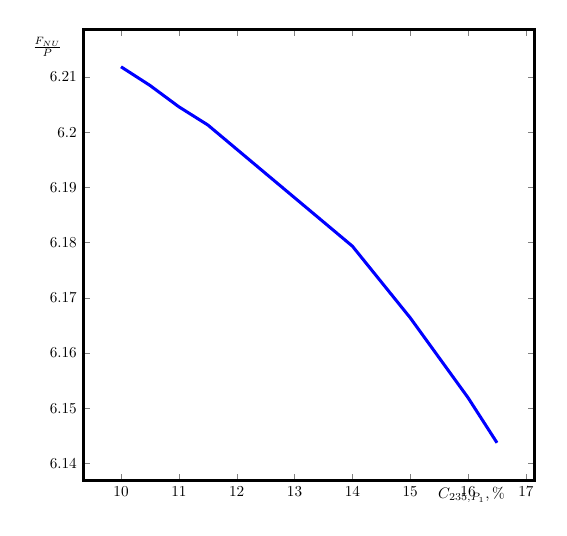
\begin{tikzpicture}[,
scale=0.55]
\begin{axis}[
  xlabel style = {{at={(axis description cs:.86,0)}}},
  ylabel = {$\frac{F_{NU}}{P}$},
  ylabel style = {{at={(axis description cs:-0.08,.925)},rotate=270,anchor=south}},
  xlabel = {$C_{235,P_1}, \%$},
  width=12cm, height=12cm, line width=2pt
]

\addplot+[mark=none,
  mark = {none}
] coordinates {
  (10.0, 6.211837137895875)
  (10.5, 6.208465161178772)
  (11.0, 6.204591108947001)
  (11.5, 6.201302679518179)
  (12.5, 6.192513286744336)
  (14.000000000000002, 6.1793427012521605)
  (15.0, 6.166360179618584)
  (16.0, 6.1518823803571845)
  (16.5, 6.143728605907763)
};

\end{axis}
\end{tikzpicture}


\caption{{Зависимость расхода природного урана от концентрации $^{235}$U в потоке легкой фракции первого каскада ($P_1$){\label{pFoP1tr}}}}
    \end{minipage}
\end{figure}

\begin{figure}[ht]
    \centering
    \begin{minipage}{.5\textwidth}
        \centering
        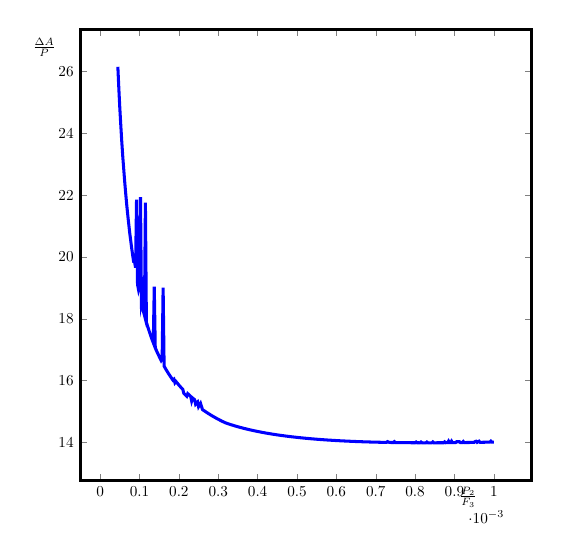
\begin{tikzpicture}[,
scale=0.55]
\begin{axis}[
  xlabel style = {{at={(axis description cs:.86,0)}}},
  ylabel = {$\frac{\Delta A}{P}$},
  ylabel style = {{at={(axis description cs:-0.08,.925)},rotate=270,anchor=south}},
  xlabel = {$\frac{P_2}{F_3}$},
  width=12cm, height=12cm, line width=2pt
]

\addplot+[
  mark = {none}
] coordinates {
  (4.5e-5, 26.15180324127409)
  (4.75e-5, 25.451483673850934)
  (5.0e-5, 24.81355435407544)
  (5.25e-5, 24.256668896511552)
  (5.5e-5, 23.721400602529187)
  (5.75e-5, 23.244994988366884)
  (6.25e-5, 22.417516089355775)
  (6.5e-5, 22.045451962222476)
  (6.75e-5, 21.694758695157482)
  (7.0e-5, 21.37641716088019)
  (7.25e-5, 21.08004269098302)
  (7.5e-5, 20.792444385988087)
  (7.75e-5, 20.54464200082422)
  (8.0e-5, 20.29575265646562)
  (8.25e-5, 20.067256591254463)
  (8.5e-5, 19.852207822335032)
  (8.75e-5, 19.84003824334713)
  (9.0e-5, 19.649959454559376)
  (9.25e-5, 21.852310152697022)
  (9.5e-5, 19.108596199465666)
  (9.75e-5, 18.94238278064752)
  (0.0001, 19.070401499547984)
  (0.0001025, 21.935876107087857)
  (0.000105, 18.497803839593637)
  (0.0001075, 18.652076695333296)
  (0.00011, 18.23920919755742)
  (0.0001125, 18.114995663203505)
  (0.000115, 21.754019050220766)
  (0.0001175, 17.886884181655226)
  (0.00012, 17.77890608735422)
  (0.0001225, 17.67934861763396)
  (0.000125, 17.58078713665917)
  (0.0001275, 17.486081848332706)
  (0.00013, 17.3921722726124)
  (0.0001325, 17.305605866088317)
  (0.000135, 17.22295946267274)
  (0.0001375, 19.039137093294432)
  (0.00014, 17.069125711027862)
  (0.0001425, 16.98588560623809)
  (0.000145, 16.91282293893103)
  (0.0001475, 16.849790370930215)
  (0.00015, 16.775432197699146)
  (0.0001525, 16.707955014972097)
  (0.000155, 16.64544023485686)
  (0.0001575, 16.695884642390343)
  (0.00016, 19.004187207843206)
  (0.0001625, 16.464092120988994)
  (0.000165, 16.40899813466505)
  (0.0001675, 16.35254739679298)
  (0.00017, 16.301162745710943)
  (0.0001725, 16.248390380176055)
  (0.000175, 16.1994596180242)
  (0.00018, 16.103377600300988)
  (0.0001825, 16.056202986712076)
  (0.000185, 16.01049738220184)
  (0.0001875, 16.038872206315393)
  (0.00019, 15.928463415087135)
  (0.0001925, 15.970206315994817)
  (0.0002, 15.853866565709696)
  (0.000205, 15.781026612126869)
  (0.0002075, 15.745919904191393)
  (0.00021, 15.711646877031962)
  (0.0002125, 15.586760004809785)
  (0.000215, 15.553571056413308)
  (0.0002175, 15.521970202579933)
  (0.00022, 15.49039446186472)
  (0.0002225, 15.57542758684126)
  (0.000225, 15.54554935867188)
  (0.0002275, 15.516294523368096)
  (0.00023, 15.487673486651337)
  (0.0002325, 15.337460360531981)
  (0.000235, 15.432376360147153)
  (0.00024, 15.379315083693406)
  (0.0002425, 15.233361981041599)
  (0.0002475, 15.303727102875856)
  (0.00025, 15.154069063717298)
  (0.000255, 15.260206634148386)
  (0.00026, 15.059669420287163)
  (0.0002625, 15.03731248885069)
  (0.000265, 15.015930878240269)
  (0.0002675, 14.994460951934064)
  (0.00027, 14.972709755415252)
  (0.0002725, 14.951968005765918)
  (0.000275, 14.932100398214217)
  (0.0002775, 14.91155593381691)
  (0.0002825, 14.872562010045831)
  (0.000285, 14.85406778510983)
  (0.0002925, 14.798039917569273)
  (0.0003, 14.746622005757935)
  (0.0003025, 14.72973293069095)
  (0.000305, 14.713158028405402)
  (0.00031, 14.680671047763166)
  (0.0003175, 14.635595223496066)
  (0.0003225, 14.612532379249187)
  (0.000325, 14.601505867379858)
  (0.0003275, 14.59094348046876)
  (0.00033, 14.580579412618821)
  (0.0003325, 14.570392158018317)
  (0.00034, 14.540964016779608)
  (0.0003425, 14.531376271769819)
  (0.0003475, 14.512947479354697)
  (0.00035, 14.503814919387265)
  (0.0003525, 14.494982802282655)
  (0.0003575, 14.47769609746605)
  (0.00036, 14.469262787504848)
  (0.000365, 14.452824241642517)
  (0.0003675, 14.444816108213743)
  (0.00037, 14.436927571313214)
  (0.000375, 14.421606190322995)
  (0.0003775, 14.41404865552997)
  (0.00038, 14.406669770129067)
  (0.0003825, 14.399409359069347)
  (0.0003875, 14.385239351943039)
  (0.00039, 14.378324909289926)
  (0.0003925, 14.371565343349861)
  (0.000395, 14.36481879581666)
  (0.0003975, 14.358237101736671)
  (0.0004025, 14.345371769979858)
  (0.000405, 14.339283684507736)
  (0.0004075, 14.332927322839454)
  (0.00041, 14.326822562168047)
  (0.0004125, 14.320836527915363)
  (0.000415, 14.314966199734164)
  (0.0004175, 14.309138266915069)
  (0.00042, 14.30345315454885)
  (0.0004225, 14.297856613223416)
  (0.0004275, 14.286814605950642)
  (0.00043, 14.282657355836237)
  (0.0004325, 14.276227184245947)
  (0.00044, 14.26079729513473)
  (0.0004425, 14.255847134073255)
  (0.0004475, 14.24612676044339)
  (0.00045, 14.241385542247482)
  (0.0004525, 14.23685307006)
  (0.000455, 14.232119099379661)
  (0.0004575, 14.22790240138011)
  (0.00046, 14.223127759679366)
  (0.0004625, 14.218751874550591)
  (0.0004675, 14.210154571057982)
  (0.00047, 14.205967225901595)
  (0.000475, 14.197770516122743)
  (0.0004775, 14.1939187333443)
  (0.0004825, 14.185936176939526)
  (0.0004875, 14.17833578668856)
  (0.00049, 14.174775484060522)
  (0.0004925, 14.17097799834162)
  (0.000495, 14.16751167886886)
  (0.0004975, 14.163828159467268)
  (0.0005, 14.160345364970757)
  (0.000505, 14.153514590730822)
  (0.0005125, 14.14366782203476)
  (0.000515, 14.140484919461683)
  (0.0005175, 14.137390689003247)
  (0.00052, 14.134263207850823)
  (0.0005225, 14.131225071657102)
  (0.000525, 14.12824157687673)
  (0.0005275, 14.125326855716988)
  (0.00053, 14.12238849231356)
  (0.0005325, 14.119528671477084)
  (0.000535, 14.116764351968255)
  (0.0005375, 14.113947704402081)
  (0.0005425, 14.10856175829401)
  (0.0005475, 14.103309813695992)
  (0.00055, 14.100746466474202)
  (0.0005525, 14.098226901086964)
  (0.000555, 14.095745613847495)
  (0.0005625, 14.088529073959668)
  (0.000565, 14.086212849039716)
  (0.0005675, 14.083912508292048)
  (0.0005725, 14.0794536355518)
  (0.000575, 14.077272667585651)
  (0.0005775, 14.07511564985152)
  (0.00058, 14.073016063600924)
  (0.0005825, 14.070939198496818)
  (0.0005925, 14.062957496899262)
  (0.000595, 14.06104517181989)
  (0.0005975, 14.059165844106115)
  (0.0006, 14.057318344342345)
  (0.000605, 14.053728895265463)
  (0.0006075, 14.051962329443565)
  (0.00061, 14.050235967126095)
  (0.0006175, 14.045236613254088)
  (0.00062, 14.043670961115694)
  (0.0006225, 14.042060679960777)
  (0.000625, 14.040495657069696)
  (0.0006275, 14.038975105589358)
  (0.0006325, 14.036017342330886)
  (0.000635, 14.034573764094564)
  (0.0006375, 14.033246657142143)
  (0.00064, 14.031759099401546)
  (0.0006425, 14.030392786031463)
  (0.000645, 14.029062861747503)
  (0.0006475, 14.027756978171723)
  (0.00065, 14.026445577139667)
  (0.000655, 14.023950284157925)
  (0.00066, 14.021548636717458)
  (0.0006625, 14.020365794076392)
  (0.0006675, 14.018099610968063)
  (0.0006725, 14.015925108585357)
  (0.000675, 14.014886573806585)
  (0.0006775, 14.013852212000463)
  (0.00068, 14.012845947098914)
  (0.000685, 14.010914163650904)
  (0.0006875, 14.00996900661053)
  (0.00069, 14.009015337072713)
  (0.0006925, 14.008120684083831)
  (0.000695, 14.007238985093773)
  (0.0006975, 14.00636167329846)
  (0.0007025, 14.004716489588432)
  (0.000705, 14.003896588109722)
  (0.0007075, 14.003130407776826)
  (0.00071, 14.002351586895864)
  (0.0007125, 14.001776886278833)
  (0.000715, 14.000899744690571)
  (0.0007175, 14.000177755050164)
  (0.00072, 13.99950717007519)
  (0.0007225, 13.998822054348429)
  (0.000725, 13.998396927947178)
  (0.0007275, 13.997556432809128)
  (0.00073, 14.023329679211498)
  (0.000735, 13.995750299201987)
  (0.0007375, 13.995426618805816)
  (0.00074, 13.994661820807627)
  (0.0007425, 13.994117746852606)
  (0.000745, 13.993623911343047)
  (0.0007475, 14.022230528893108)
  (0.00075, 13.992637864545845)
  (0.0007525, 13.992194892994346)
  (0.000755, 13.991749124735525)
  (0.0007575, 13.991323430704128)
  (0.00076, 13.990894140752003)
  (0.0007625, 13.990498541966543)
  (0.000765, 13.990136010707063)
  (0.0007675, 13.989779483332779)
  (0.00077, 13.989747089334257)
  (0.0007725, 13.989132693170419)
  (0.000775, 13.988806458428524)
  (0.0007775, 13.988466922689748)
  (0.00078, 13.988217962397295)
  (0.0007825, 13.987993865974076)
  (0.000785, 13.987626958427715)
  (0.00079, 13.987170181880238)
  (0.0007925, 13.986937951780126)
  (0.000795, 13.986752175164773)
  (0.0008, 13.98639036325982)
  (0.0008025, 14.010015998336572)
  (0.000805, 13.98606488610128)
  (0.0008075, 13.985947992317387)
  (0.00081, 13.985831146518796)
  (0.0008125, 13.985725100385531)
  (0.000815, 14.010664730315042)
  (0.0008175, 13.98553512414024)
  (0.00082, 13.98548452418285)
  (0.0008225, 13.985423626642577)
  (0.000825, 13.98536854757829)
  (0.0008275, 13.985360010245367)
  (0.00083, 14.009689675223116)
  (0.0008325, 13.985949138939377)
  (0.000835, 13.985632280086502)
  (0.0008375, 13.98536195269173)
  (0.00084, 13.985580693651148)
  (0.0008425, 13.985426598544604)
  (0.000845, 14.013343786715897)
  (0.0008475, 13.98557229188252)
  (0.00085, 13.985640421938777)
  (0.0008525, 13.985744582486383)
  (0.000855, 13.985849029972613)
  (0.0008575, 13.98598412993115)
  (0.00086, 13.986181980225746)
  (0.0008625, 13.98639774033376)
  (0.000865, 13.986363941442209)
  (0.0008675, 13.986536233871712)
  (0.00087, 13.98671143883155)
  (0.0008725, 13.986886479038683)
  (0.000875, 14.015511512190486)
  (0.0008775, 13.987269922587153)
  (0.00088, 13.98769897913355)
  (0.0008825, 13.987728902939049)
  (0.000885, 14.040200158536644)
  (0.0008875, 13.988210303018073)
  (0.00089, 13.98846148485972)
  (0.0008925, 14.038913750502719)
  (0.000895, 13.988998258039988)
  (0.0008975, 13.98930459229019)
  (0.0009, 13.98957132311646)
  (0.0009025, 13.990045129555016)
  (0.000905, 14.01833197751597)
  (0.0009075, 14.018721714444826)
  (0.0009125, 14.019426540236207)
  (0.000915, 13.991581407608297)
  (0.0009175, 13.991931358679736)
  (0.00092, 13.992306286612768)
  (0.0009225, 14.026591606270818)
  (0.000925, 13.993257295209357)
  (0.0009275, 13.993486468898679)
  (0.00093, 13.993923780174368)
  (0.0009325, 13.994346284392027)
  (0.000935, 13.99475071959476)
  (0.0009375, 13.99520500750999)
  (0.00094, 13.995639609457296)
  (0.0009425, 13.996151792457278)
  (0.000945, 13.996564161385766)
  (0.0009475, 13.997283075781324)
  (0.00095, 13.997579947818059)
  (0.0009525, 14.02690626696025)
  (0.000955, 14.035459521510361)
  (0.0009575, 13.999055564765778)
  (0.0009625, 14.036709824425419)
  (0.000965, 14.000640000331282)
  (0.0009675, 14.001174054257769)
  (0.00097, 14.001710147697299)
  (0.0009725, 14.002286971994332)
  (0.000975, 14.002830011955089)
  (0.0009775, 14.00364737872194)
  (0.00098, 14.00424409804577)
  (0.0009825, 14.00459199112613)
  (0.000985, 14.00540872395666)
  (0.00099, 14.006428896043909)
  (0.0009925, 14.039032191498098)
  (0.000995, 14.00781033724011)
  (0.0009975, 14.008449002142314)
  (0.001, 14.008960663325713)
};

\end{axis}
\end{tikzpicture}


  \caption{{Зависимость удельного расхода работы разделения от доли $P_2$ в питании третьего каскада $F_3${\label{FnuP1tr2}}}}
  \end{minipage}%
    \begin{minipage}{.5\textwidth}
      \centering
      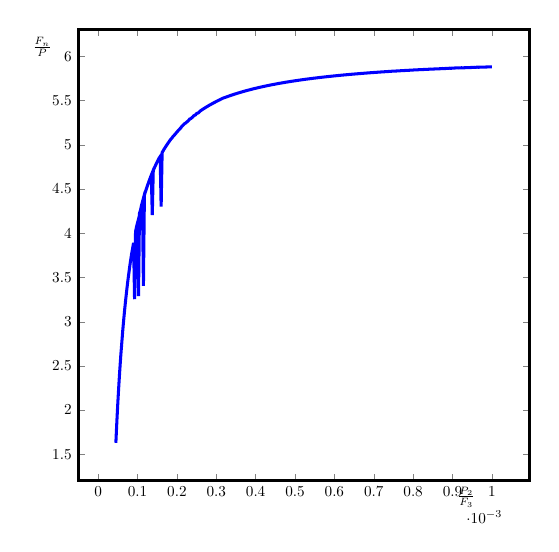
\begin{tikzpicture}[,
scale=0.55]
\begin{axis}[
  xlabel style = {{at={(axis description cs:.86,0)}}},
  ylabel = {$\frac{F_n}{P}$},
  ylabel style = {{at={(axis description cs:-0.08,.925)},rotate=270,anchor=south}},
  xlabel = {$\frac{P_2}{F_3}$},
  width=12cm, height=12cm, line width=2pt
]

\addplot+[
  mark = {none}
] coordinates {
  (4.5e-5, 1.630156602642588)
  (4.75e-5, 1.8686035233107865)
  (5.0e-5, 2.0840739633443652)
  (5.25e-5, 2.2770980190175534)
  (5.5e-5, 2.4551079867071217)
  (5.75e-5, 2.616612742979595)
  (6.25e-5, 2.899820770046827)
  (6.5e-5, 3.0256276124464088)
  (6.75e-5, 3.142709999606133)
  (7.0e-5, 3.2507461038251266)
  (7.25e-5, 3.351330044564392)
  (7.5e-5, 3.447256567547202)
  (7.75e-5, 3.5330314920229875)
  (8.0e-5, 3.6160923510574365)
  (8.25e-5, 3.693500545366085)
  (8.5e-5, 3.7663525607280195)
  (8.75e-5, 3.8272108671245606)
  (9.0e-5, 3.892031989353772)
  (9.25e-5, 3.253857367296101)
  (9.5e-5, 4.018958181546876)
  (9.75e-5, 4.074545626716676)
  (0.0001, 4.117145748719276)
  (0.0001025, 3.2881703068936634)
  (0.000105, 4.224685556736612)
  (0.0001075, 4.259652283393855)
  (0.00011, 4.312670561823864)
  (0.0001125, 4.354334309147699)
  (0.000115, 3.405092803802421)
  (0.0001175, 4.431573734692637)
  (0.00012, 4.467997786920639)
  (0.0001225, 4.502188801858757)
  (0.000125, 4.535543490345522)
  (0.0001275, 4.567590072608803)
  (0.00013, 4.5988795574826815)
  (0.0001325, 4.628323577214412)
  (0.000135, 4.656608190287754)
  (0.0001375, 4.204675662378239)
  (0.00014, 4.710001217968937)
  (0.0001425, 4.736484499318977)
  (0.000145, 4.761194415557112)
  (0.0001475, 4.784205231655417)
  (0.00015, 4.807940081061378)
  (0.0001525, 4.830464881282693)
  (0.000155, 4.851875881293119)
  (0.0001575, 4.867481406490402)
  (0.00016, 4.300589000390198)
  (0.0001625, 4.912883582128574)
  (0.000165, 4.931760657445961)
  (0.0001675, 4.950473009460712)
  (0.00017, 4.9681795591866225)
  (0.0001725, 4.98574869081551)
  (0.000175, 5.002517986107485)
  (0.00018, 5.034949347336077)
  (0.0001825, 5.050633132760592)
  (0.000185, 5.065878935391997)
  (0.0001875, 5.076633231220666)
  (0.00019, 5.0942694919641935)
  (0.0001925, 5.1044514709183035)
  (0.0002, 5.14425035643007)
  (0.000205, 5.169166968348352)
  (0.0002075, 5.18117552169505)
  (0.00021, 5.192898516007673)
  (0.0002125, 5.208761261725701)
  (0.000215, 5.219940009181771)
  (0.0002175, 5.230765472201858)
  (0.00022, 5.241425624261419)
  (0.0002225, 5.2468741768133285)
  (0.000225, 5.257083666900405)
  (0.0002275, 5.267069952427781)
  (0.00023, 5.276839447849837)
  (0.0002325, 5.291984961020257)
  (0.000235, 5.295752306531202)
  (0.00024, 5.313879941356744)
  (0.0002425, 5.327697887664804)
  (0.0002475, 5.339700159928005)
  (0.00025, 5.353528318567743)
  (0.000255, 5.363294483070997)
  (0.00026, 5.385092360758454)
  (0.0002625, 5.3925802565671175)
  (0.000265, 5.399815850519798)
  (0.0002675, 5.407014255363641)
  (0.00027, 5.414209005034644)
  (0.0002725, 5.421153215991465)
  (0.000275, 5.427871725567347)
  (0.0002775, 5.43467052323668)
  (0.0002825, 5.447708063628412)
  (0.000285, 5.453960976060155)
  (0.0002925, 5.472549480377606)
  (0.0003, 5.48983766779579)
  (0.0003025, 5.4954716603304465)
  (0.000305, 5.50100645414024)
  (0.00031, 5.5118291899412855)
  (0.0003175, 5.528856334174999)
  (0.0003225, 5.5362652438929185)
  (0.000325, 5.540126317712696)
  (0.0003275, 5.544192996598803)
  (0.00033, 5.548194125682606)
  (0.0003325, 5.552133402673498)
  (0.00034, 5.563767522463729)
  (0.0003425, 5.567309391451358)
  (0.0003475, 5.574722569760859)
  (0.00035, 5.5781978395156635)
  (0.0003525, 5.5816034898750395)
  (0.0003575, 5.5885218054362875)
  (0.00036, 5.591791104313636)
  (0.000365, 5.598345725493597)
  (0.0003675, 5.6016249488933)
  (0.00037, 5.604718148610841)
  (0.000375, 5.61104506807085)
  (0.0003775, 5.613941003649226)
  (0.00038, 5.616935974751245)
  (0.0003825, 5.619887248927881)
  (0.0003875, 5.625675358680409)
  (0.00039, 5.628512522529417)
  (0.0003925, 5.631438786094255)
  (0.000395, 5.634331018009551)
  (0.0003975, 5.636801468744348)
  (0.0004025, 5.642150161798115)
  (0.000405, 5.644987536199008)
  (0.0004075, 5.647507829466967)
  (0.00041, 5.649984986134032)
  (0.0004125, 5.652445275418484)
  (0.000415, 5.655081914385988)
  (0.0004175, 5.657402930653026)
  (0.00042, 5.659944229228747)
  (0.0004225, 5.662468082076186)
  (0.0004275, 5.666952746932445)
  (0.00043, 5.669730210383194)
  (0.0004325, 5.671696276073403)
  (0.00044, 5.678258000123561)
  (0.0004425, 5.68053626151911)
  (0.0004475, 5.684725938465346)
  (0.00045, 5.686831382860853)
  (0.0004525, 5.689096089853846)
  (0.000455, 5.690971165867154)
  (0.0004575, 5.693282182985295)
  (0.00046, 5.6950739768339345)
  (0.0004625, 5.697092361755652)
  (0.0004675, 5.7009704422309095)
  (0.00047, 5.702836782944285)
  (0.000475, 5.706617841575625)
  (0.0004775, 5.708676741708998)
  (0.0004825, 5.712135106481107)
  (0.0004875, 5.715767293356317)
  (0.00049, 5.7176584665032415)
  (0.0004925, 5.719289458862801)
  (0.000495, 5.721127489810162)
  (0.0004975, 5.722696937069765)
  (0.0005, 5.7243330897349125)
  (0.000505, 5.727686378837759)
  (0.0005125, 5.732531858729144)
  (0.000515, 5.734141514834877)
  (0.0005175, 5.735778225624764)
  (0.00052, 5.737244853459936)
  (0.0005225, 5.738798143730568)
  (0.000525, 5.740270387381419)
  (0.0005275, 5.741891722964919)
  (0.00053, 5.743330800917759)
  (0.0005325, 5.744790569862921)
  (0.000535, 5.7463248462625325)
  (0.0005375, 5.747698529837878)
  (0.0005425, 5.7504807598222705)
  (0.0005475, 5.753378400713989)
  (0.00055, 5.754673469325145)
  (0.0005525, 5.756037362453978)
  (0.000555, 5.757389302900871)
  (0.0005625, 5.761409887790838)
  (0.000565, 5.7626631949611795)
  (0.0005675, 5.763995355881044)
  (0.0005725, 5.766489764960659)
  (0.000575, 5.767741329191286)
  (0.0005775, 5.7690258627805076)
  (0.00058, 5.770209556253116)
  (0.0005825, 5.771427026188225)
  (0.0005925, 5.776210566901978)
  (0.000595, 5.77738928485018)
  (0.0005975, 5.778541693104508)
  (0.0006, 5.779682209610915)
  (0.000605, 5.78189185571987)
  (0.0006075, 5.783029481932145)
  (0.00061, 5.784130503417717)
  (0.0006175, 5.787390354490052)
  (0.00062, 5.788525695271179)
  (0.0006225, 5.789466009482686)
  (0.000625, 5.790550176774105)
  (0.0006275, 5.791563469385086)
  (0.0006325, 5.793588239219532)
  (0.000635, 5.794597024399381)
  (0.0006375, 5.795749086011606)
  (0.00064, 5.796601012777678)
  (0.0006425, 5.797635975947155)
  (0.000645, 5.798544085392858)
  (0.0006475, 5.799627600450835)
  (0.00065, 5.800506239934855)
  (0.000655, 5.802368489607907)
  (0.00066, 5.804219428523848)
  (0.0006625, 5.805175478715322)
  (0.0006675, 5.806988954918959)
  (0.0006725, 5.808773258693746)
  (0.000675, 5.809616809396662)
  (0.0006775, 5.810605560695505)
  (0.00068, 5.811357273661609)
  (0.000685, 5.813177580655779)
  (0.0006875, 5.81402286657737)
  (0.00069, 5.814843858063425)
  (0.0006925, 5.815585982750028)
  (0.000695, 5.816410667123485)
  (0.0006975, 5.817264844315089)
  (0.0007025, 5.818936365529603)
  (0.000705, 5.819681209709617)
  (0.0007075, 5.820438564405873)
  (0.00071, 5.821260251426856)
  (0.0007125, 5.822201846532028)
  (0.000715, 5.822779482497837)
  (0.0007175, 5.823582723331287)
  (0.00072, 5.824309530800732)
  (0.0007225, 5.82510126507946)
  (0.000725, 5.826017303426601)
  (0.0007275, 5.826560008125806)
  (0.00073, 5.828764133386643)
  (0.000735, 5.828792402043945)
  (0.0007375, 5.829685272038274)
  (0.00074, 5.830195868624448)
  (0.0007425, 5.830940988741253)
  (0.000745, 5.831612822918468)
  (0.0007475, 5.833811991332199)
  (0.00075, 5.833038210787387)
  (0.0007525, 5.833694213704382)
  (0.000755, 5.83446729199153)
  (0.0007575, 5.8350565591065555)
  (0.00076, 5.835762899283395)
  (0.0007625, 5.836430875798403)
  (0.000765, 5.837061725808435)
  (0.0007675, 5.8378193886450775)
  (0.00077, 5.838608409480933)
  (0.0007725, 5.83915042593583)
  (0.000775, 5.839632753984306)
  (0.0007775, 5.840302605710987)
  (0.00078, 5.840902630716486)
  (0.0007825, 5.841723095217284)
  (0.000785, 5.842223005731545)
  (0.00079, 5.843426771708657)
  (0.0007925, 5.844070187847865)
  (0.000795, 5.844738500875216)
  (0.0008, 5.845844043542308)
  (0.0008025, 5.8477958092457865)
  (0.000805, 5.847057126533179)
  (0.0008075, 5.847703590324903)
  (0.00081, 5.848191140419607)
  (0.0008125, 5.848767069718393)
  (0.000815, 5.850716347088039)
  (0.0008175, 5.849939455589227)
  (0.00082, 5.850471255786386)
  (0.0008225, 5.8510388924719905)
  (0.000825, 5.851655712279825)
  (0.0008275, 5.852138618304741)
  (0.00083, 5.854039928474564)
  (0.0008325, 5.853545419026327)
  (0.000835, 5.853994796859881)
  (0.0008375, 5.854398014452639)
  (0.00084, 5.855030864096904)
  (0.0008425, 5.85539845061953)
  (0.000845, 5.857301033304584)
  (0.0008475, 5.85641406976861)
  (0.00085, 5.856933992725324)
  (0.0008525, 5.857445614261717)
  (0.000855, 5.857955246047224)
  (0.0008575, 5.858580708637048)
  (0.00086, 5.858905939382217)
  (0.0008625, 5.859653208073091)
  (0.000865, 5.859963519073614)
  (0.0008675, 5.860455081474957)
  (0.00087, 5.860940322450788)
  (0.0008725, 5.861433474760401)
  (0.000875, 5.863307857393135)
  (0.0008775, 5.862468339542952)
  (0.00088, 5.86306315397651)
  (0.0008825, 5.863337006784049)
  (0.000885, 5.8654634918405115)
  (0.0008875, 5.864272793182839)
  (0.00089, 5.864741024005697)
  (0.0008925, 5.866829579039055)
  (0.000895, 5.865651906526707)
  (0.0008975, 5.866214326281121)
  (0.0009, 5.866588675704485)
  (0.0009025, 5.867181536266297)
  (0.000905, 5.868817728997574)
  (0.0009075, 5.869258341849851)
  (0.0009125, 5.870128149558689)
  (0.000915, 5.869197509979065)
  (0.0009175, 5.8697047791363754)
  (0.00092, 5.870074456565848)
  (0.0009225, 5.871915144168207)
  (0.000925, 5.870811195709174)
  (0.0009275, 5.871339473661354)
  (0.00093, 5.87172306143217)
  (0.0009325, 5.872134344796738)
  (0.000935, 5.872577996675054)
  (0.0009375, 5.872962427431372)
  (0.00094, 5.873388050735082)
  (0.0009425, 5.873883739671422)
  (0.000945, 5.874234997281066)
  (0.0009475, 5.874754220119411)
  (0.00095, 5.875071957258566)
  (0.0009525, 5.876685602372115)
  (0.000955, 5.877178652875113)
  (0.0009575, 5.8761054965418635)
  (0.0009625, 5.878317464695467)
  (0.000965, 5.8772431589796525)
  (0.0009675, 5.8776268515615975)
  (0.00097, 5.878018028221509)
  (0.0009725, 5.8783690289954125)
  (0.000975, 5.878811173827366)
  (0.0009775, 5.878999842811271)
  (0.00098, 5.879665067745371)
  (0.0009825, 5.879845284292096)
  (0.000985, 5.880087007393254)
  (0.00099, 5.880897927375689)
  (0.0009925, 5.8826081867337665)
  (0.000995, 5.881756187473633)
  (0.0009975, 5.882102171740465)
  (0.001, 5.882301659117415)
};

\end{axis}
\end{tikzpicture}


\caption{{Зависимость расхода природного урана от доли $P_2$ в питании третьего каскада $F_3${\label{pFoP1tr2}}}}
    \end{minipage}
\end{figure}

\section{Оценка эффективности тройного каскада по различным критериям}\label{MDKefficiency}

Из анализа результатов оценки эффективности модифицированного двойного каскада по различным критериям, приведенных в разделе \ref{MDKefficiency}, можно заключить, что получаемый в легкой фракции поток $P_2$ целесообразно вовлекать только в случаях, когда на обогащение $^{235}$U в $P_2$ введено ограничение 20\%, так как в этом случае $P_2$ на порядки меньше загрязнен изотопом $^{232}$U, а самого побочного продукта получается на порядки больше.

Исходя из этого, в данном разделе приведены результаты оценки эффективности схемы тройного каскада: результирующие параметры предложенной каскадной схемы при ее оптимизации по различным критериям эффективности (\ref{DeltaA})-(\ref{RecR2}). Рассмотренные примеры отвечают приведенной в разделе \ref{statement} постановке задачи. Расчёты проведены на примере двух изотопных составов регенерата (табл. \ref{is_compositions_2_5}), характеризующихся различным исходным содержанием четных изотопов и $^{235}$U. Внешние условия приняты теми же, что и в рассмотренном выше примере. 

Основные параметры каскадной схемы, оптимизированной по одному из критериев эффективности представлены в таблице \ref{2opt1_int}.
Набор оптимальных параметров каскадной схемы для каждого из критериев соответствует отдельной колонке в указанных таблицах. 
Массы производимого на концах каскадов материала расчитаны исходя из необходимости прозвести 1 т металлического урана конечного НОУ-продукта, что соответствует 1479 кг гексафторида урана $UF_6$ (за счет присутствия фтора в рабочей смеси обогащаемого урана).

\begin{table}
    \begin{tabular}{|c|c|c|c|c|}
    \Xhline{2\arrayrulewidth}
    \diagbox{П}{К} & $(Y_f)_\text{max}$ & $(Y_{E})_\text{max}$ & $(\delta(\frac{\Delta A}{P}))_\text{min}$ & $(\delta(\frac{F_{NU}}{P}))_\text{min}$ \\ \hline
    $Y_f, \%$ & $72.61$ & 7,393 & 7,393 & $1.584$\\ \hline
    $Y_{E}, \%$ & $77.85$ & $87,27$ & 87,27 & $64.0$\\ \hline
    $\delta(\frac{\Delta A}{P}), \%$ & $-6.937$ & 1,36 & 1,36 & $-40.03$\\ \hline
    $\delta(\frac{F_{NU}}{P}), \%$ & $22.11$ & 21,41 & 21,41 & $35.33$\\ \hline
    $C_{232,P}, \%$ & $5.0e-7$ & $5.0e-7$ & $5.0e-7$ & $3.793e-7$\\ \hline
    $C_{235,P}, \%$ & $5.115$ & $5.146$ & $5.146$ & $5.086$\\ \hline
    $C_{236,P}, \%$ & $0.5691$ & $0.6775$ & $0.6775$ & $0.469$\\ \hline
    $M_{k1}$ & $238$ & $238$ & $238$ & $238$\\ \hline
    $M_{k2}$ & $234$ & $232$ & $232$ & $238$\\ \hline
    $C_{235,P_{1}}, \%$ & $11.61$ & 6,799 & 6,799 & $13.56$\\ \hline
    $C_{235,W_{2}}, \%$ & $10.62$ & 6,458 & 6,458 & $12.58$\\ \hline
    $C_{235,P_{n}}, \%$ & $4.523$ & $4.875$ & $4.875$ & $5.168$\\ \hline
    $C_{235,P_{2}}, \%$ & $18.26$ & $19.26$ & $19.26$ & $16.26$\\ \hline
    $C_{232,P_{1}}, \%$ & $5.74e-6$ & $3.34e-6$ & $4.34e-6$ & $6.71e-6$\\ \hline
    $C_{232,P_{2}}, \%$ & $1.41e-5$ & 2,366e-5 & 2,366e-5 & $9.811e-6$\\ \hline    
    $P_1$, кг  & $158.7$ & 272,6 & 272,6 & $135.7$\\ \hline
    $W_2$, кг  & $138.1$ & 265,4 & 265,4 & $99.75$\\ \hline
    $P_n$, кг  & $1263.0$ & 1181,0 & 1181,0 & $915.3$\\ \hline
    $P_2$, кг  & $20.55$ & 7,265 & 7,265 & $35.97$\\ \hline
    $P_3$, кг  & $77.58$ & 33,11 & 33,11 & $464.0$\\ \hline
    $\frac{P_{2}}{F_3}$  & $0.001365$ & $1.0e-5$ & $1.0e-5$ & $1.0e-5$\\ \hline
    $C_{235,W_{3}}, \%$ & $0.1299$ & $0.13$ & $0.13$ & $0.1298$\\ \hline
    $C_{235,P_{3}}, \%$ & $4.959$ & $4.309$ & $4.309$ & $3.312$\\ \hline
\end{tabular}
\caption{Параметры схемы тройного каскада с НОУ-разбавителем при различных критериях оптимизации для обогащения регенерата состава 1.{\label{3opt2}}}
\end{table}

% \textcolor{red}{проблема в том, что решения упираются в верхнюю границу $C_{235,W_{3}}$ и нижнюю $\frac{P_{2}}{F_3}$}


\subsection{Сравнение интегральных параметров для способов утилизации побочного продукта модифицированного двойного каскада}

В данном разделе представлены результаты сравнения вариантов для утилизации побочного продукта, образовавшегося в результате эксплуатации модификации двойного каскада. В качестве сравниваемых вариантов представлены  рассмотренные ранее схемы: 

\begin{enumerate}
    \item модифицированный двойной каскад с возвратом в цикл, рассмотренный в ч. \ref{P2ret} (далее -- сх. 1);
    \item схема независимой утилизации (далее -- сх. 2), рассмотренный в ч. \ref{indep_p2};
    \item тройной каскад с компенсацией $^{236}$U, рассмотренный в ч. \ref{triple_c} (далее -- сх. 3).
\end{enumerate}

Сам модифицированный каскад как базовый вариант далее будем обозначать как <<схему 1>>. В расчётах полагали, что каждая из схем должна была решить сформулированную в разделе \ref{example_trip} задачу при тех же внешних условиях и обогащаемом регенерате состава 1, а также имея ограничение на обогащение $^{235}$U в 20\%. Сравнение для данных схем, используемых для получения загрузки 1, 2 и их среднего арифметического (столбец ср.), проводили по интегральным характеристикам: $\frac{\Delta A}{P}$, $\frac{F_{NU}}{P}$, а также сравнивали расход регенерата на единицу продукта ($\frac{E}{P}$). Для сх. 1 и сх. 3 выбраны решения, соответствующие оптимуму работы разделения.

Постановка задачи соответствует приведенной в \ref{statement}, с некоторыми дополнительными входными условиями для отдельных схем.

В табл. \ref{3loop} представлены результаты сравнения интегральных показателей для перечисленных схем для питающих составов 1 и 2 регенерата, соответственно.


В данном разделе представлены результаты сравнения предложенной модификации двойного каскада с некоторыми типичными способами обогащения регенерата, рассмотренными ранее в литературе и патентах. В качестве сравниваемых вариантов каскадных схем рассмотрены следующие: 

\begin{table}
    \centering
    \renewcommand{\arraystretch}{1.2}
    \begin{tabular}{|r|c|c|c|c|c|c|c|c|c|}
      \hline
      \multirow{2}{*}{\diagbox{П}{сх.}} & \multicolumn{3}{c|}{1} & \multicolumn{3}{c|}{2} & \multicolumn{3}{c|}{3}\\
      \cline{2-10}
      & 1 & 2 & ср. & 1 & 2 & ср. & 1 & 2 & ср. \\
      \hline
      $\frac{E}{P}$     & 0,93 & 0,9489 & - & 0,93 & 1,0722 & - & 0,93 & 0,93 & 0,93 \\ \hline
      $\frac{F_{NU}}{P}$ & 6,2097 & 6,486 & 6.348 & 6,2097 & 6,3404 & - & 6,0436 & 6,0436 & 6,0436\\ \hline
      $\frac{\Delta A}{P}$ & 11,246 & 11,606 & 11,426 & 11,246 & 11,2036 & - & 11,649 & 11,649 & 11,649 \\ \hline
    \end{tabular}
\caption{Сравнение интегральных показателей схем утилизации загрязненного продукта для состава 1.{\label{3loop}}}
\end{table}
% 6.3404=(Fnu/P)MDK*(1-Padd/1000)+(Fnu/P)ord.*(Fleu/1000)=6.2097*(1-142.2/1000)+7.69*(131.82/1000)=6.2097*(1-142.2/1000)+7.69*(131.82/1000)
% 11.2036=(Anu/P)MDK*(1-Padd/1000)+(Fnu/P)ord.*(Fleu/1000)=6.2097*(1-142.2/1000)+7.69*(131.82/1000)=11.246*(1-142.2/1000)+11.81*(131.82/1000)
% "-", когда нет смысла усреднять $\frac{E}{P}$

Если при рассмотрении варианта независимой утилизации $P_2$, основную характеристическую величину $P_{+}$, соответствующую доле замещаемого природного урана, используемого для получения свежего НОУ требуемого качества, расчитывали как

\begin{equation} \label{P_plus} 
P_{+} = \frac{P_2 + F_D}{P_{add}}
\end{equation}
, где $P_{add}=P_2+F_D+F_{leu}$

, то при использовании добавки в виде $P_{add}$ для формирования загрузки 2 сх.2, интересующими показателями будут выступать:

\begin{equation} \label{Fnu_plus} 
\frac{F_{NU}}{P}=(\frac{F_{NU}}{P})_{\text{сх.1}}\cdot (1 - \frac{P_{add}}{1000}) + (\frac{F_{NU}}{P})_{ord.}\cdot \frac{F_{leu}}{1000}
\end{equation} 

\begin{equation} \label{AvsP_plus} 
\frac{\Delta A}{P}=(\frac{\Delta A}{P})_{\text{сх.1}}\cdot (1 - \frac{P_{add}}{1000}) + (\frac{\Delta A}{P})_{ord.}\cdot \frac{F_{leu}}{1000}
\end{equation} 

, исходя из того, что массовые значения $P_{add}$ и $F_{leu}$ были расчитаны на 1 т НОУ-продукта.



\subsection{Выводы по результатам исследования эффективности схемы тройного каскада}

Как результат, схема тройного каскада с НОУ-разбавителем и дополнительным разбавителем потока $P_2$, возвращаемого в цикл, позволяя в полноте решить поставленную задачу, не оставляет никакого нештатного отхода, требующего особых мер обращения. В конечном итоге образуется только штатный отход в виде отвалов $W_1$ и $W_3$ , процедуры обращения с которыми на разделительном производстве технологически отработаны. Если получить их смешением ($W_1$ и $W_3$) обедненный уран, он будет содержать изотопы $^{232,234}$U в количествах в десятки/сотни раз сниженных, относительно исходного регенерата. Следовательно, полученный в такой схеме обедненный уран может быть переведен в двуокись урана, например, при помощи установки «W-ЭХЗ». Отсутствие нештатных отходов, загрязненных четными изотопами и является отличительным достоинством рассмотренной схемы, тогда как недостатком выступают дополнительные потери работы разделения, возникающие при перемешивании потока $P_2$ и подмешиваемого к нему в качестве разбавителя ОГФУ.


В качестве итогового списка характеристических особенностей схемы тройного каскада следует обозначить следующие:

\begin{enumerate}
    \item применима для обогащения регенерированного урана в условиях многократного рецикла и позволяет получать продукт, отвечающий всем требованиям по концентрациям четных изотопов для регенерата различного исходного состава как показано на рассматриваемых входных изотопных составах;
    \item достоинством схемы является полное отсутствие нештатных отходов, требующих специального обращения, поскольку на выходе из схемы, помимо основного продукта, возникают только потоки обедненного урана в виде отвалов каскадов схемы. Причем, в отличие от схемы двойного каскада с НОУ-разбавителем, отход отсутствует при любом варианте использования: как для однократного обогащения регенерированного урана, так и в условиях постоянных поступлений партий регенерированного урана последовательных перегрузок реактора;
    \item как и предшествующие схемы, схема позволяет задействовать для воспроизводства ядерного топлива накопленный в значительных количествах обедненный уран;
    \item в схеме отделены участки обогащения регенерированного урана и участок обогащения обедненного или природного урана (каскад, расположенный на схеме слева (рис. 
    \ref{p2_withDepU})), не загрязненного четными изотопами. В дальнейшем это позволит использовать оборудование этого каскада для обогащения природного урана или другого сырьевого материала, не загрязненного четными изотопами;
    % \item получаемый в схеме отвал регенерированного урана в потока $W_1$ и $W_3$ имеет содержание изотопа $^{232}$U ниже, чем исходный регенерат. Подобный материал можно длительно хранить или отправить на переработку в установке дефторирования. В случае же необходимости дополнительного понижения концентраций четных изотопов данный поток может быть дополнительно разбавлен конечными отвалами с обогащением ниже 0,13\%. 
    \item недостатком схемы являются потери работы разделения из-за необходимости:
    \begin{enumerate}
        \item обеднять отбор первого каскада в последующем втором каскаде;
        \item смешивание потоков $W_2$ с НОУ-разбавителем $P_0$, а затем и с $P_3$ в которых различается содержание изотопа $^{235}$U;
        \item смешивания потоков $P_2$ и $F_D$ на входе в третий каскад.
    \end{enumerate}
\end{enumerate}


Слабое изменение параметров каскадной схемы в условиях многократного рецикла позволяет говорить о возможности «настройки» данной каскадной схемы на возможность работы с регенератом различных рециклов при минимальных изменениях параметров. В частности, для данной схемы возможно подобрать «унифицированный» разбавитель с фиксированным содержанием $^{235}$U, что могло бы позволить не привязывать напрямую мощности по получению разбавителя из обедненного урана (каскад III) к каскадам, работающим с регенератом. Иными словами, в этом случае разбавитель мог бы нарабатываться независимо от поступлений конкретных партий регенерата.


В качестве выводов, относящихся ко всем рассмотренным схемам, приведем следующие:
\begin{enumerate}
    \item схемы на основе двойного каскада, использующие НОУ-разбавитель, принципиально пригодны для решения задачи обогащения регенерированного урана в рамках многократного рецикла урановой составляющей топлива легководных реакторов. При этом каждая из схем имеет собственные достоинства и недостатки;
    \item характерным недостатком схемы, не предполагающей утилизацию нештатного отхода, образующегося в потоке $P_2$, является проблема с обращением с этим материалом, с высоким содержанием как четных изотопов (на 1-2 порядка выше, чем пределы для товарного НОУ) и $^{235}$U (до 20\% или, в некоторых случаях, до 90\%, в зависимости от выбранного режима работы каскадной схемы). Одним из вариантов обращения с ним, помимо схемы независимой утилизации побочного продукта легкой фракции второго каскада схемы двойного каскада с НОУ-разбавителем (рис. \ref{P2utilization}), может стать его перемешивание с отвалом первого каскада при обогащении регенерата. Оценки показали, что в этом случае возможно получить обедненный уран с приемлемым содержанием $^{232}$U (не выше $5\cdot10^{-7}$\%);
    \item характерными недостатком схемы двойного каскада с НОУ-разбавителем с возвратом потока $P_2$ в цикл (рис. \ref{P2utilizationRing}) является возврат значительной части четных изотопов на вход каскадной схемы;
    \item характерным недостатком схемы тройного каскада (рис. \ref{p2_withDepU}) являются дополнительные затраты работы разделения по отношению к схемам двойного каскада с НОУ-разбавителем, возникающие при обогащении разбавленного обедненным ураном отхода второго каскада схемы, загрязненного четными изотопами.
  \end{enumerate}

Анализ эффективности предложенных каскадных схем с точки зрения потерь $^{235}$U показал, что перспективными вариантами для дальнейшей технико-экономической проработки являются каскадные схемы двойного каскада с НОУ-разбавителем (рис. \ref{p2left}) и тройного каскада (рис. \ref{p2_withDepU}). Cхема двойного каскада с НОУ-разбавителем на каждом из рассмотренных рециклах позволяет извлечь более 80\% от массы $^{235}$U из исходного регенерированного урана, поступившего на обогащение.

Для выбора конкретного варианта каскадной схемы для организации производственного процесса, необходим детальный технико-экономический анализ каждой из схем на основе их интегральных показателей, таких как расход сырьевых материалов и работы разделения, в контексте всей цепочки ядерного топливного цикла, а также с учетом возникающих в этой цепочке изменений при использовании регенерата урана по отношению к открытому топливному циклу. Помимо этого, необходима проработка технологических проблем каждой из схем, в частности, с точки зрения возможности эксплуатации и обслуживания оборудования в условиях работы с материалами, имеющими более высокую, чем природный уран удельную активность. Например, подобные условия возникают в каскадах, концентрирующих в легкой фракции $\alpha$-активные изотопы $^{232,234}$U.

\clearpage

